%%%%%%%%%%%%%%%%%%%%%%%%%%%%%%%%%%%%%%%%%%%%%%%%%%%%%%%%%%%%%%%%%%%%%%%%%%%%%%%%
%%% Author: https://github.com/jtleek/capitalIn21stCenturyinR
%%% Author: knitr/beamer by Patrick Toche, December 2014
%%% Author: data/content by Thomas Piketty, 2013-2014
%%% This replicates a December 2014 presentation at Sao Paulo by Thomas Piketty
%%% The .Rnw file is the 'master', other files produced by knitr compilation
%%% To compile in R: library(knitr); knit("slides.Rnw");
%%% To compile in Rstudio: 'Compile PDF' menu command
%%% The 'pictures' directory contains images inserted with \includegraphics
%%% The 'figures' directory contains pdf created and inserted by knitr
%%% Delete the 'cache' directory to recreate pdf graphics
%%% The 'SaoPaulo' directory contains pdf of original powerpoint for reference
%%%%%%%%%%%%%%%%%%%%%%%%%%%%%%%%%%%%%%%%%%%%%%%%%%%%%%%%%%%%%%%%%%%%%%%%%%%%%%%%

%%% \PassOptionsToPackage loads options for packages loaded by beamer class
\PassOptionsToPackage{obeyspaces}{url}% url package loaded by hyperref
\PassOptionsToPackage{usenames,dvipsnames,svgnames}{xcolor}% named colors
\PassOptionsToPackage{%
    unicode = {false}%
    , colorlinks = {true}%
    , linkcolor = {MidnightBlue}%
    , filecolor = {MidnightBlue}%
    , citecolor = {MidnightBlue}%
    , urlcolor = {MidnightBlue}%
    , breaklinks = {false}%
    , plainpages = {true}% page number anchors as plain arabic
    , bookmarks = {true}%
    , bookmarksnumbered = {true}%
    , bookmarksopen = {true}%
    , backref = {false}%
    , pdfusetitle = {false}% false required for \includeonlyframeslist hack
    , pdfpagemode = {UseNone}% UseThumbs, UseOutlines, FullScreen, UseNone
    , pdfpagetransition = {Wipe /Di -45}%
    , pdfpagelayout = {SinglePage}%
    , pdfpagelabels = {false}% fix for beamer bug for some classes
    , pdfstartpage = {1}%
    , pdfstartview = {FitV}%
    , pdffitwindow = {false}%
    , pdfcenterwindow = {true}%
    , pdfmenubar = {true}%
    , pdfdisplaydoctitle = {true}%
}{hyperref}

%%%%%%%%%% Preamble Here %%%%%%%%%%%%%%%%%%%%%%%%%%%%%%%%%%%%%%%%%%%%%%%%%%%%%%%
\documentclass[t]{beamer}\usepackage[]{graphicx}\usepackage[]{color}
%% maxwidth is the original width if it is less than linewidth
%% otherwise use linewidth (to make sure the graphics do not exceed the margin)
\makeatletter
\def\maxwidth{ %
  \ifdim\Gin@nat@width>\linewidth
    \linewidth
  \else
    \Gin@nat@width
  \fi
}
\makeatother

\definecolor{fgcolor}{rgb}{0.345, 0.345, 0.345}
\newcommand{\hlnum}[1]{\textcolor[rgb]{0.686,0.059,0.569}{#1}}%
\newcommand{\hlstr}[1]{\textcolor[rgb]{0.192,0.494,0.8}{#1}}%
\newcommand{\hlcom}[1]{\textcolor[rgb]{0.678,0.584,0.686}{\textit{#1}}}%
\newcommand{\hlopt}[1]{\textcolor[rgb]{0,0,0}{#1}}%
\newcommand{\hlstd}[1]{\textcolor[rgb]{0.345,0.345,0.345}{#1}}%
\newcommand{\hlkwa}[1]{\textcolor[rgb]{0.161,0.373,0.58}{\textbf{#1}}}%
\newcommand{\hlkwb}[1]{\textcolor[rgb]{0.69,0.353,0.396}{#1}}%
\newcommand{\hlkwc}[1]{\textcolor[rgb]{0.333,0.667,0.333}{#1}}%
\newcommand{\hlkwd}[1]{\textcolor[rgb]{0.737,0.353,0.396}{\textbf{#1}}}%

\usepackage{framed}
\makeatletter
\newenvironment{kframe}{%
 \def\at@end@of@kframe{}%
 \ifinner\ifhmode%
  \def\at@end@of@kframe{\end{minipage}}%
  \begin{minipage}{\columnwidth}%
 \fi\fi%
 \def\FrameCommand##1{\hskip\@totalleftmargin \hskip-\fboxsep
 \colorbox{shadecolor}{##1}\hskip-\fboxsep
     % There is no \\@totalrightmargin, so:
     \hskip-\linewidth \hskip-\@totalleftmargin \hskip\columnwidth}%
 \MakeFramed {\advance\hsize-\width
   \@totalleftmargin\z@ \linewidth\hsize
   \@setminipage}}%
 {\par\unskip\endMakeFramed%
 \at@end@of@kframe}
\makeatother

\definecolor{shadecolor}{rgb}{.97, .97, .97}
\definecolor{messagecolor}{rgb}{0, 0, 0}
\definecolor{warningcolor}{rgb}{1, 0, 1}
\definecolor{errorcolor}{rgb}{1, 0, 0}
\newenvironment{knitrout}{}{} % an empty environment to be redefined in TeX

\usepackage{alltt}
%%% Select frames to be included in presentation
% \includeonlyframes{} takes a comma-separated list *without spaces*
%% spaces causes error: the % gobble up spaces
\includeonlyframes{%
TitlePage_1,%
Introduction_1,%
WTID,%
%Figure_1_1,%
Figure_8_5,%
Figure_1_2,%
ThreePoints,%
BrasilVersus,%
BrazilUSTop1,%
BrazilUSTop10,%
BrazilInequality,%
Figure_5_3,%
%Figure_5_3b,%
%Figure_5_4,%
Figure_5_5,%
Table_12_1,%
Table_12_2,%
Figure_9_8,%
Figure_14_1,%
Figure_14_2,%
Conclusions_1%
}%%%%%%%%%%%%%%%%%%%%%%%%%%%%%%%%%%%%%%%%%%%%%% list of frames for inclusion
%% !TEX root = slidesMaster.tex

% spaces causes error: the % gobble up spaces
\includeonlyframes{%
TitlePage_1%
%,Figure_1_1%
%,Figure_1_2%
,Figure_2_1%
,Figure_2_2a%
,Figure_2_2%
%,Figure_5_1%
%,Figure_5_2%
%,Figure_5_3%
%,Figure_5_3b%
%,Figure_5_4%
%,Figure_5_5%
%,Figure_5_6%
%,Figure_5_7%
%,Figure_5_8%
%,Figure_8_1%
%,Figure_8_2%
%,Figure_8_3%
%,Figure_8_4%
%,Figure_8_5%
%,Figure_8_6%
%,Figure_8_7%
%,Figure_8_8%
%,Figure_8_9%
%,Figure_8_10%
%,Figure_9_8%
%,Figure_14_1%
%,Figure_14_2%
%,WealthReturn%
%,CapitalIsBack%
%,ElasticityKL%
%,Robots%
%,WealthFuture%
%,WealthShocks%
%,InequalityUSA%
%,USAvEU%
%,MeritVNorms% 
}%% frames being debugged

%%%%%%%%%% Set Document Information %%%%%%%%%%%%%%%%%%%%%%%%%%%%%%%%%%%%%%%%%%%%
\title{Capital in the 21st Century}
\author[Thomas Piketty]{Thomas Piketty\inst{1}\inst{2}}
\institute{$^1$Paris School of Economics \\
  Sao Paulo, 26 November 2014 \bigskip\bigskip \\
  $^2$translated to beamer via knitr by Patrick Toche \\
  \href{mailto:contact@patricktoche.com}{contact@patricktoche.com} \\
  Based on collaborative effort led by Jeff Leek \\
  \url{https://github.com/jtleek/capitalIn21stCenturyinR} \\
  All copyright claims with Professor Piketty
}
\date{December 2014}

%%%%%%%%%% Set Beamer Options %%%%%%%%%%%%%%%%%%%%%%%%%%%%%%%%%%%%%%%%%%%%%%%%%%
\usetheme{piketty}

%%%%%%%%%% Load Latex Packages %%%%%%%%%%%%%%%%%%%%%%%%%%%%%%%%%%%%%%%%%%%%%%%%%
\usepackage[T1]{fontenc}% font encoding, load before inputenc
\usepackage[utf8]{inputenc}% character inputing, load after fontenc
\usepackage{lmodern}
\usepackage{booktabs}% fancy tables
\usepackage[flushleft]{threeparttable}% fancy tables
\usepackage{adjustbox}% combine with threeparttable package
\usepackage{verbatim}% pass text as unprocessed strings / comment out

%%%%%%%%%% Set Miscellani %%%%%%%%%%%%%%%%%%%%%%%%%%%%%%%%%%%%%%%%%%%%%%%%%%%%%%
\setcounter{secnumdepth}{3}%
\setcounter{tocdepth}{3}%
\setlength{\abovecaptionskip}{0pt}%
\setlength{\belowcaptionskip}{0pt}%
\renewcommand{\insertpagenumber}{}% suppress page numbers

%%%%%%%%%% Load knitr Options %%%%%%%%%%%%%%%%%%%%%%%%%%%%%%%%%%%%%%%%%%%%%%%%%%






%%%%%%%%%% Start of Document %%%%%%%%%%%%%%%%%%%%%%%%%%%%%%%%%%%%%%%%%%%%%%%%%%%
\IfFileExists{upquote.sty}{\usepackage{upquote}}{}
\begin{document}

%%%%%%%%%%%%%%%%%%%% Frame Here %%%%%%%%%%%%%%%%%%%%%%%%%%%%%%%%%%%%%%%%%%%%%%%%
\begin{frame}[label=TitlePage_1]
\maketitle% first slide with title/author information
\end{frame}
%%%%%%%%%%%%%%%%%%%% Frame Here %%%%%%%%%%%%%%%%%%%%%%%%%%%%%%%%%%%%%%%%%%%%%%%%


%%%%%%%%%%%%%%%%%%%% Frame Here %%%%%%%%%%%%%%%%%%%%%%%%%%%%%%%%%%%%%%%%%%%%%%%%
\begin{frame}[label=Introduction_1]
\frametitle{Presention layout}
\begin{itemize}
\item
This presentation is based upon Capital in the 21st century (Harvard University Press, March 2014)
\item
This book studies the global dynamics of income and wealth distribution since 18c in 20+ countries; I use historical data collected over the past 15 years with Atkinson, Saez, Postel-Vinay, Rosenthal, Alvaredo, Zucman, and 30+ others; I try to shift attention from rising income inequality to rising wealth inequality
\item
The book includes four parts:
\begin{itemize}
\item
Part 1. Income and capital
\item
Part 2. The dynamics of the capital/income ratio 
\item
Part 3. The structure of inequalities
\item
Part 4. Regulating capital in the 21st century
\end{itemize}
\item 
I will present some results from Parts 2 \& 3, focusing upon the long-run evolution of capital/income ratios and wealth concentration (\href{all graphs and series are available online}{http://piketty.pse.ens.fr/capital21c}.
\end{itemize}
\end{frame}
%%%%%%%%%%%%%%%%%%%% Frame Here %%%%%%%%%%%%%%%%%%%%%%%%%%%%%%%%%%%%%%%%%%%%%%%%


%%%%%%%%%%%%%%%%%%%% Frame Here %%%%%%%%%%%%%%%%%%%%%%%%%%%%%%%%%%%%%%%%%%%%%%%%
\begin{frame}[label=WTID]
\frametitle{The World Top Incomes Database}
\begin{figure}[t]
\begin{minipage}[b]{\textwidth}
\centering
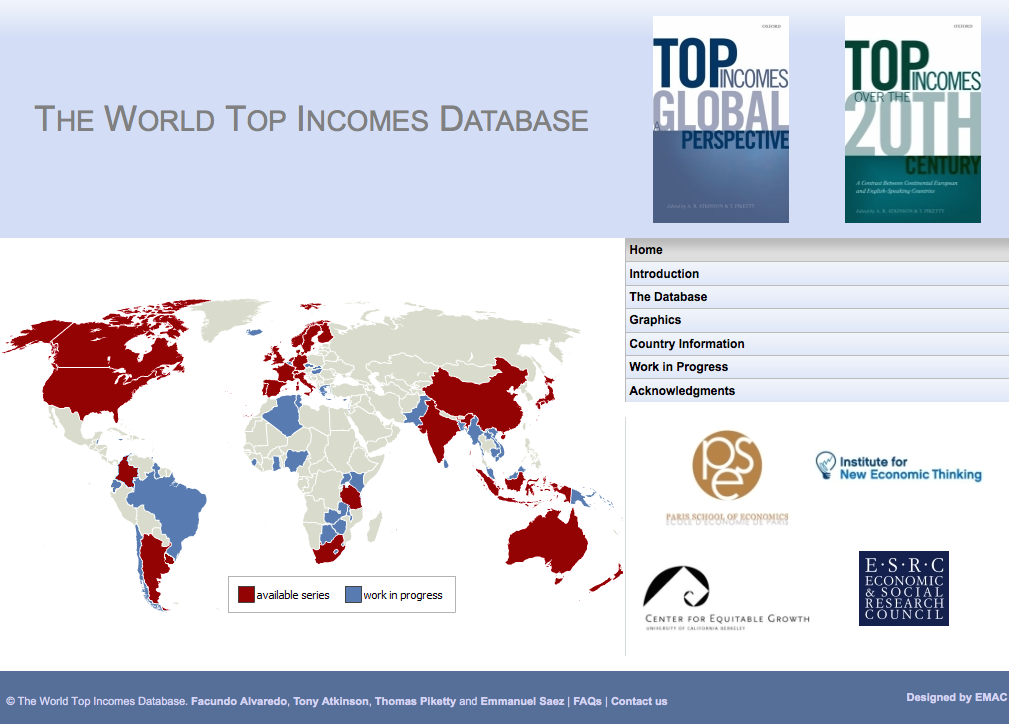
\includegraphics[width=0.9\textwidth]
{pictures/WorldTopIncomesDatabase}
\caption{\textbf{\url{http://topincomes.parisschoolofeconomics.eu}}}
\end{minipage}
\end{figure}
\end{frame}
%%%%%%%%%%%%%%%%%%%% Frame Here %%%%%%%%%%%%%%%%%%%%%%%%%%%%%%%%%%%%%%%%%%%%%%%%


%%%%%%%%%%%%%%%%%%%% Frame Here %%%%%%%%%%%%%%%%%%%%%%%%%%%%%%%%%%%%%%%%%%%%%%%%
\begin{frame}[label=Figure_0_1,fragile]
\frametitle{Figure I.1: Income inequality in the United States, 1910--2012}
\begin{figure}[t]
\begin{minipage}[b]{\textwidth}
\centering
\begin{knitrout}\footnotesize
\definecolor{shadecolor}{rgb}{0.969, 0.969, 0.969}\color{fgcolor}

{\centering 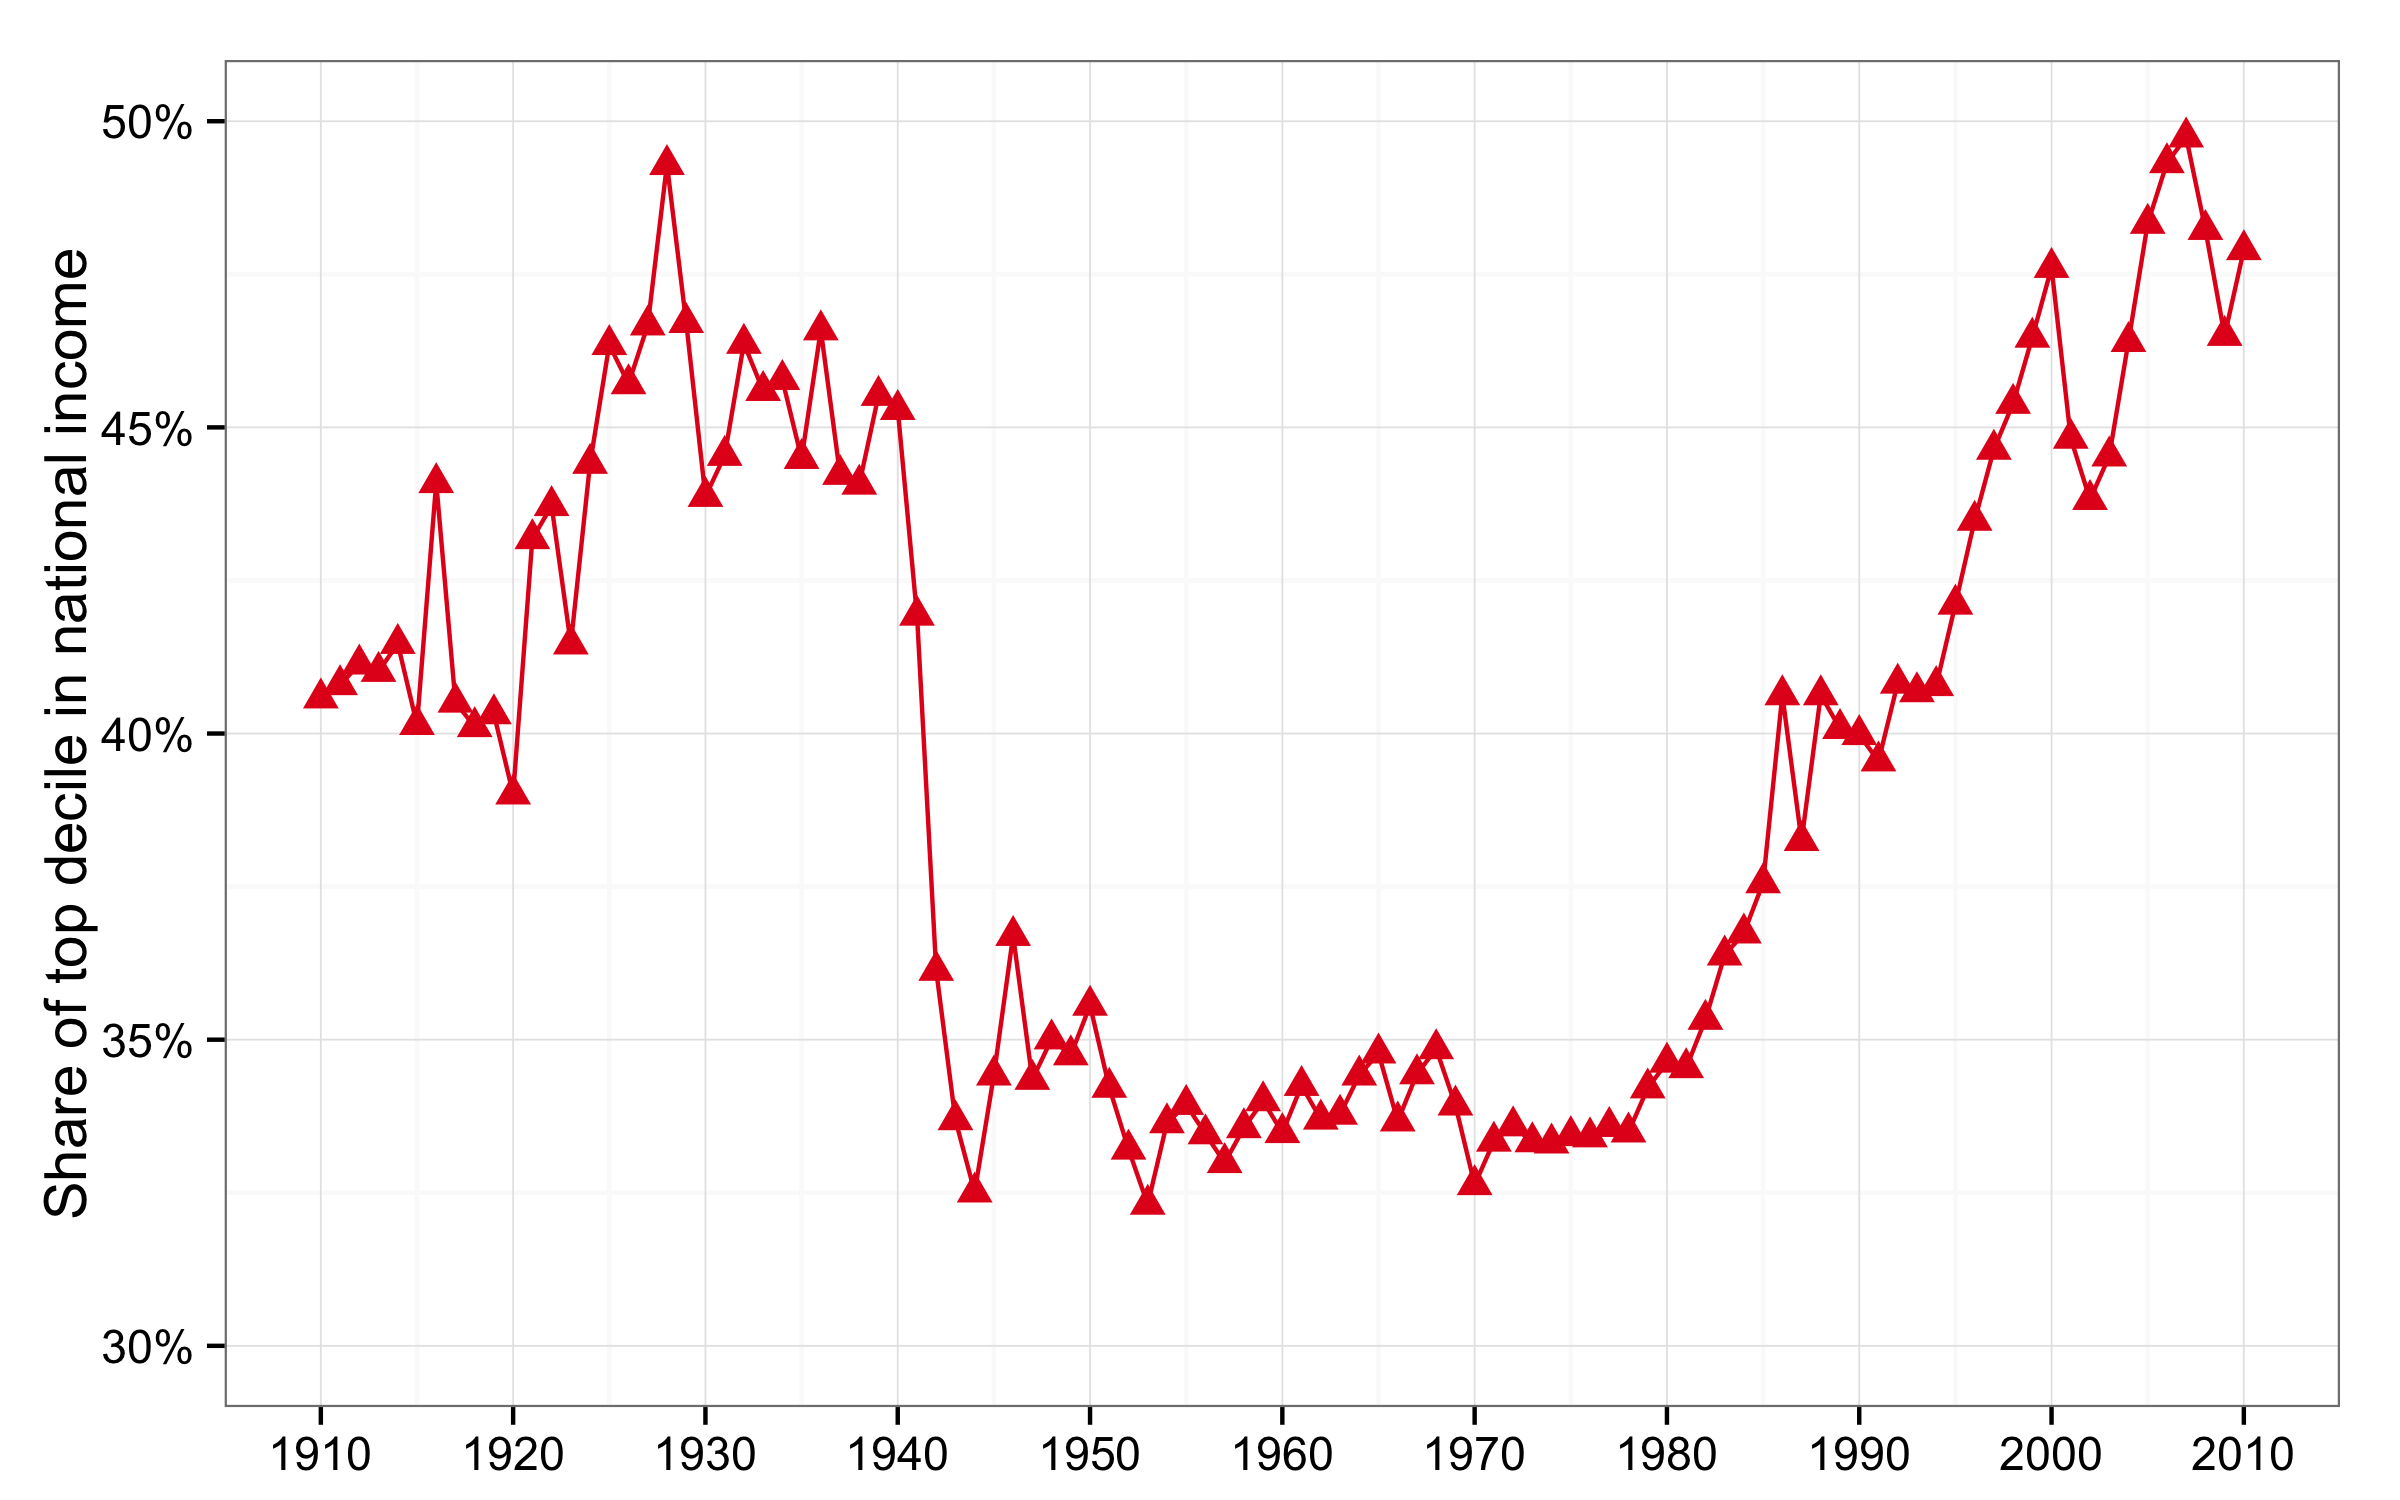
\includegraphics[width=1\linewidth]{figures/color/Figure_0_1} 

}



\end{knitrout}
\caption{The top decile share in U.S. national income dropped from 45--50\% in the 1910s--1920s to less than 35\% in the 1950s (this is the
1950 1960 fall documented by Kuznets); it then rose from less than 35\% in the 1970s to 45--50\% in the 2000s--2010s.}
\end{minipage}
\end{figure}
\end{frame}
%%%%%%%%%%%%%%%%%%%% Frame Here %%%%%%%%%%%%%%%%%%%%%%%%%%%%%%%%%%%%%%%%%%%%%%%%


%%%%%%%%%%%%%%%%%%%% Frame Here %%%%%%%%%%%%%%%%%%%%%%%%%%%%%%%%%%%%%%%%%%%%%%%%
\begin{frame}[label=Figure_0_2,fragile]
\frametitle{Figure I.2. The capital--income ratio in Europe, 1870--2012}
\begin{figure}[t]
\begin{minipage}[b]{\textwidth}
\centering
\begin{knitrout}\footnotesize
\definecolor{shadecolor}{rgb}{0.969, 0.969, 0.969}\color{fgcolor}

{\centering 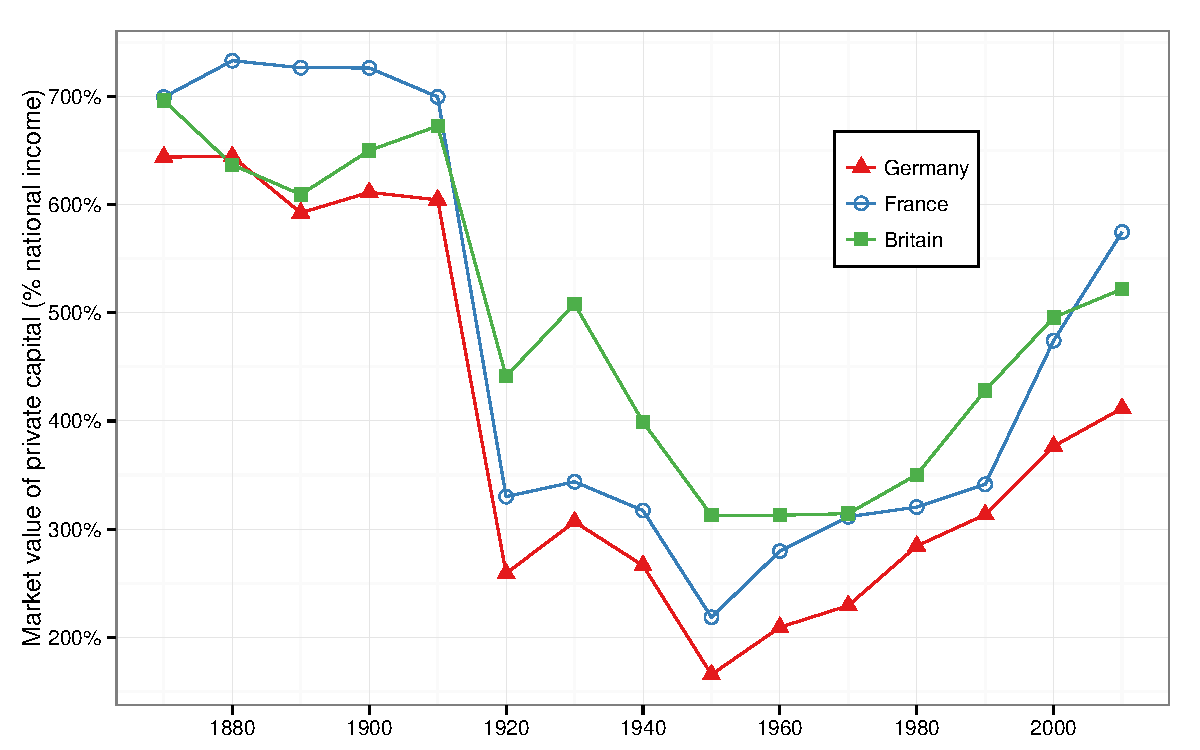
\includegraphics[width=1\linewidth]{figures/color/Figure_0_2} 

}



\end{knitrout}
\caption{Aggregate private wealth was worth about 6--7 years of national income in Europe in 1910, between 2 and 3 years in 1950, and between 4 and 6 years in 2010.}
\end{minipage}
\end{figure}
\end{frame}
%%%%%%%%%%%%%%%%%%%% Frame Here %%%%%%%%%%%%%%%%%%%%%%%%%%%%%%%%%%%%%%%%%%%%%%%%


%%%%%%%%%%%%%%%%%%%% Frame Here %%%%%%%%%%%%%%%%%%%%%%%%%%%%%%%%%%%%%%%%%%%%%%%%
\begin{frame}[label=Figure_8_1,fragile]
\frametitle{Figure 8.1. Income inequality in France, 1910--2010}
\begin{figure}[t]
\begin{minipage}[b]{\textwidth}
\centering
\begin{knitrout}\footnotesize
\definecolor{shadecolor}{rgb}{0.969, 0.969, 0.969}\color{fgcolor}

{\centering 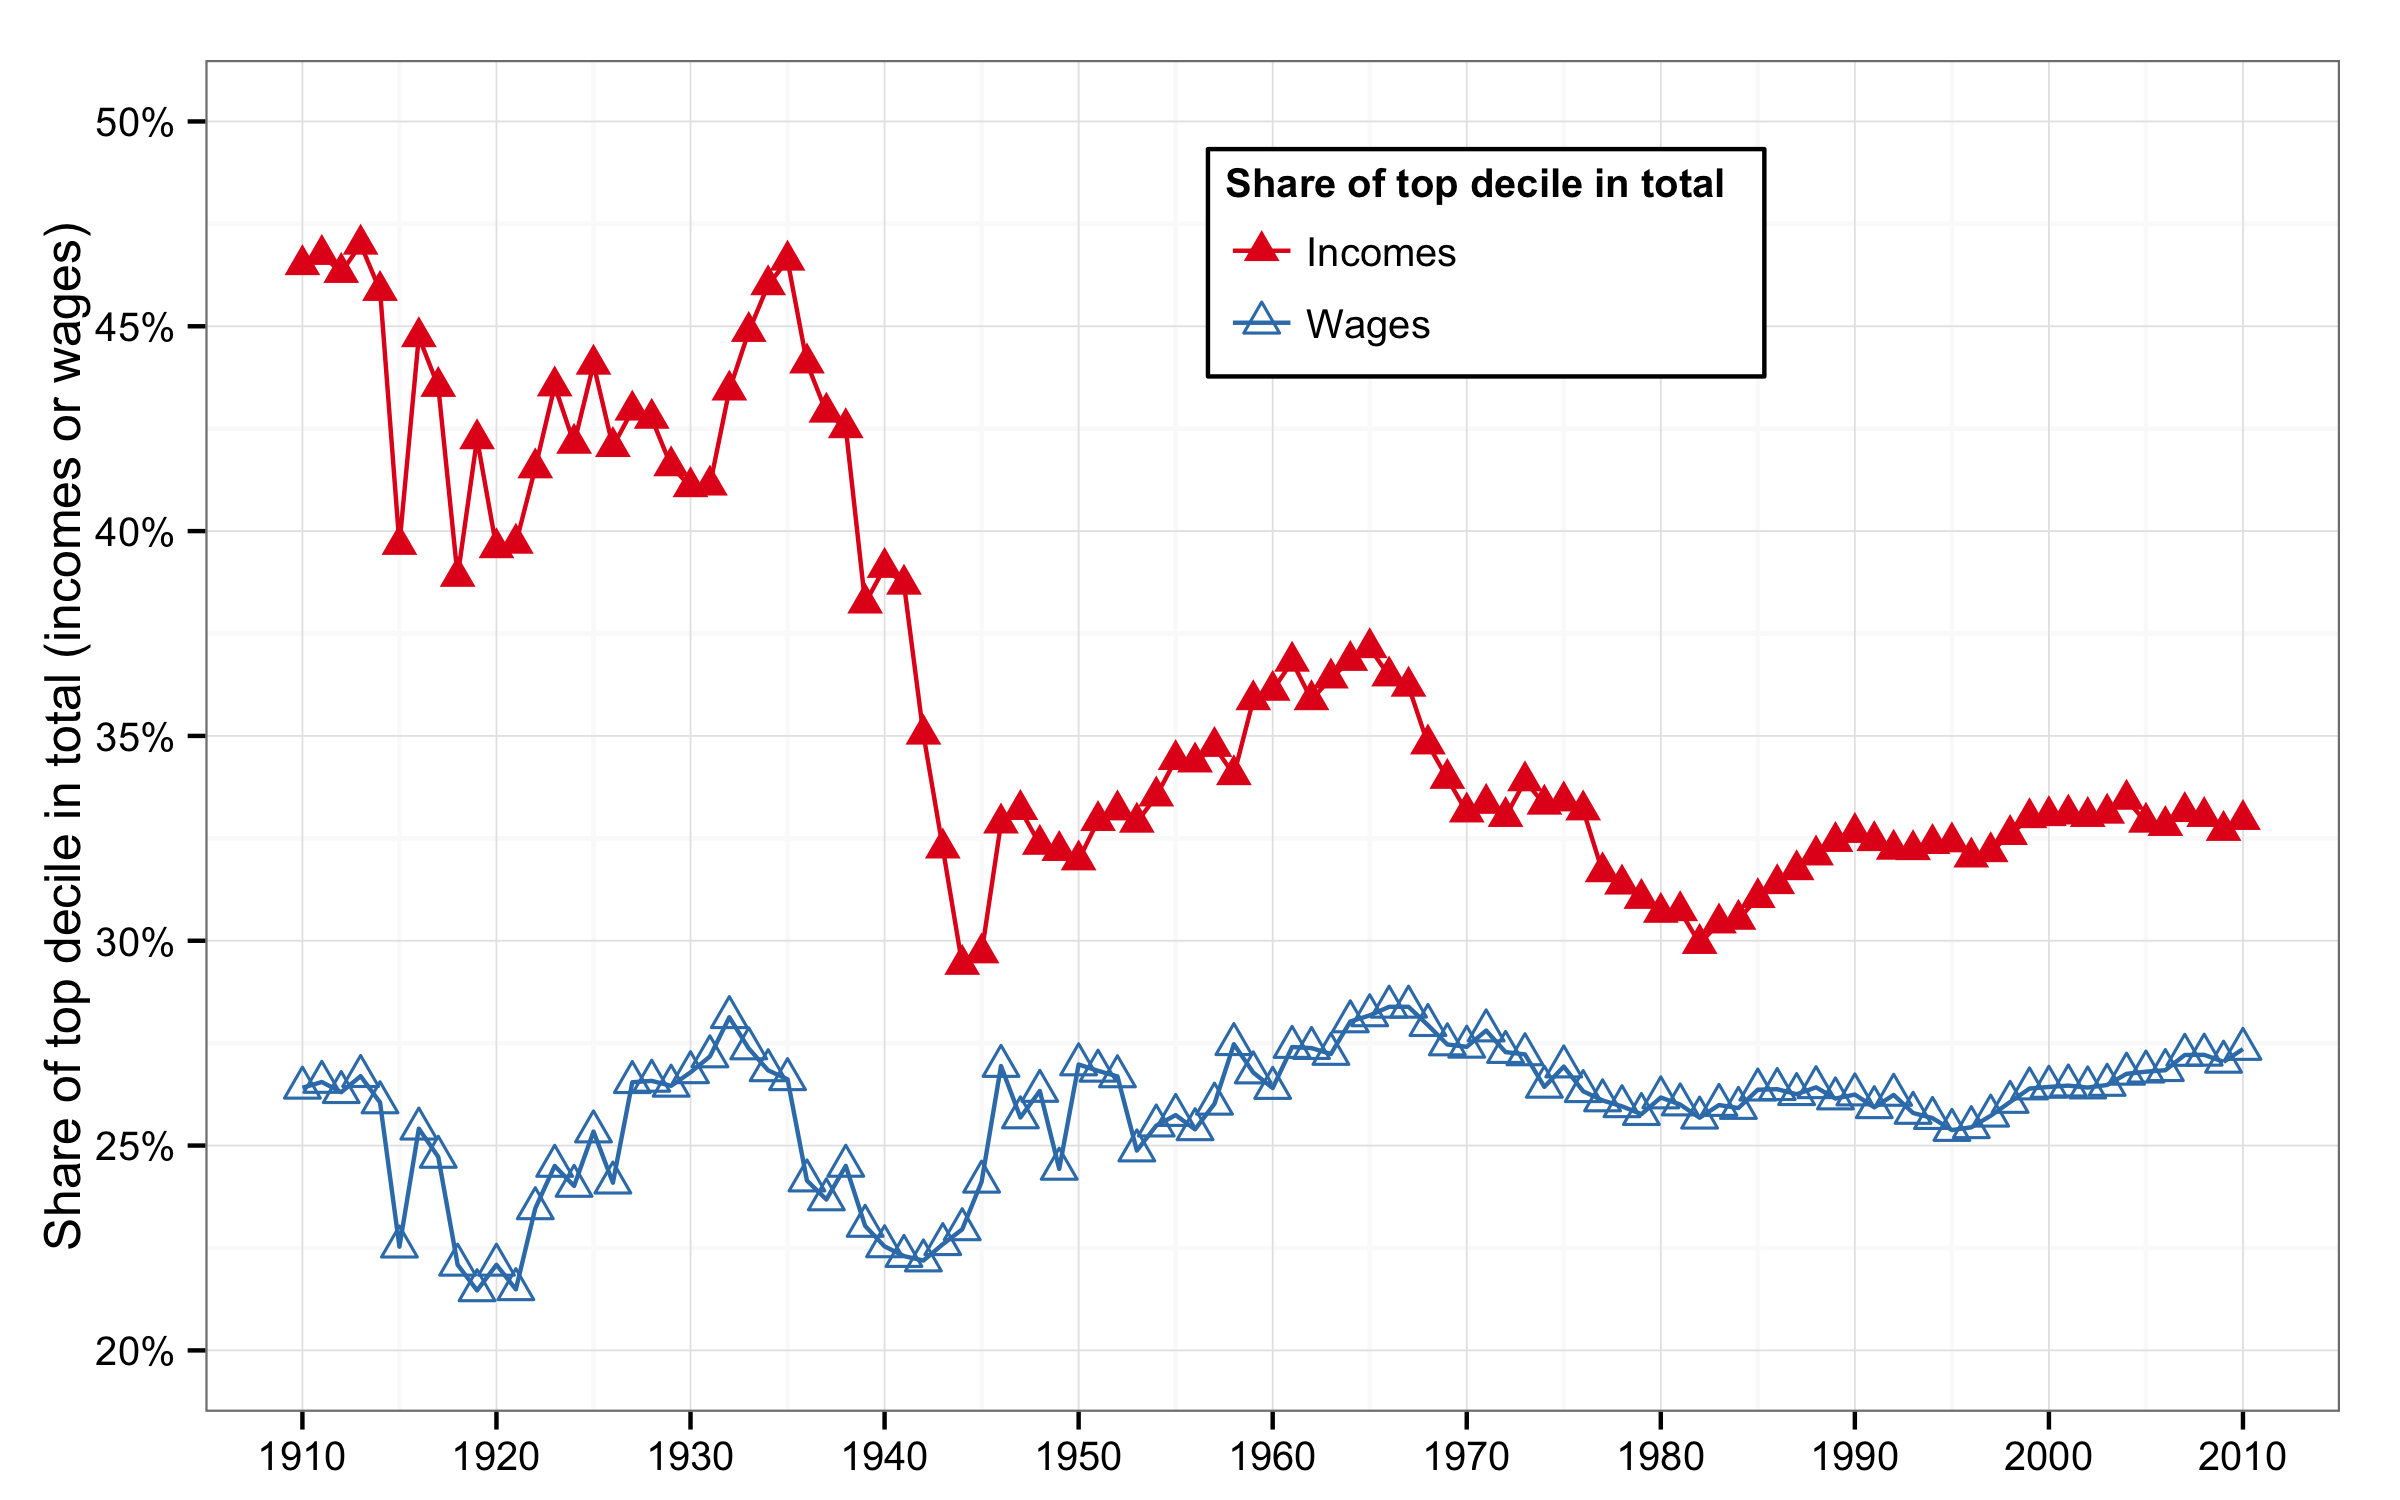
\includegraphics[width=1\linewidth]{figures/color/Figure_8_1} 

}



\end{knitrout}
\caption{Inequality of total income (labor and capital) has dropped in France during the twentieth century, while wage inequality has remained the same.}
\end{minipage}
\end{figure}
\end{frame}
%%%%%%%%%%%%%%%%%%%% Frame Here %%%%%%%%%%%%%%%%%%%%%%%%%%%%%%%%%%%%%%%%%%%%%%%%


%%%%%%%%%%%%%%%%%%%% Frame Here %%%%%%%%%%%%%%%%%%%%%%%%%%%%%%%%%%%%%%%%%%%%%%%%
\begin{frame}[label=Figure_8_2,fragile]
\frametitle{Figure 8.2. The fall of rentiers in France, 1910--2010}
\begin{figure}[t]
\begin{minipage}[b]{\textwidth}
\centering
\begin{knitrout}\footnotesize
\definecolor{shadecolor}{rgb}{0.969, 0.969, 0.969}\color{fgcolor}

{\centering 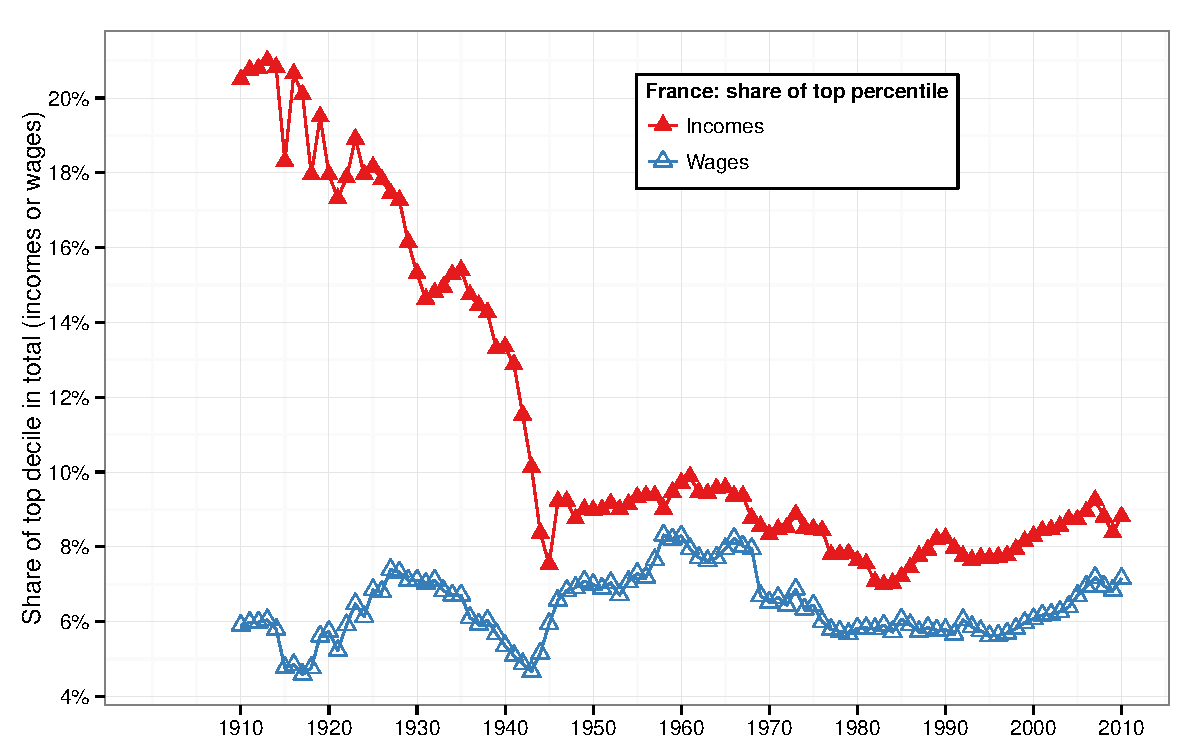
\includegraphics[width=1\linewidth]{figures/color/Figure_8_2} 

}



\end{knitrout}
\caption{The fall in the top percentile share (the top 1 percent highest incomes) in France between 1914 and 1945 is due to the fall of top capital incomes.}
\end{minipage}
\end{figure}
\end{frame}
%%%%%%%%%%%%%%%%%%%% Frame Here %%%%%%%%%%%%%%%%%%%%%%%%%%%%%%%%%%%%%%%%%%%%%%%%


%%%%%%%%%%%%%%%%%%%% Frame Here %%%%%%%%%%%%%%%%%%%%%%%%%%%%%%%%%%%%%%%%%%%%%%%%
\begin{frame}[label=Figure_8_3,fragile]
\frametitle{Figure 8.3. The composition of top incomes in France in 1932}
\begin{figure}[t]
\begin{minipage}[b]{\textwidth}
\centering
\begin{knitrout}\footnotesize
\definecolor{shadecolor}{rgb}{0.969, 0.969, 0.969}\color{fgcolor}

{\centering 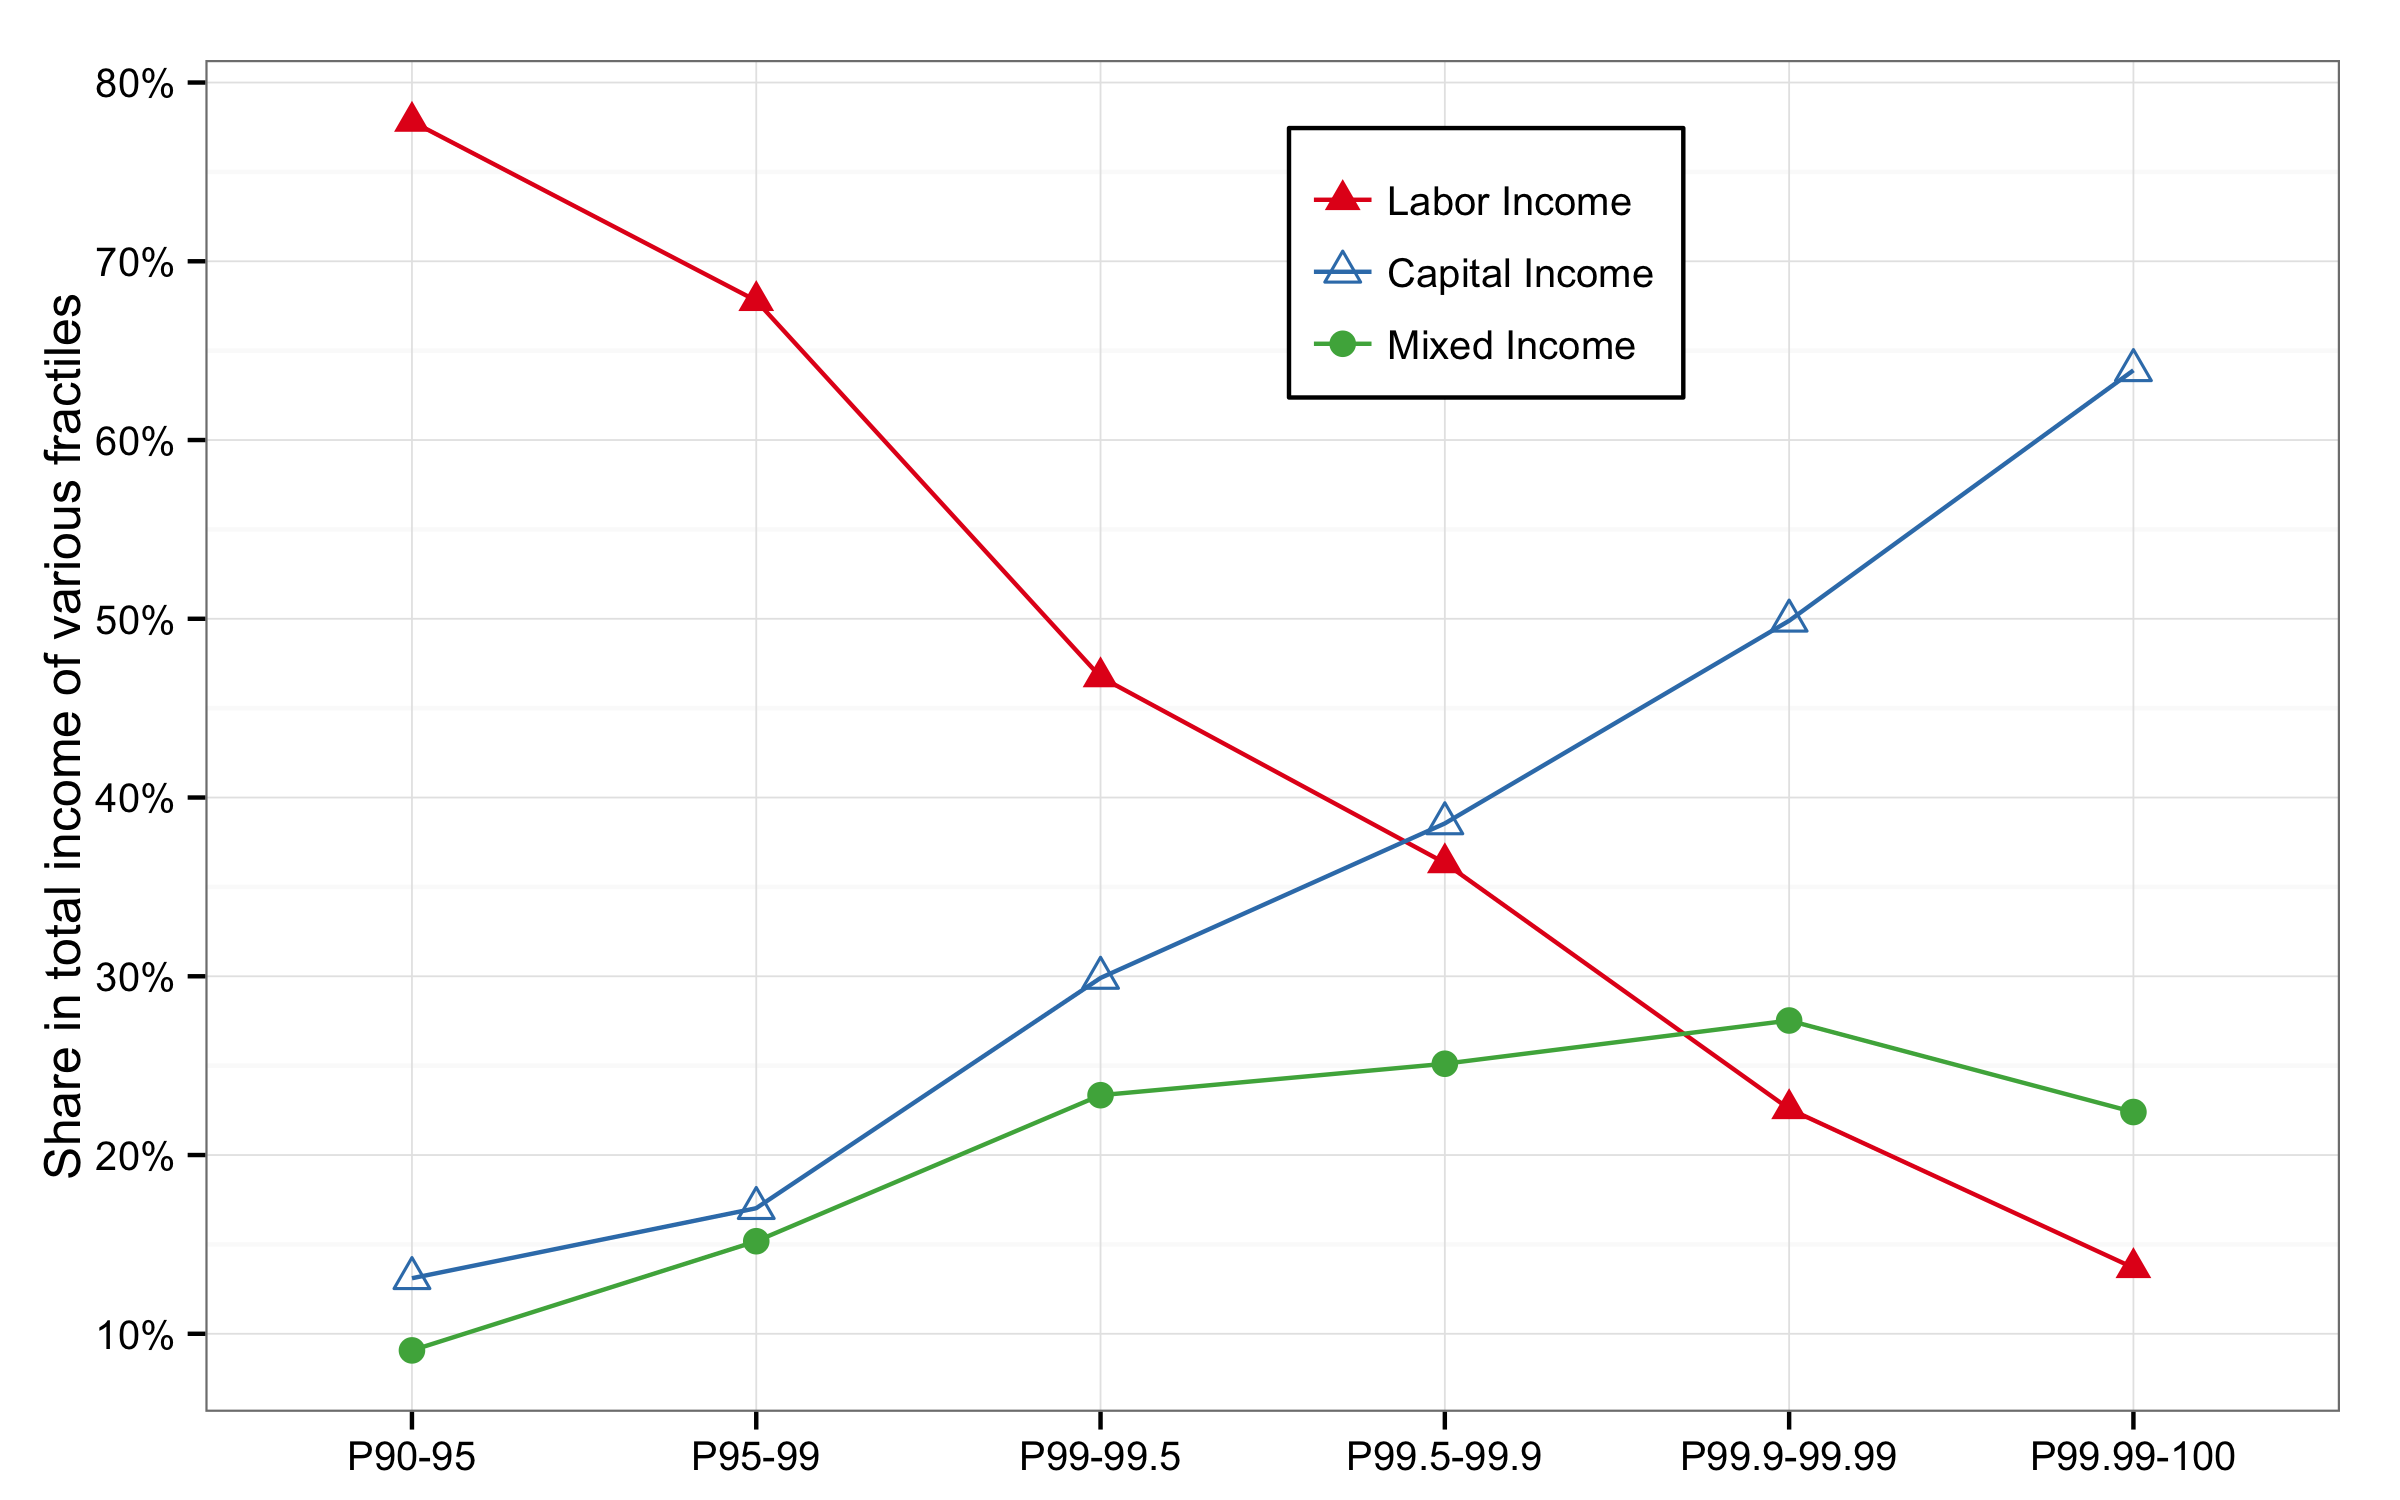
\includegraphics[width=1\linewidth]{figures/color/Figure_8_3} 

}



\end{knitrout}
\caption{Labor income becomes less and less important as one goes up within the top decile of total income. Notes: (i)~``P90--95'' includes individuals between percentiles 90 to 95, ``P95--99'' includes the next 4 percent, ``P99--99.5'' the next 0.5 percent, etc.; (ii)~Labor income: wages, bonuses, pensions. Capital income: dividends, interest, rent. Mixed income: self-employment income.}
\end{minipage}
\end{figure}
\end{frame}
%%%%%%%%%%%%%%%%%%%% Frame Here %%%%%%%%%%%%%%%%%%%%%%%%%%%%%%%%%%%%%%%%%%%%%%%%


%%%%%%%%%%%%%%%%%%%% Frame Here %%%%%%%%%%%%%%%%%%%%%%%%%%%%%%%%%%%%%%%%%%%%%%%%
\begin{frame}[label=Figure_8_4,fragile]
\frametitle{Figure 8.4. The composition of top incomes in France in 2005}
\begin{figure}[t]
\begin{minipage}[b]{\textwidth}
\centering
\begin{knitrout}\footnotesize
\definecolor{shadecolor}{rgb}{0.969, 0.969, 0.969}\color{fgcolor}

{\centering 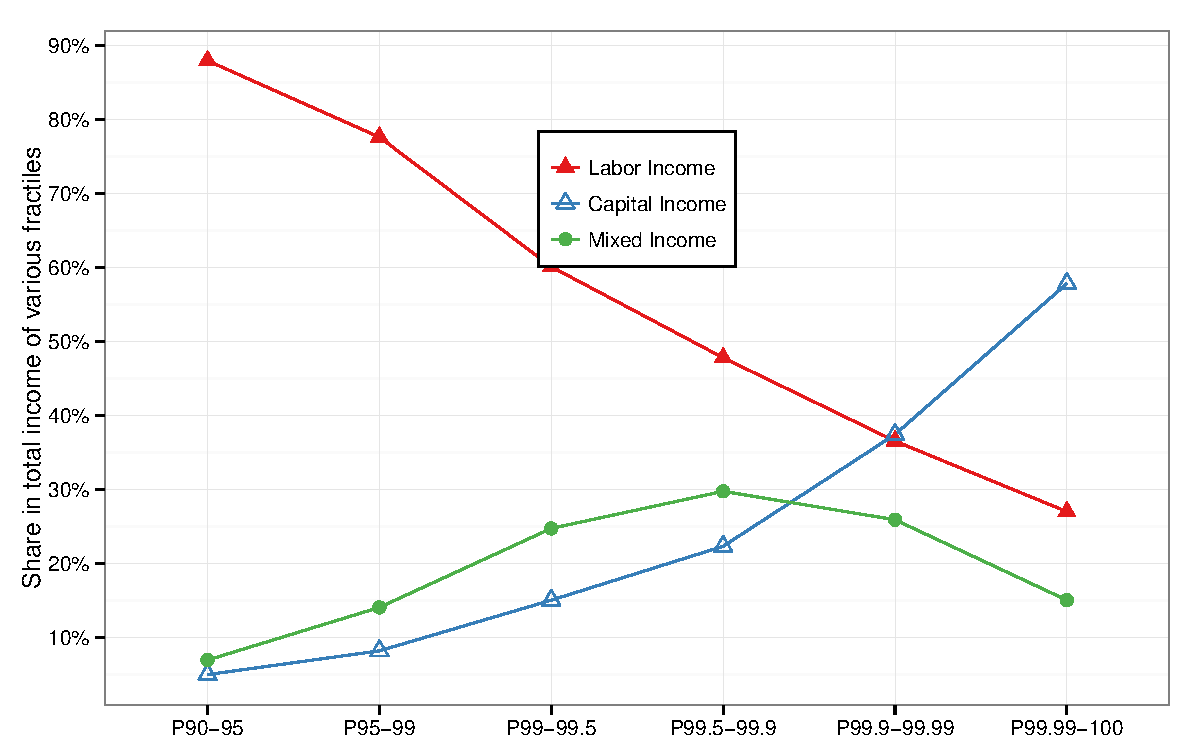
\includegraphics[width=1\linewidth]{figures/color/Figure_8_4} 

}



\end{knitrout}
\caption{Capital income becomes dominant at the level of the top 0.1 percent in France in 2005, as opposed to the top 0.5 percent in 1932.}
\end{minipage}
\end{figure}
\end{frame}
%%%%%%%%%%%%%%%%%%%% Frame Here %%%%%%%%%%%%%%%%%%%%%%%%%%%%%%%%%%%%%%%%%%%%%%%%


%%%%%%%%%%%%%%%%%%%% Frame Here %%%%%%%%%%%%%%%%%%%%%%%%%%%%%%%%%%%%%%%%%%%%%%%%
\begin{frame}[label=Figure_8_5,fragile]
\frametitle{Figure 8.5. Income inequality in the United States, 1910--2010}
\begin{figure}[t]
\begin{minipage}[b]{\textwidth}
\centering
\begin{knitrout}\footnotesize
\definecolor{shadecolor}{rgb}{0.969, 0.969, 0.969}\color{fgcolor}

{\centering 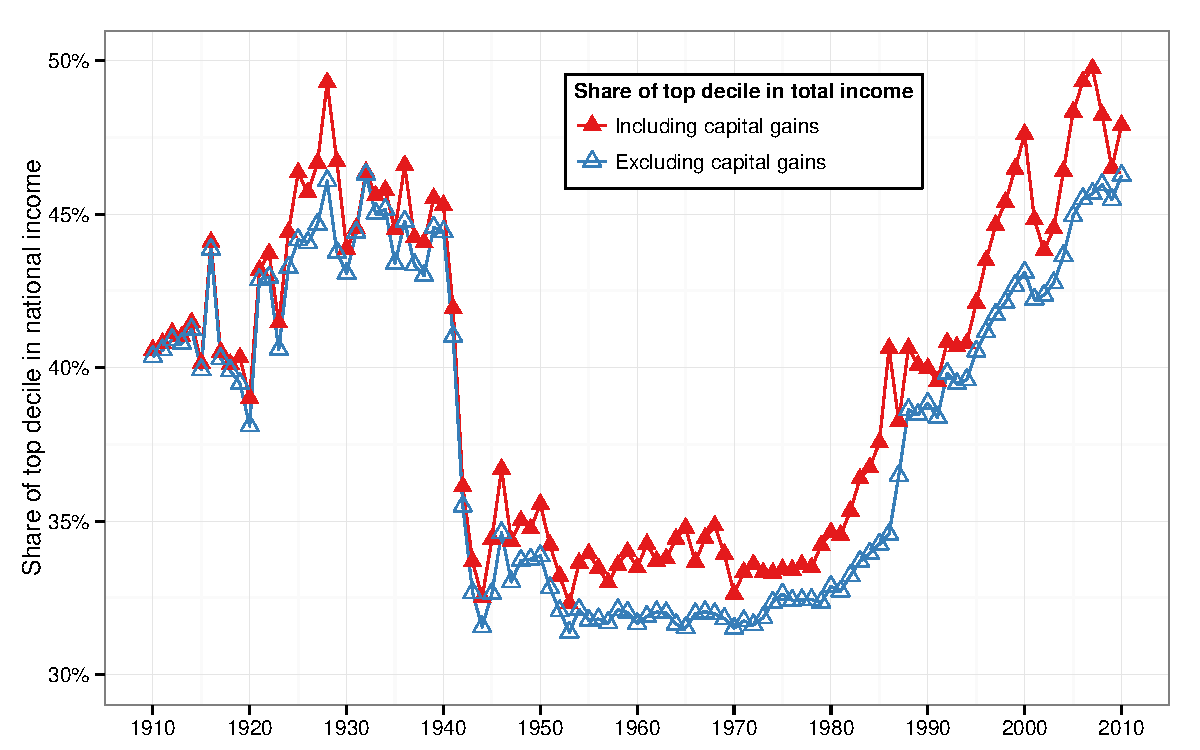
\includegraphics[width=1\linewidth]{figures/color/Figure_8_5} 

}



\end{knitrout}
\caption{The top decile share in U.S. national income dropped from 45--50\% in the 1910s--1920s to less than 35\% in the 1950s (this is the
1950 1960 fall documented by Kuznets); it then rose from less than 35\% in the 1970s to 45--50\% in the 2000s--2010s.}
\end{minipage}
\end{figure}
\end{frame}
%%%%%%%%%%%%%%%%%%%% Frame Here %%%%%%%%%%%%%%%%%%%%%%%%%%%%%%%%%%%%%%%%%%%%%%%%


%%%%%%%%%%%%%%%%%%%% Frame Here %%%%%%%%%%%%%%%%%%%%%%%%%%%%%%%%%%%%%%%%%%%%%%%%
\begin{frame}[label=Figure_8_6,fragile]
\frametitle{Figure 8.6. Decomposition of the top decile, United States, 1910--2010}
\begin{figure}[t]
\begin{minipage}[b]{\textwidth}
\centering
\begin{knitrout}\footnotesize
\definecolor{shadecolor}{rgb}{0.969, 0.969, 0.969}\color{fgcolor}

{\centering 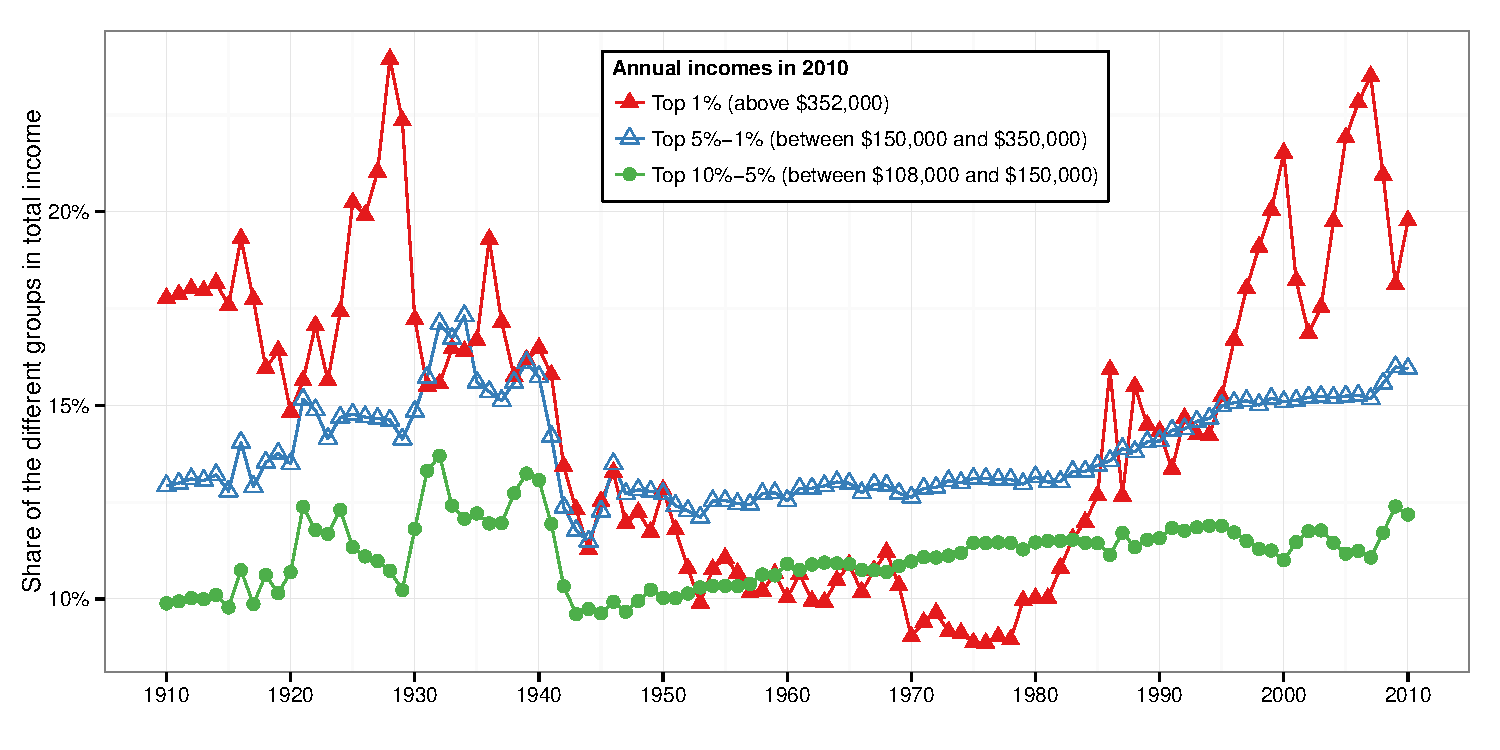
\includegraphics[width=1\linewidth]{figures/color/Figure_8_6} 

}



\end{knitrout}
\caption{The rise of the top decile income share since the 1970s is mostly due to the top percentile.}
\end{minipage}
\end{figure}
\end{frame}
%%%%%%%%%%%%%%%%%%%% Frame Here %%%%%%%%%%%%%%%%%%%%%%%%%%%%%%%%%%%%%%%%%%%%%%%%


%%%%%%%%%%%%%%%%%%%% Frame Here %%%%%%%%%%%%%%%%%%%%%%%%%%%%%%%%%%%%%%%%%%%%%%%%
\begin{frame}[label=Figure_8_7,fragile]
\frametitle{Figure 8.7. High incomes and high wages in the United States, 1910--2010}
\begin{figure}[t]
\begin{minipage}[b]{\textwidth}
\centering % To Do: add 'excluding capital gains'
\begin{knitrout}\footnotesize
\definecolor{shadecolor}{rgb}{0.969, 0.969, 0.969}\color{fgcolor}

{\centering 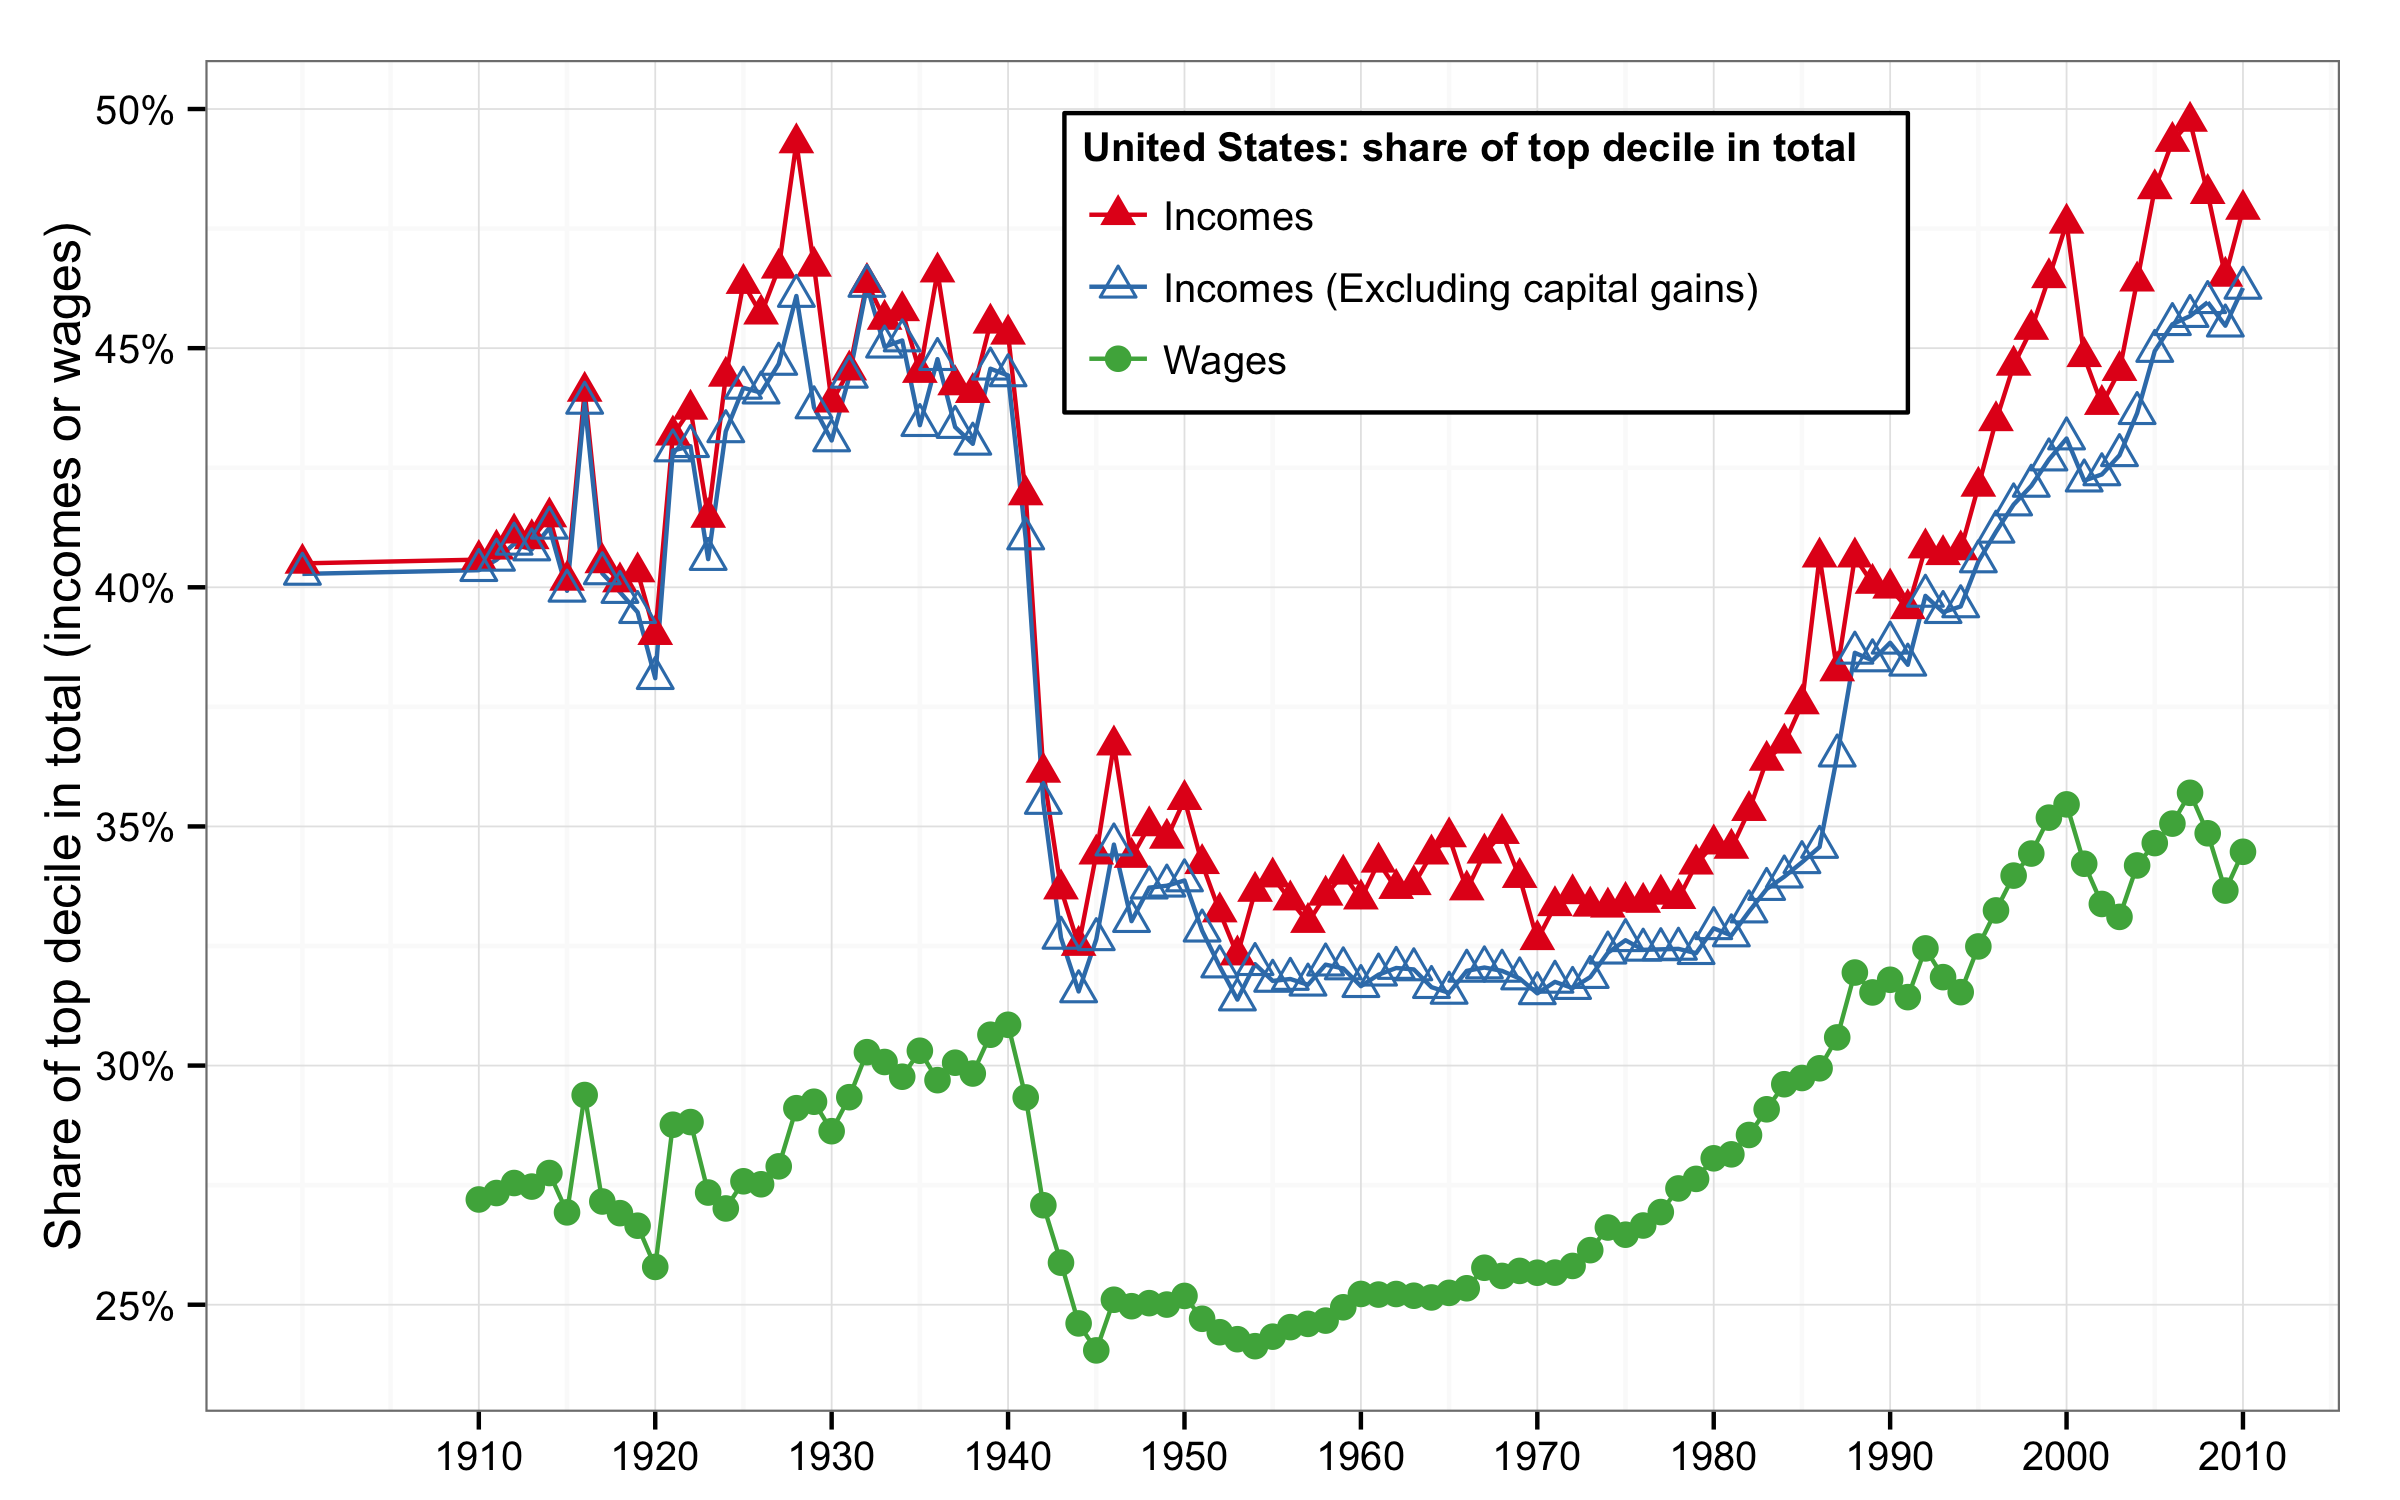
\includegraphics[width=1\linewidth]{figures/color/Figure_8_7} 

}



\end{knitrout}
\caption{The rise of income inequality since the 1970s is largely due to the rise of wage inequality.}
\end{minipage}
\end{figure}
\end{frame}
%%%%%%%%%%%%%%%%%%%% Frame Here %%%%%%%%%%%%%%%%%%%%%%%%%%%%%%%%%%%%%%%%%%%%%%%%


%%%%%%%%%%%%%%%%%%%% Frame Here %%%%%%%%%%%%%%%%%%%%%%%%%%%%%%%%%%%%%%%%%%%%%%%%
\begin{frame}[label=Figure_8_8,fragile]
\frametitle{Figure 8.8. The transformation of the top 1 percent in the United States, 1910--2010}
\begin{figure}[t]
\begin{minipage}[b]{\textwidth}
\centering % To Do: add 'excluding capital gains'
\begin{knitrout}\footnotesize
\definecolor{shadecolor}{rgb}{0.969, 0.969, 0.969}\color{fgcolor}

{\centering 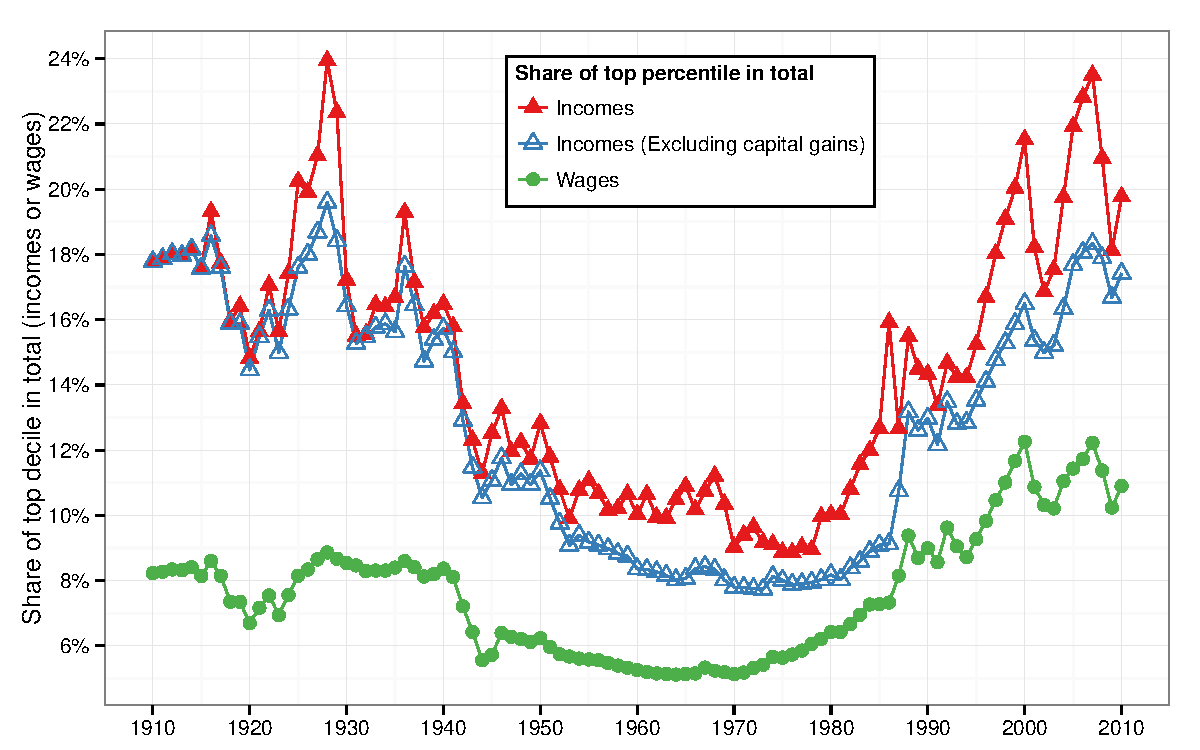
\includegraphics[width=1\linewidth]{figures/color/Figure_8_8} 

}



\end{knitrout}
\caption{The rise in the top 1 percent highest incomes since the 1970s is largely due to the rise in the top 1 percent highest wages.}
\end{minipage}
\end{figure}
\end{frame}
%%%%%%%%%%%%%%%%%%%% Frame Here %%%%%%%%%%%%%%%%%%%%%%%%%%%%%%%%%%%%%%%%%%%%%%%%


%%%%%%%%%%%%%%%%%%%% Frame Here %%%%%%%%%%%%%%%%%%%%%%%%%%%%%%%%%%%%%%%%%%%%%%%%
\begin{frame}[label=Figure_8_9,fragile]
\frametitle{Figure 8.9. The composition of top incomes in the United States in 1929}
\begin{figure}[t]
\begin{minipage}[b]{\textwidth}
\centering
\begin{knitrout}\footnotesize
\definecolor{shadecolor}{rgb}{0.969, 0.969, 0.969}\color{fgcolor}

{\centering 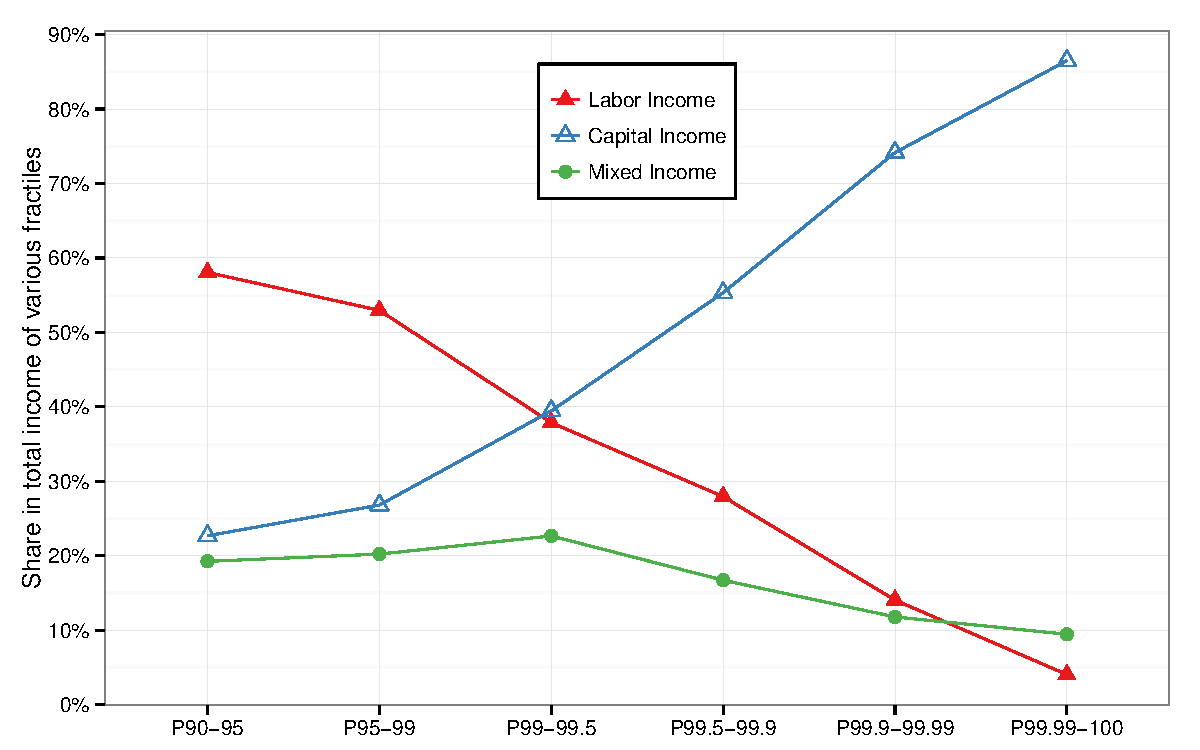
\includegraphics[width=1\linewidth]{figures/color/Figure_8_9} 

}



\end{knitrout}
\caption{Labor income becomes less and less important as one moves up within the top income decile.}
\end{minipage}
\end{figure}
\end{frame}
%%%%%%%%%%%%%%%%%%%% Frame Here %%%%%%%%%%%%%%%%%%%%%%%%%%%%%%%%%%%%%%%%%%%%%%%%


%%%%%%%%%%%%%%%%%%%% Frame Here %%%%%%%%%%%%%%%%%%%%%%%%%%%%%%%%%%%%%%%%%%%%%%%%
\begin{frame}[label=Figure_8_10,fragile]
\frametitle{Figure 8.10. The composition of top incomes in the United States in 2007}
\begin{figure}[t]
\begin{minipage}[b]{\textwidth}
\centering
\begin{knitrout}\footnotesize
\definecolor{shadecolor}{rgb}{0.969, 0.969, 0.969}\color{fgcolor}

{\centering 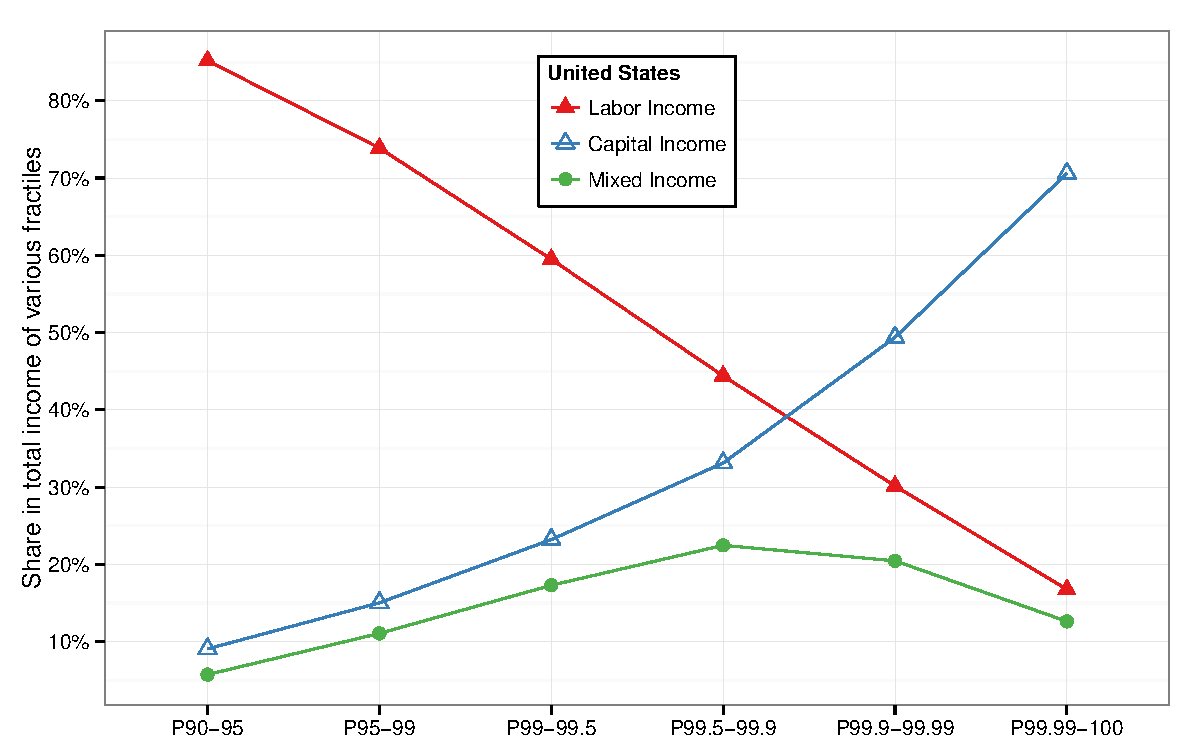
\includegraphics[width=1\linewidth]{figures/color/Figure_8_10} 

}



\end{knitrout}
\caption{Capital income becomes dominant at the level of top 0.1 percent in 2007, as opposed to the top 1 percent in 1929.}
\end{minipage}
\end{figure}
\end{frame}
%%%%%%%%%%%%%%%%%%%% Frame Here %%%%%%%%%%%%%%%%%%%%%%%%%%%%%%%%%%%%%%%%%%%%%%%%


%%%%%%%%%%%%%%%%%%%% Frame Here %%%%%%%%%%%%%%%%%%%%%%%%%%%%%%%%%%%%%%%%%%%%%%%%
\begin{frame}[label=ThreePoints,fragile,shrink=4]
\frametitle{This presentation: three points}
\begin{enumerate}
\item
\textbf{The return of a patrimonial (or wealth-based) society} in the Old World (Europe, Japan). Wealth-income ratios seem to be returning to very high levels in low growth countries.
\medskip\newline
Intuition: in a slow-growth society, wealth accumulated in the past can naturally become very important. In the very long run, this can be relevant for the entire world.
\item 
\textbf{The future of wealth concentration}: with high $r-g$ during 21c ($r =$~`net-of-tax rate of return', $g =$~`growth rate'), then wealth inequality might reach or surpass 19c oligarchic levels; conversely, suitable institutions can allow to democratize wealth.
\item
\textbf{Inequality in America} (``meritocratic extremism''): is the New World developing a new inequality model that is based upon extreme labor income inequality more than upon wealth inequality? Is it more merit-based, or can it become the worst of all worlds?
\end{enumerate}
\end{frame}
%%%%%%%%%%%%%%%%%%%% Frame Here %%%%%%%%%%%%%%%%%%%%%%%%%%%%%%%%%%%%%%%%%%%%%%%%


%%%%%%%%%%%%%%%%%%%% Frame Here %%%%%%%%%%%%%%%%%%%%%%%%%%%%%%%%%%%%%%%%%%%%%%%%
\begin{frame}[label=BrasilVersus]
\frametitle{Brasil vs Europe--US--Japan}
\begin{itemize}
\item
\textbf{Top income shares}: income inequality is known to be high in Brasil; but it is probably underestimated (problem with household surveys); little access to fiscal data in Brasil.
\item 
\textbf{Wealth-income ratios}: probably a strong rise in Brasil (real estate prices), but we do not really know.
\item
\textbf{Wealth inequality}: probably very high, but we do not really know; no access to property tax and inheritance tax statistics.
\item
\textbf{Like other countries, Brasil needs more transparency about income and wealth}; progressive tax on income, inheritance and wealth would be a powerful way to produce information about how the different income and wealth groups are benefiting from growth.
\end{itemize}
\end{frame}
%%%%%%%%%%%%%%%%%%%% Frame Here %%%%%%%%%%%%%%%%%%%%%%%%%%%%%%%%%%%%%%%%%%%%%%%%


%%%%%%%%%%%%%%%%%%%% Frame Here %%%%%%%%%%%%%%%%%%%%%%%%%%%%%%%%%%%%%%%%%%%%%%%%
\begin{frame}[label=BrazilUSTop1]
\frametitle{Top 1\% income share: Brazil and United States, 2006--2012}
\begin{figure}[t]
\begin{minipage}[b]{\textwidth}
\centering
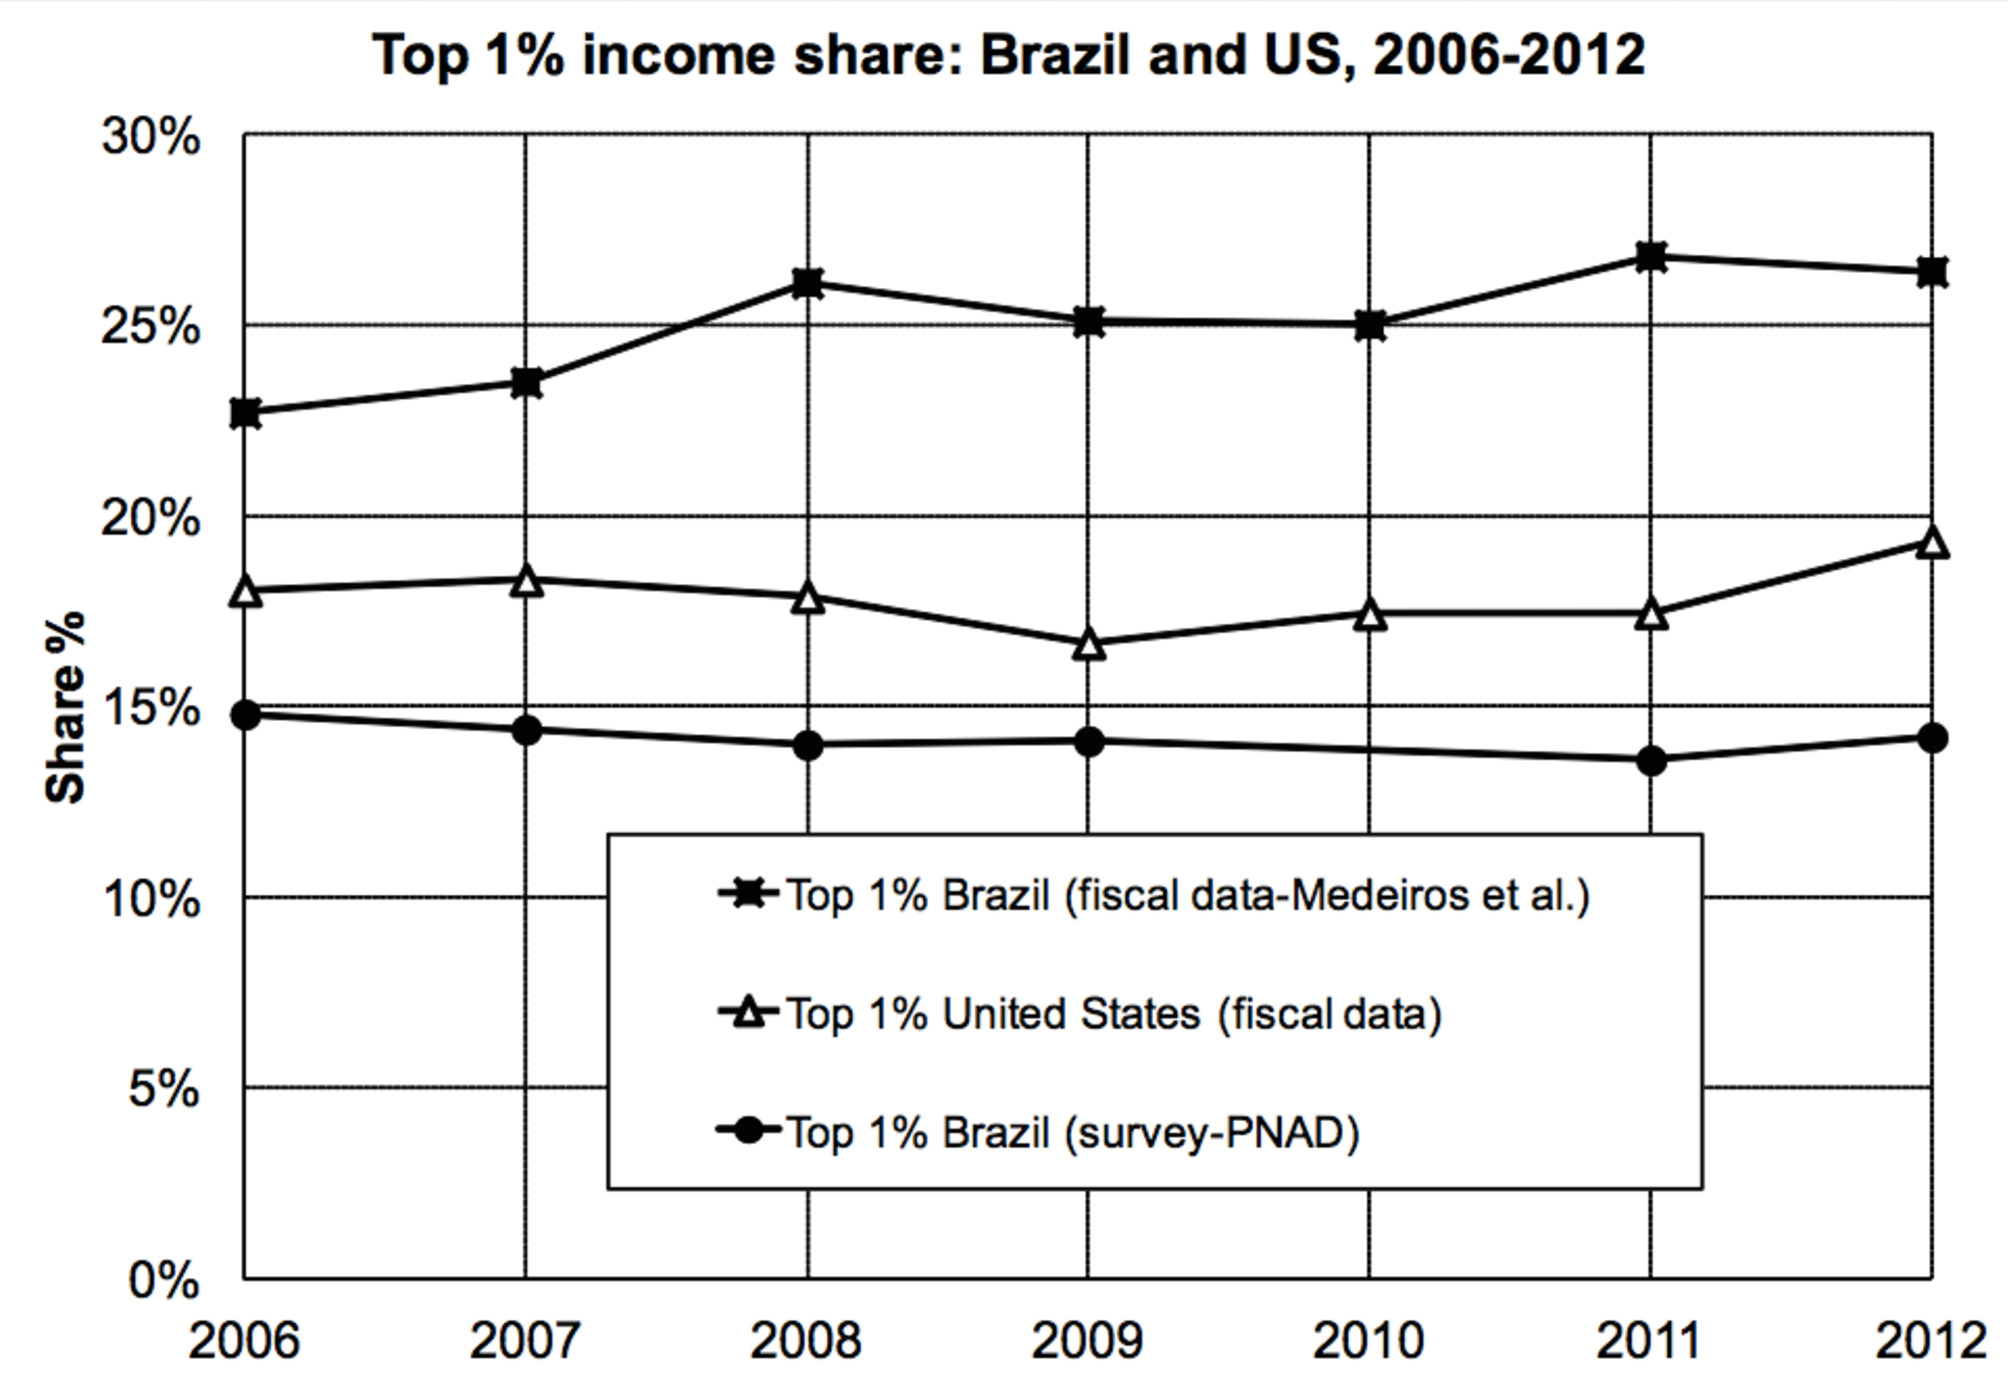
\includegraphics[width=\textwidth]
{pictures/Top1BrazilVsUSA}
\caption{To Do: Get Data to Recreate Figure}
\end{minipage}
\end{figure}
\end{frame}
%%%%%%%%%%%%%%%%%%%% Frame Here %%%%%%%%%%%%%%%%%%%%%%%%%%%%%%%%%%%%%%%%%%%%%%%%


%%%%%%%%%%%%%%%%%%%% Frame Here %%%%%%%%%%%%%%%%%%%%%%%%%%%%%%%%%%%%%%%%%%%%%%%%
\begin{frame}[label=BrazilUSTop10]
\frametitle{Top 10\% income share: Brazil and United States, 2006--2012}
\begin{figure}[t]
\begin{minipage}[b]{\textwidth}
\centering
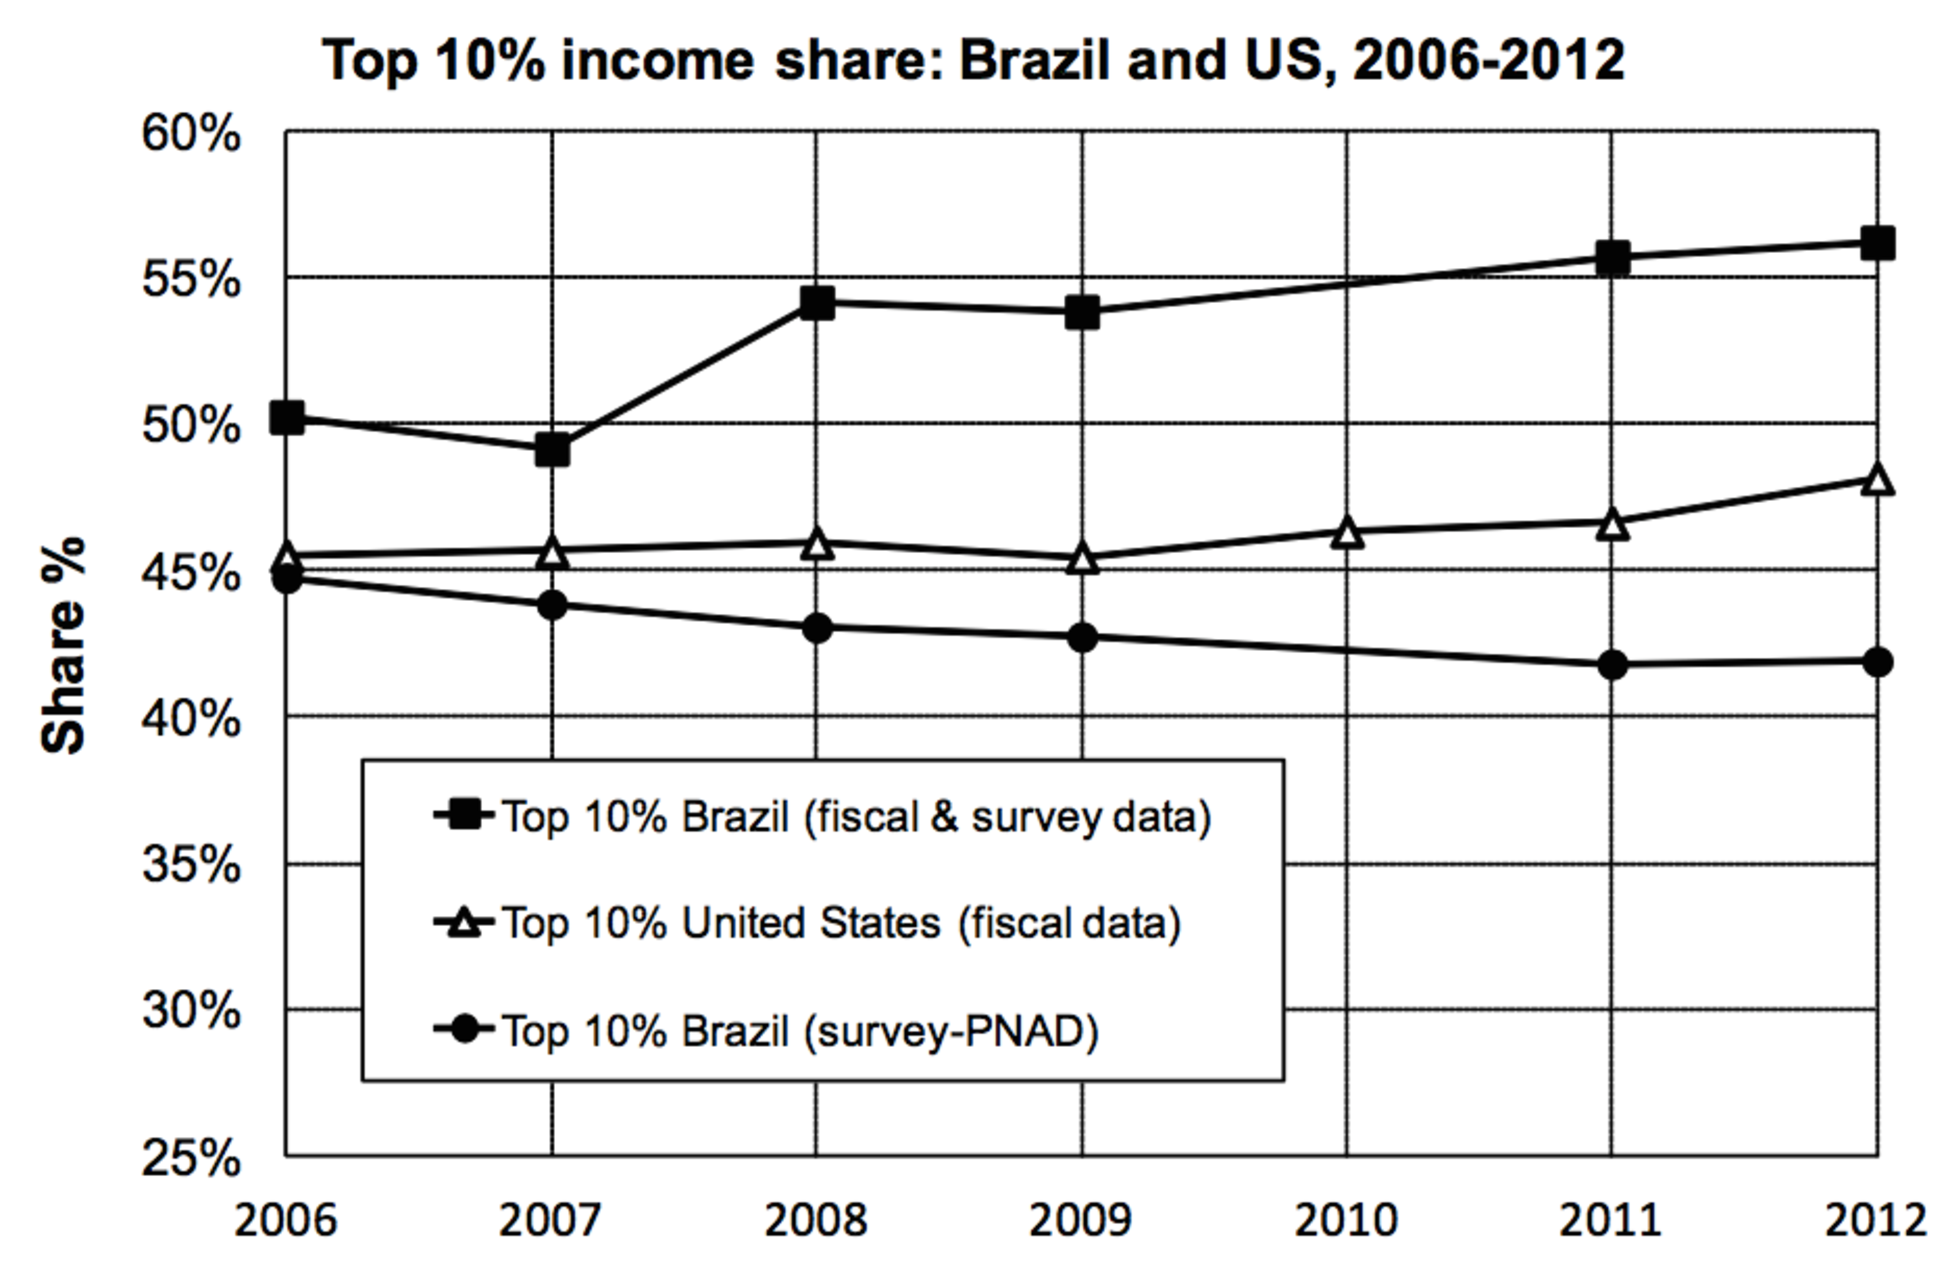
\includegraphics[width=\textwidth]
{pictures/Top10BrazilVsUSA}
\caption{To Do: Get Data to Recreate Figure}
\end{minipage}
\end{figure}
\end{frame}
%%%%%%%%%%%%%%%%%%%% Frame Here %%%%%%%%%%%%%%%%%%%%%%%%%%%%%%%%%%%%%%%%%%%%%%%%


%%%%%%%%%%%%%%%%%%%% Frame Here %%%%%%%%%%%%%%%%%%%%%%%%%%%%%%%%%%%%%%%%%%%%%%%%
\begin{frame}[label=BrazilInequality]
\frametitle{Income Inequality in Brazil: 1976--2013}
\begin{figure}[t]
\begin{minipage}[b]{\textwidth}
\centering
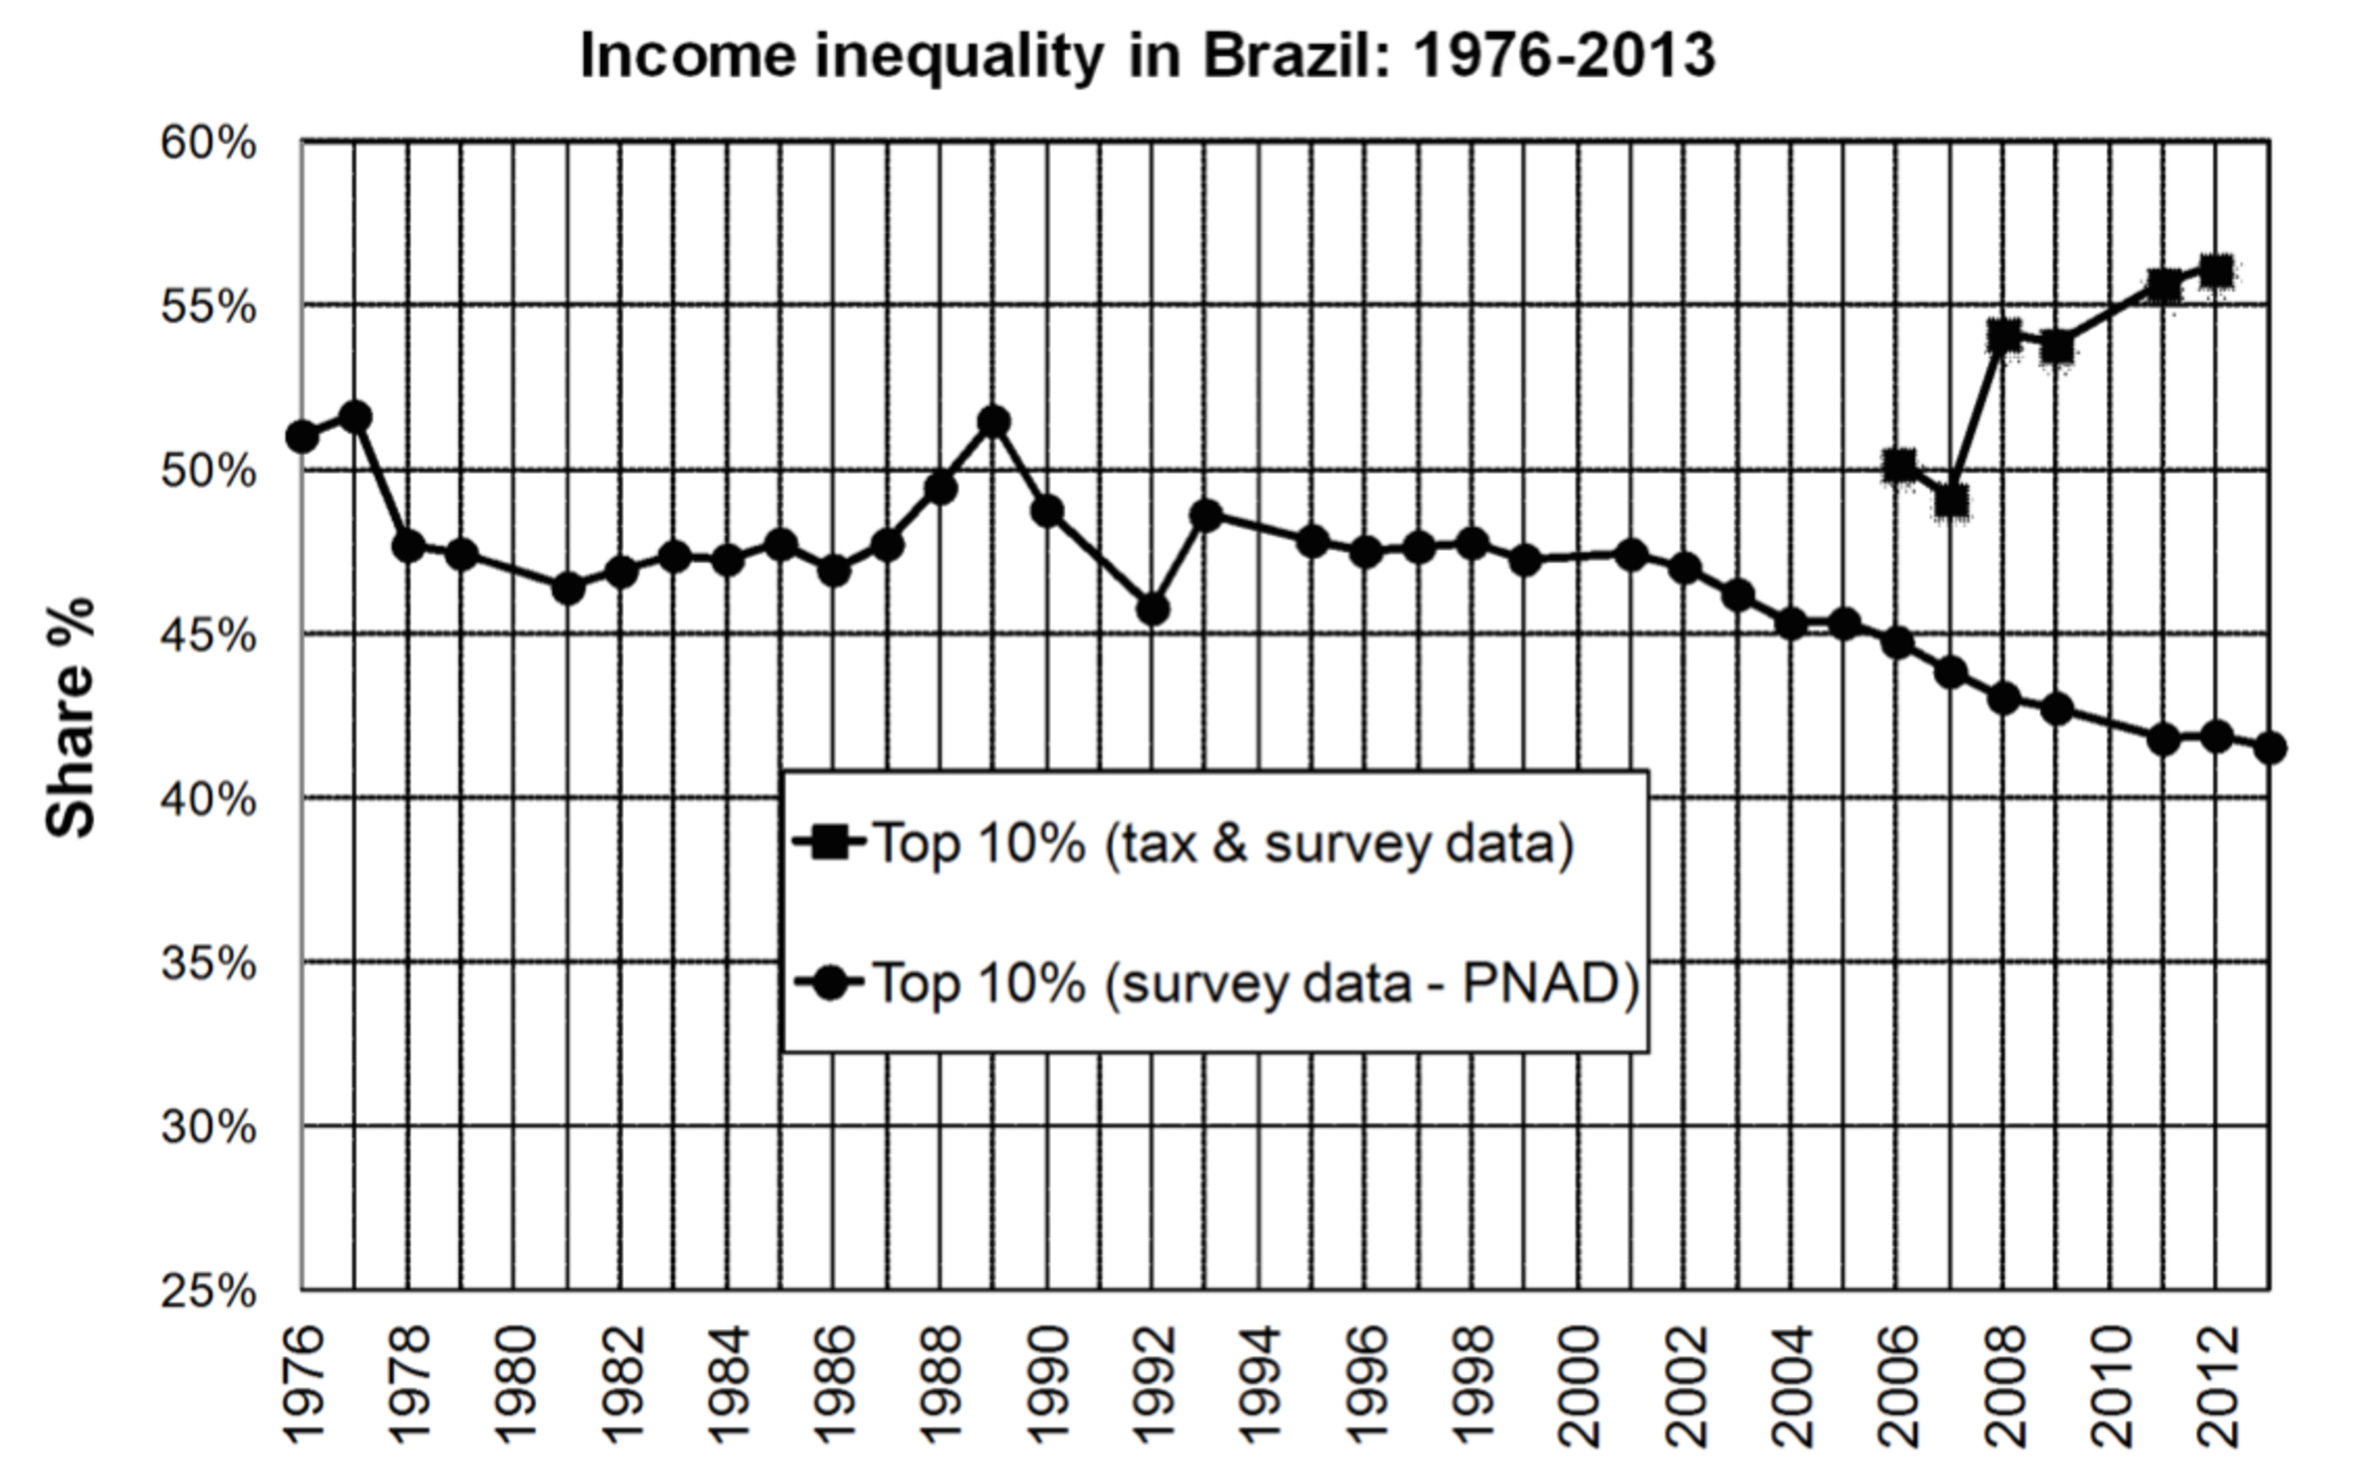
\includegraphics[width=\textwidth]
{pictures/IncomeInequalityBrazil}
\caption{To Do: Get Data to Recreate Figure}
\end{minipage}
\end{figure}
\end{frame}
%%%%%%%%%%%%%%%%%%%% Frame Here %%%%%%%%%%%%%%%%%%%%%%%%%%%%%%%%%%%%%%%%%%%%%%%%


\againframe[shrink=4]{ThreePoints}

\againframe{Figure_0_2}

%%%%%%%%%%%%%%%%%%%% Frame Here %%%%%%%%%%%%%%%%%%%%%%%%%%%%%%%%%%%%%%%%%%%%%%%%
\begin{frame}[label=Figure_5_1]
\frametitle{Figure 5.1: Private \& public capital in Europe \& United States, 1870--2010}
\begin{figure}[t]
\begin{minipage}[b]{\textwidth}
\centering
\begin{knitrout}\footnotesize
\definecolor{shadecolor}{rgb}{0.969, 0.969, 0.969}\color{fgcolor}

{\centering 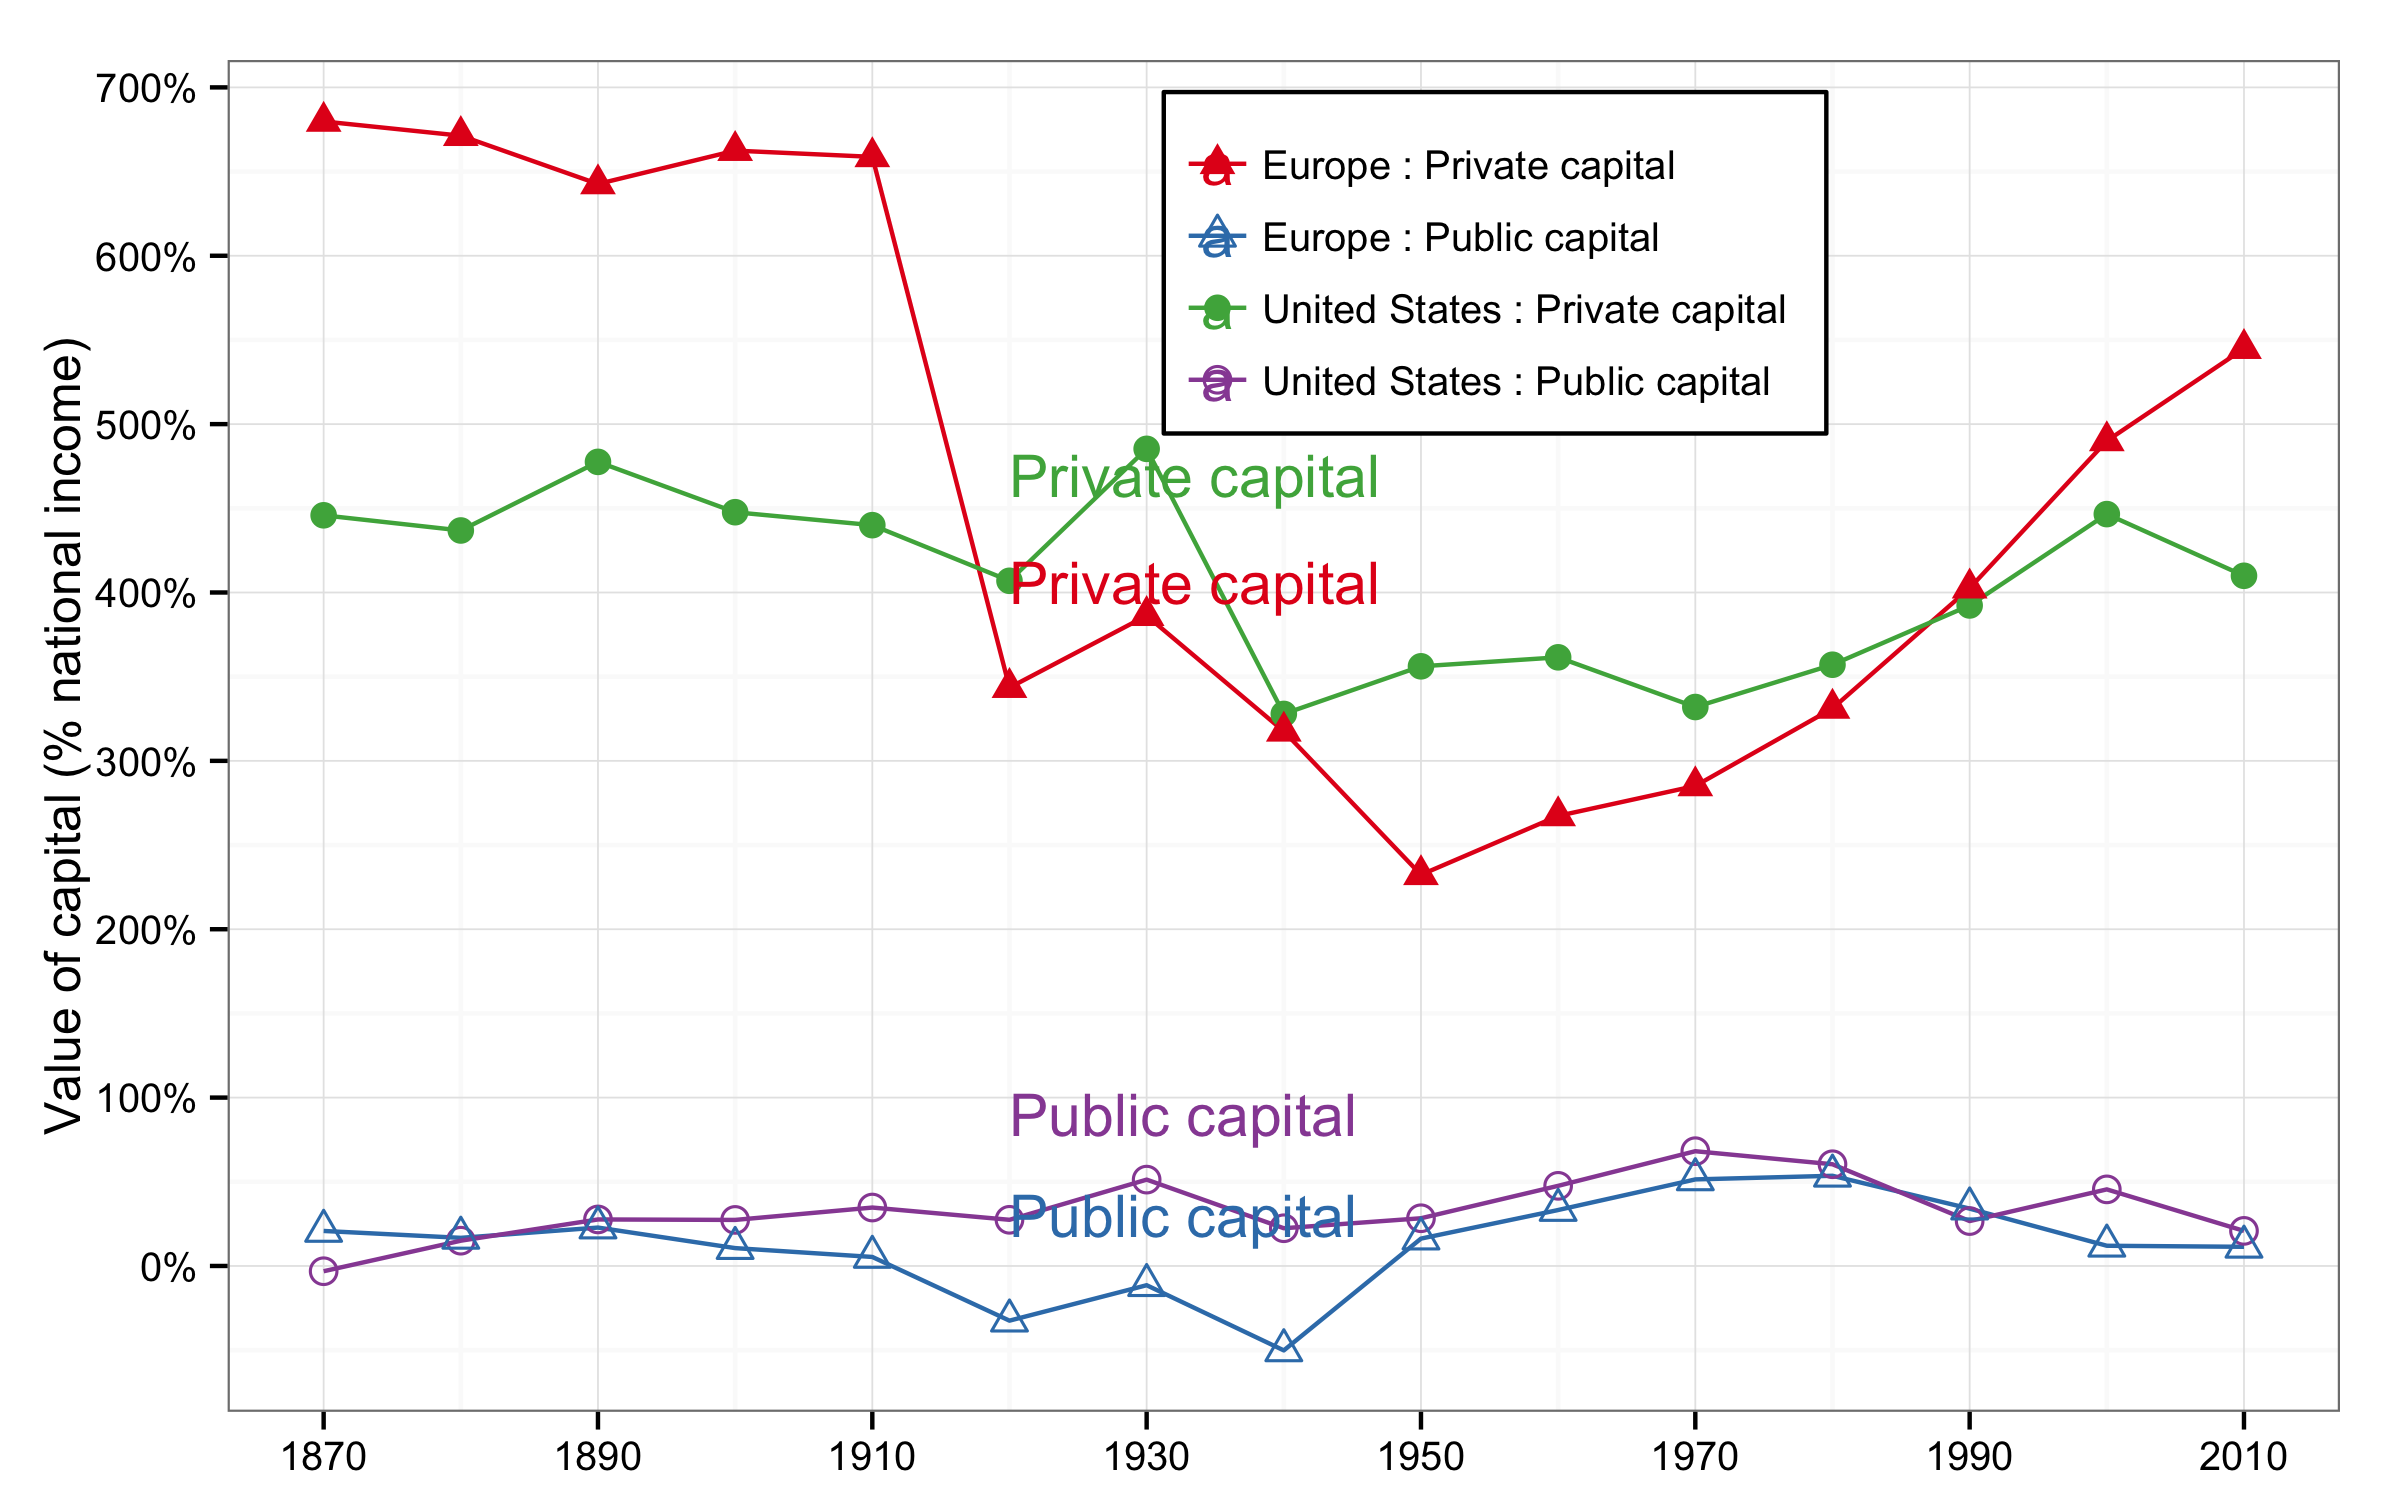
\includegraphics[width=1\linewidth]{figures/color/Figure_5_1} 

}



\end{knitrout}
\caption{The fluctuations of national capital in the long run correspond mostly to the fluctuations of private capital (both in Europe and in the United States).}
\end{minipage}
\end{figure}
\end{frame}
%%%%%%%%%%%%%%%%%%%% Frame Here %%%%%%%%%%%%%%%%%%%%%%%%%%%%%%%%%%%%%%%%%%%%%%%%


%%%%%%%%%%%%%%%%%%%% Frame Here %%%%%%%%%%%%%%%%%%%%%%%%%%%%%%%%%%%%%%%%%%%%%%%%
\begin{frame}[label=Figure_5_2]
\frametitle{Figure 5.2: National capital in Europe \& United States, 1870--2010}
\begin{figure}[t]
\begin{minipage}[b]{\textwidth}
\centering
\begin{knitrout}\footnotesize
\definecolor{shadecolor}{rgb}{0.969, 0.969, 0.969}\color{fgcolor}

{\centering 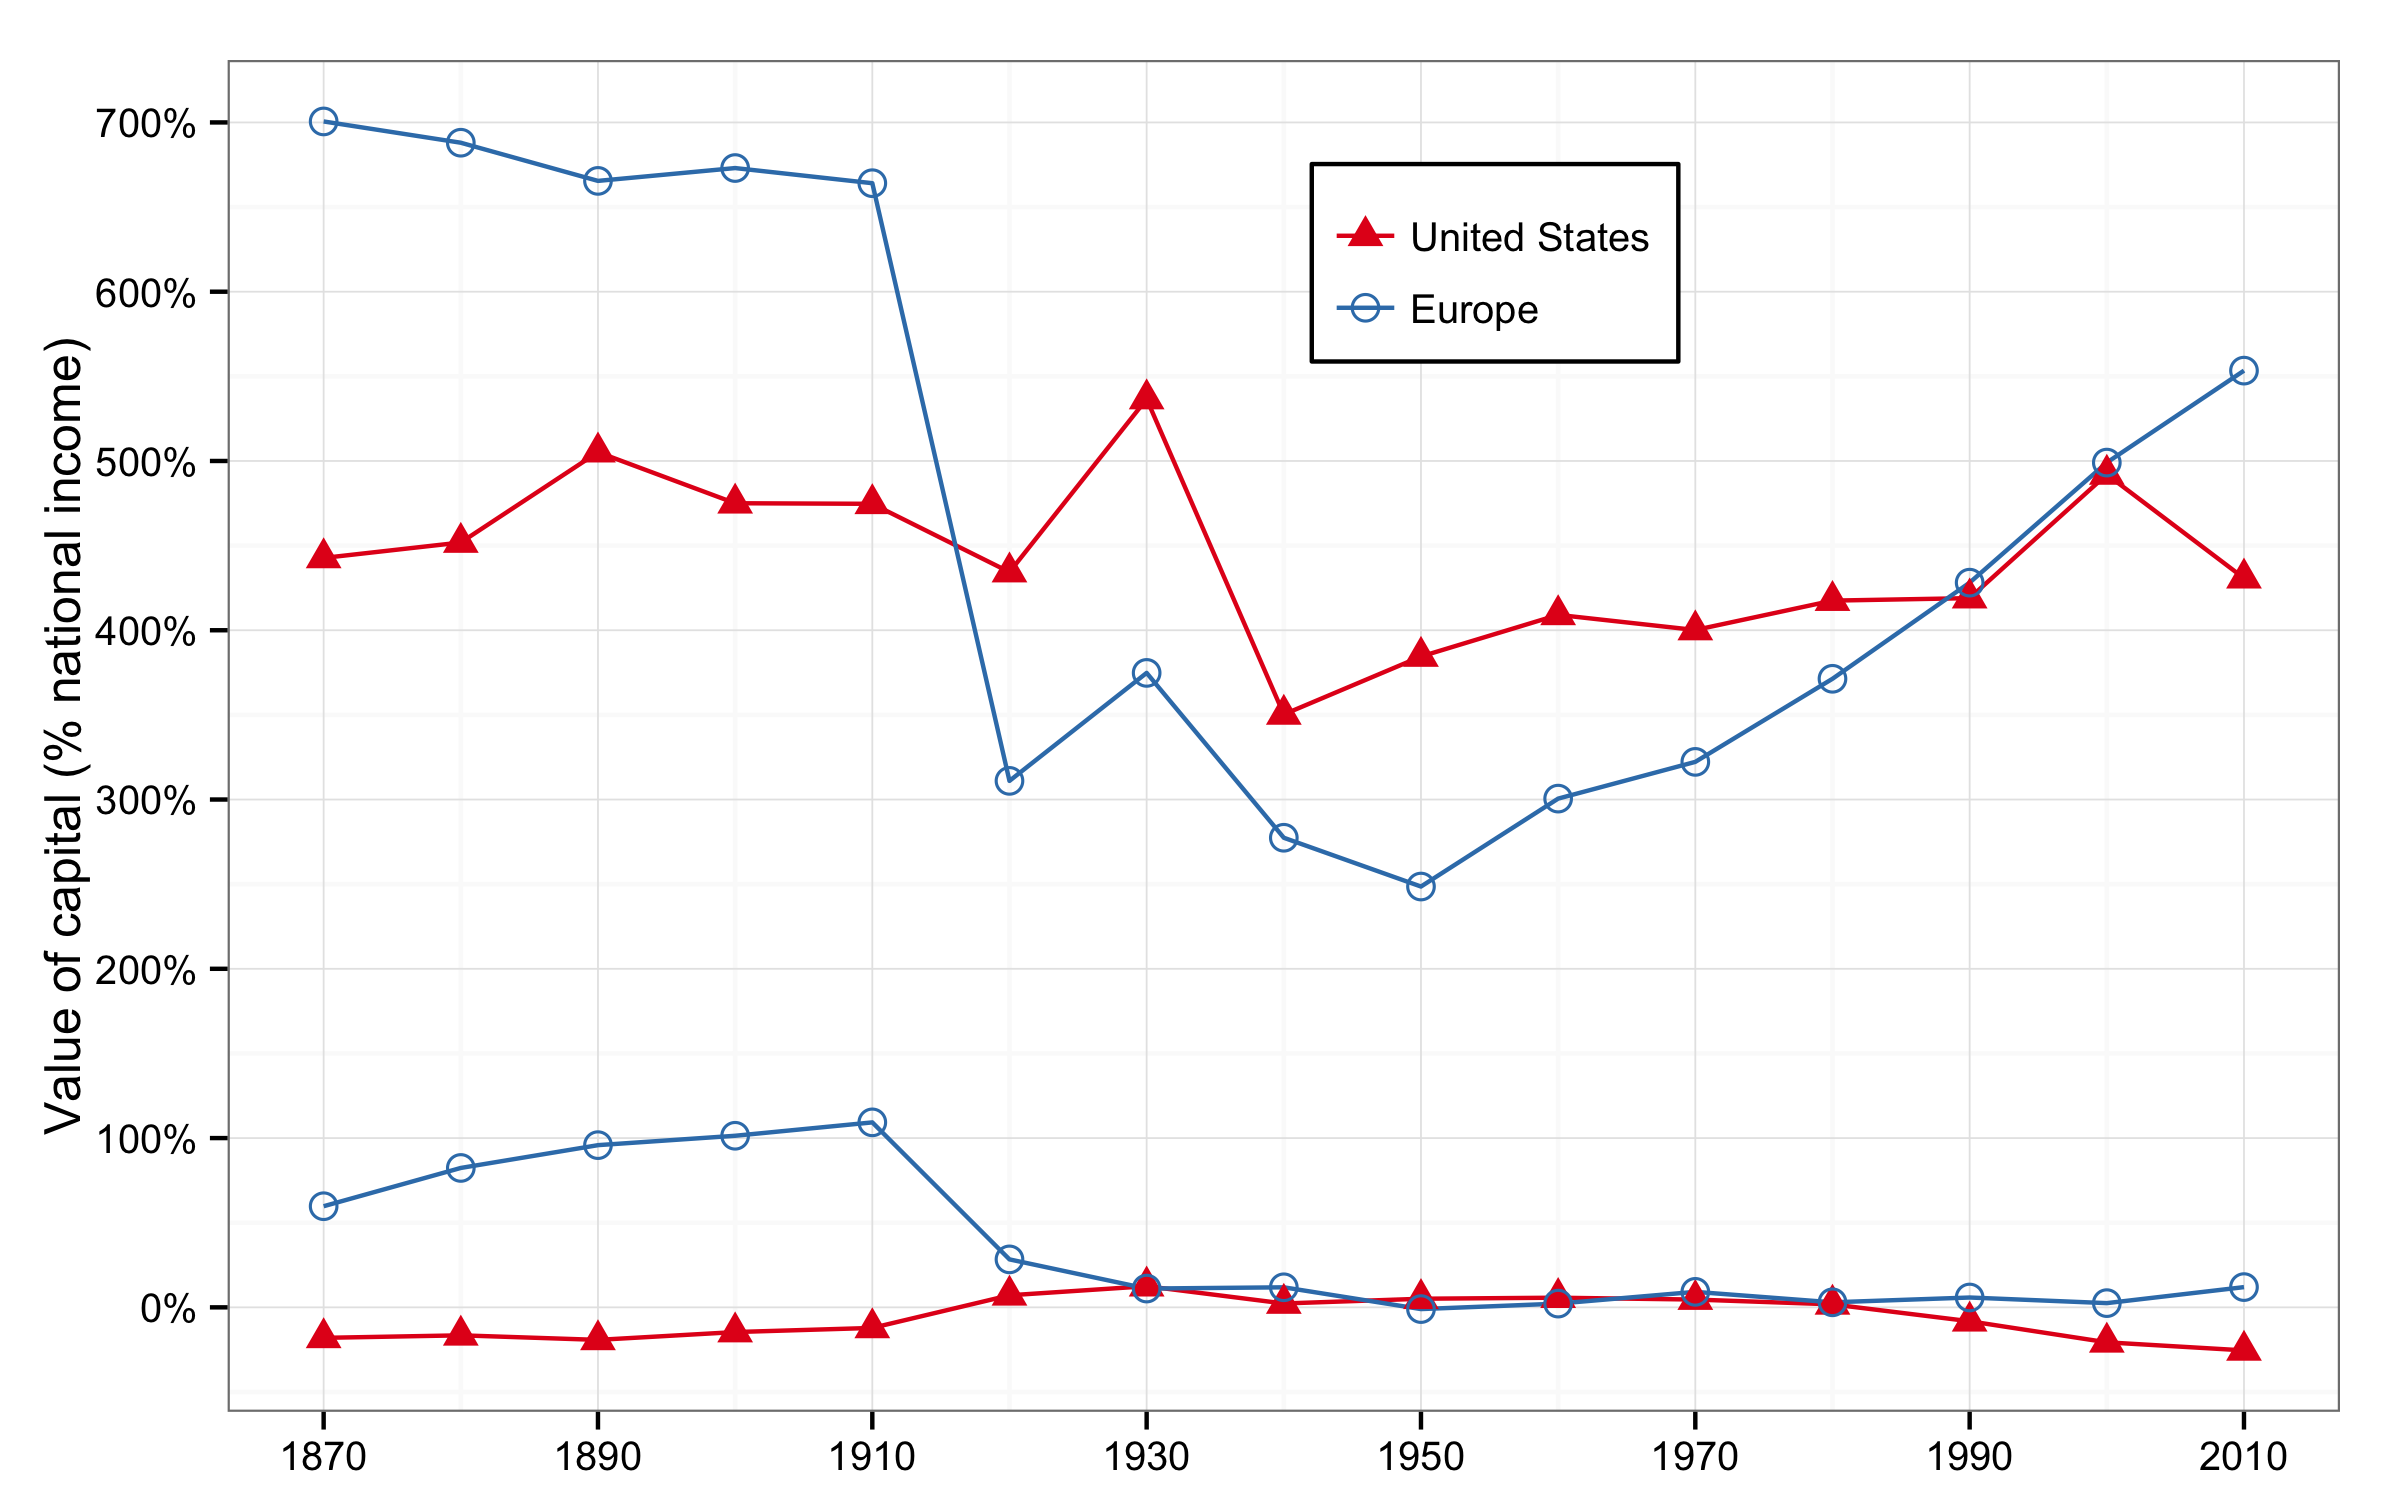
\includegraphics[width=1\linewidth]{figures/color/Figure_5_2} 

}



\end{knitrout}
\caption{National capital (public and private) is worth 6.5 years of national income in Europe in 1910, versus 4.5 years in the United States.}
\end{minipage}
\end{figure}
\end{frame}
%%%%%%%%%%%%%%%%%%%% Frame Here %%%%%%%%%%%%%%%%%%%%%%%%%%%%%%%%%%%%%%%%%%%%%%%%


%%%%%%%%%%%%%%%%%%%% Frame Here %%%%%%%%%%%%%%%%%%%%%%%%%%%%%%%%%%%%%%%%%%%%%%%%
\begin{frame}[label=Figure_5_3]
\frametitle{Figure 5.3: Private capital in rich countries, 1970--2010}
\begin{figure}[t]
\begin{minipage}[b]{\textwidth}
\centering
\begin{knitrout}\footnotesize
\definecolor{shadecolor}{rgb}{0.969, 0.969, 0.969}\color{fgcolor}

{\centering 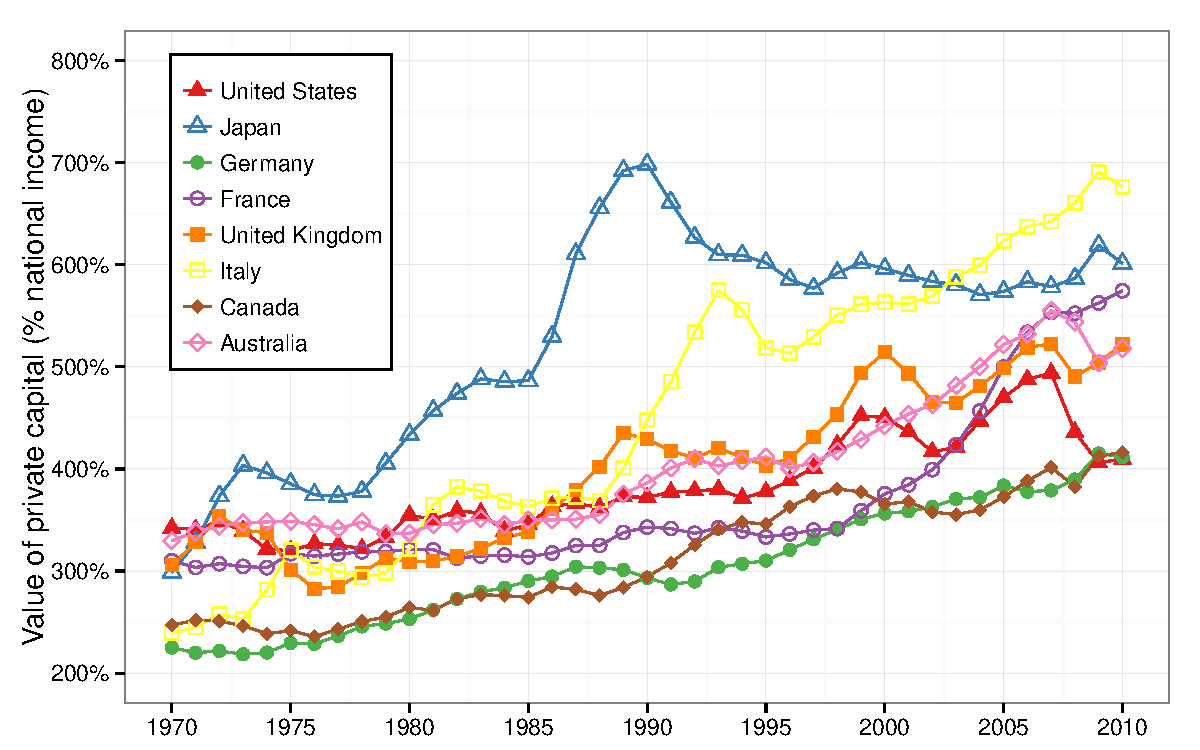
\includegraphics[width=1\linewidth]{figures/color/Figure_5_3} 

}



\end{knitrout}
\caption{Private capital is worth between 2 and 3.5 years of national income in rich countries in 1970, and between 4 and 7 years of national income in 2010.}
\end{minipage}
\end{figure}
\end{frame}
%%%%%%%%%%%%%%%%%%%% Frame Here %%%%%%%%%%%%%%%%%%%%%%%%%%%%%%%%%%%%%%%%%%%%%%%%


%%%%%%%%%%%%%%%%%%%% Frame Here %%%%%%%%%%%%%%%%%%%%%%%%%%%%%%%%%%%%%%%%%%%%%%%%
\begin{frame}[label=Figure_5_3b]
\frametitle{Figure 5.3b: Public capital in rich countries, 1970--2010}
\begin{figure}[t]
\begin{minipage}[b]{\textwidth}
\centering
\begin{knitrout}\footnotesize
\definecolor{shadecolor}{rgb}{0.969, 0.969, 0.969}\color{fgcolor}

{\centering 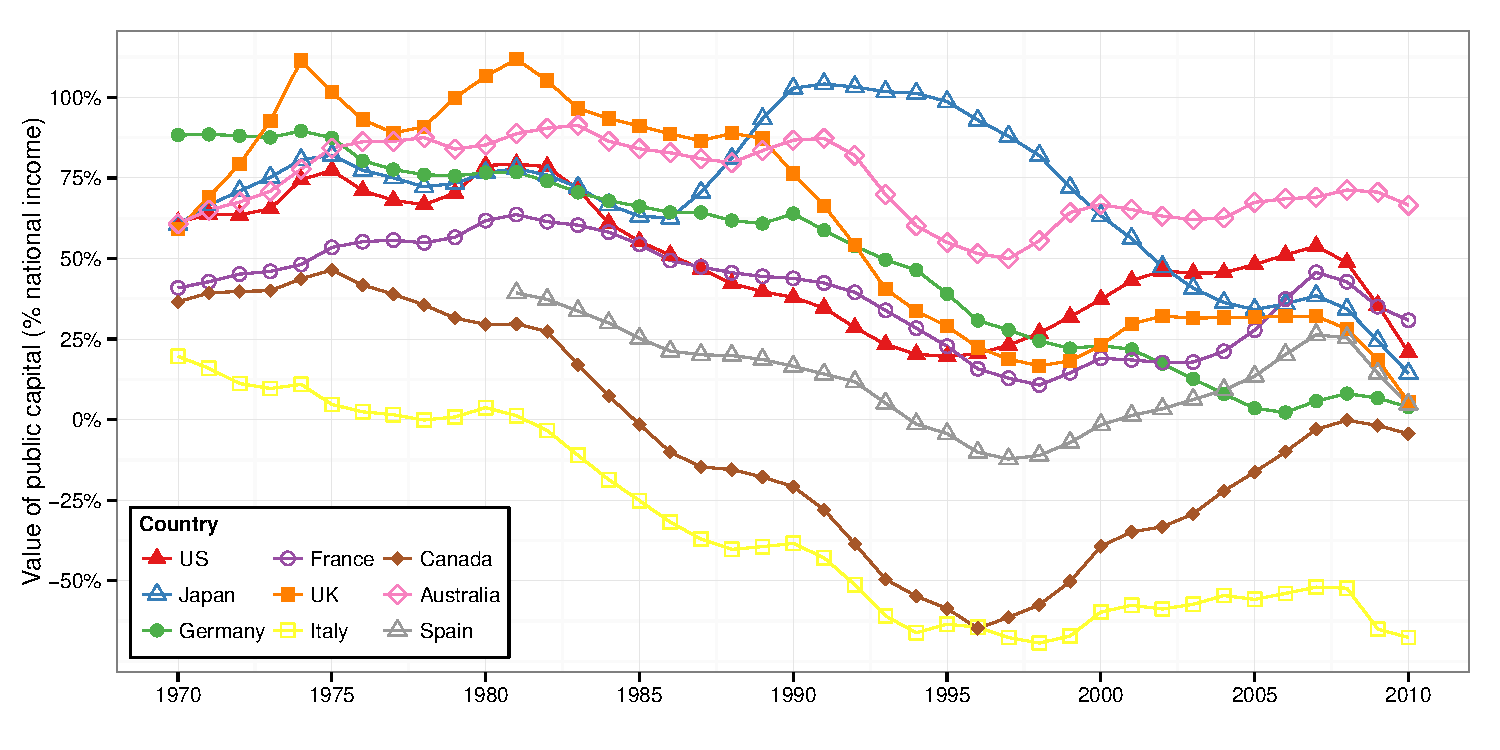
\includegraphics[width=1\linewidth]{figures/color/Figure_5_3b} 

}



\end{knitrout}
\caption{In France, Britain, Germany, and the United States, government deficits exceeded public investment by 2--3\% of national income on average over the period 1970--2010, compared with more than 6\% in Italy.}
\end{minipage}
\end{figure}
\end{frame}
%%%%%%%%%%%%%%%%%%%% Frame Here %%%%%%%%%%%%%%%%%%%%%%%%%%%%%%%%%%%%%%%%%%%%%%%%


%%%%%%%%%%%%%%%%%%%% Frame Here %%%%%%%%%%%%%%%%%%%%%%%%%%%%%%%%%%%%%%%%%%%%%%%%
\begin{frame}[label=Figure_5_4]
\frametitle{Figure 5.4: Private capital in rich countries (ratio), 1970--2010}
\begin{figure}[t]
\begin{minipage}[b]{\textwidth}
\centering
\begin{knitrout}\footnotesize
\definecolor{shadecolor}{rgb}{0.969, 0.969, 0.969}\color{fgcolor}

{\centering 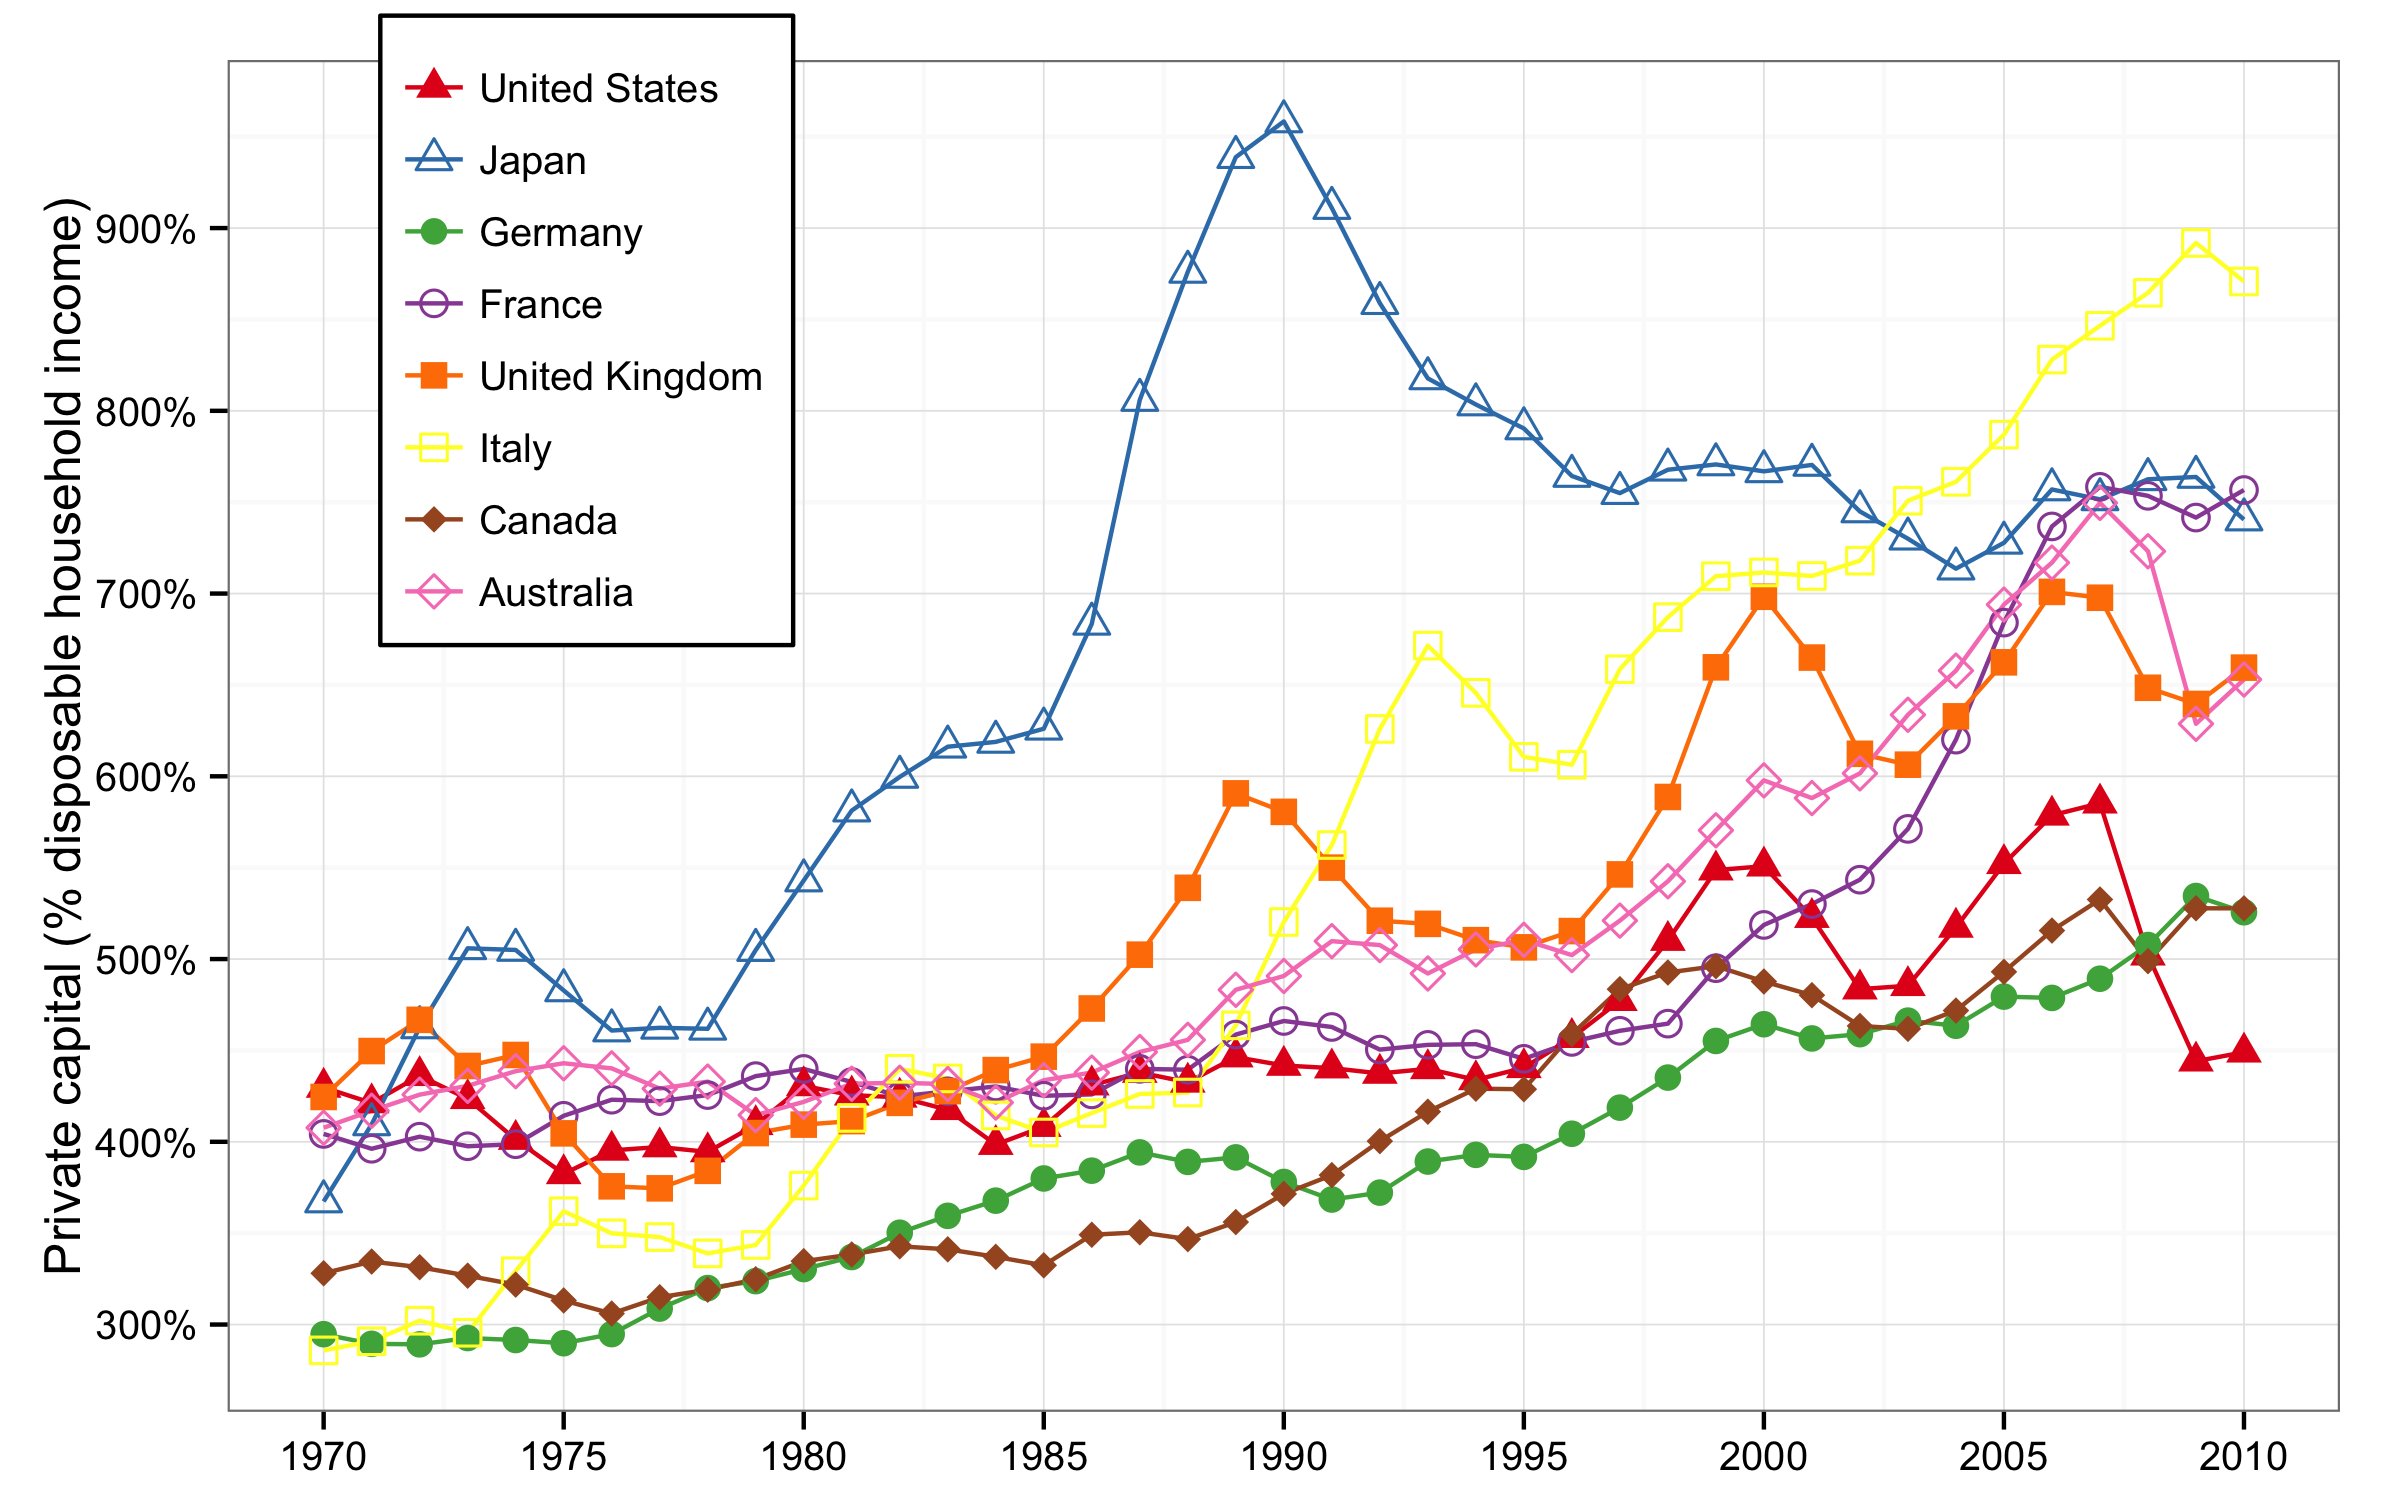
\includegraphics[width=1\linewidth]{figures/color/Figure_5_4} 

}



\end{knitrout}
\caption{Expressed in years of household disposable income (about 70--80\% of national income), the capital/income ratio appears to be larger than when it is expressed in years of national income.}
\end{minipage}
\end{figure}
\end{frame}
%%%%%%%%%%%%%%%%%%%% Frame Here %%%%%%%%%%%%%%%%%%%%%%%%%%%%%%%%%%%%%%%%%%%%%%%%


%%%%%%%%%%%%%%%%%%%% Frame Here %%%%%%%%%%%%%%%%%%%%%%%%%%%%%%%%%%%%%%%%%%%%%%%%
\begin{frame}[label=Figure_5_5]
\frametitle{Figure 5.5: Private and public capital in rich countries, 1970--2010}
\begin{figure}[t]
\begin{minipage}[b]{\textwidth}
\centering
\begin{knitrout}\footnotesize
\definecolor{shadecolor}{rgb}{0.969, 0.969, 0.969}\color{fgcolor}

{\centering 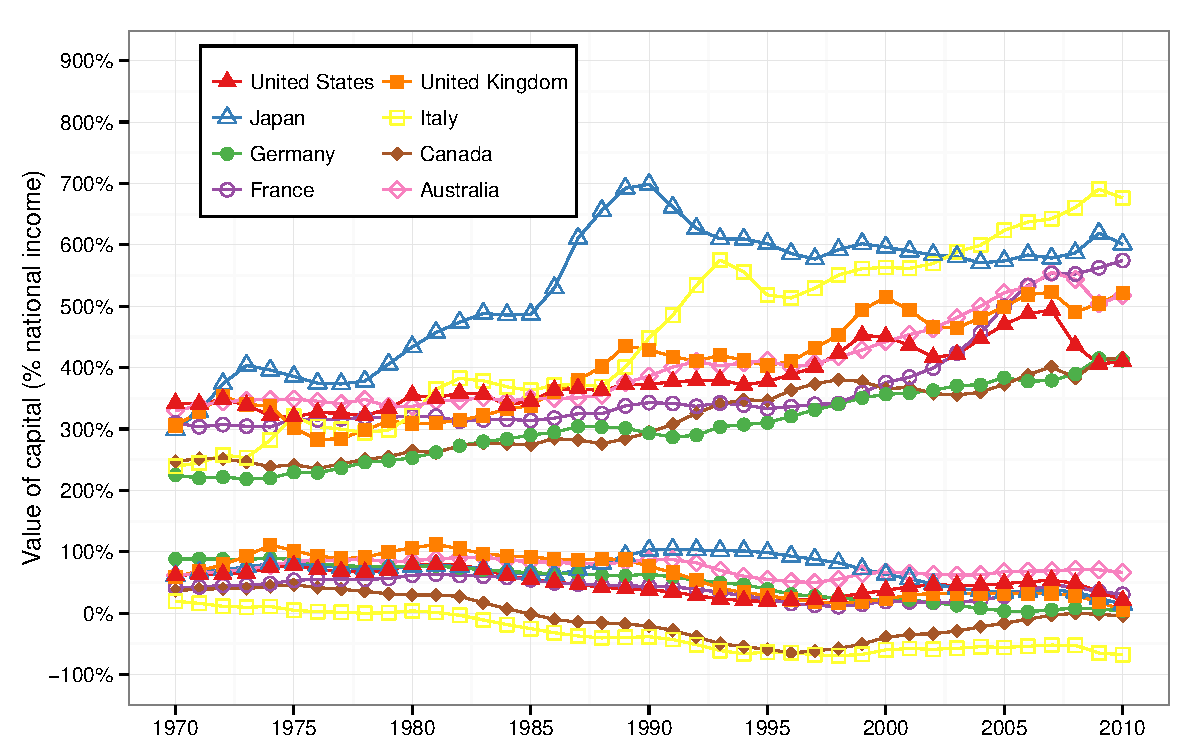
\includegraphics[width=1\linewidth]{figures/color/Figure_5_5} 

}



\end{knitrout}
\caption{In Italy, private capital rose from 240\% to 680\% in national income between 1970 and 2010, while public capital dropped from 20\% to -70\%.}
\end{minipage}
\end{figure}
\end{frame}
%%%%%%%%%%%%%%%%%%%% Frame Here %%%%%%%%%%%%%%%%%%%%%%%%%%%%%%%%%%%%%%%%%%%%%%%%


%%%%%%%%%%%%%%%%%%%% Frame Here %%%%%%%%%%%%%%%%%%%%%%%%%%%%%%%%%%%%%%%%%%%%%%%%
\begin{frame}[label=Figure_5_6]
\frametitle{Figure 5.6: Market value and book value of corporations, 1970--2010}
\begin{figure}[t]
\begin{minipage}[b]{\textwidth}
\centering
\begin{knitrout}\footnotesize
\definecolor{shadecolor}{rgb}{0.969, 0.969, 0.969}\color{fgcolor}

{\centering 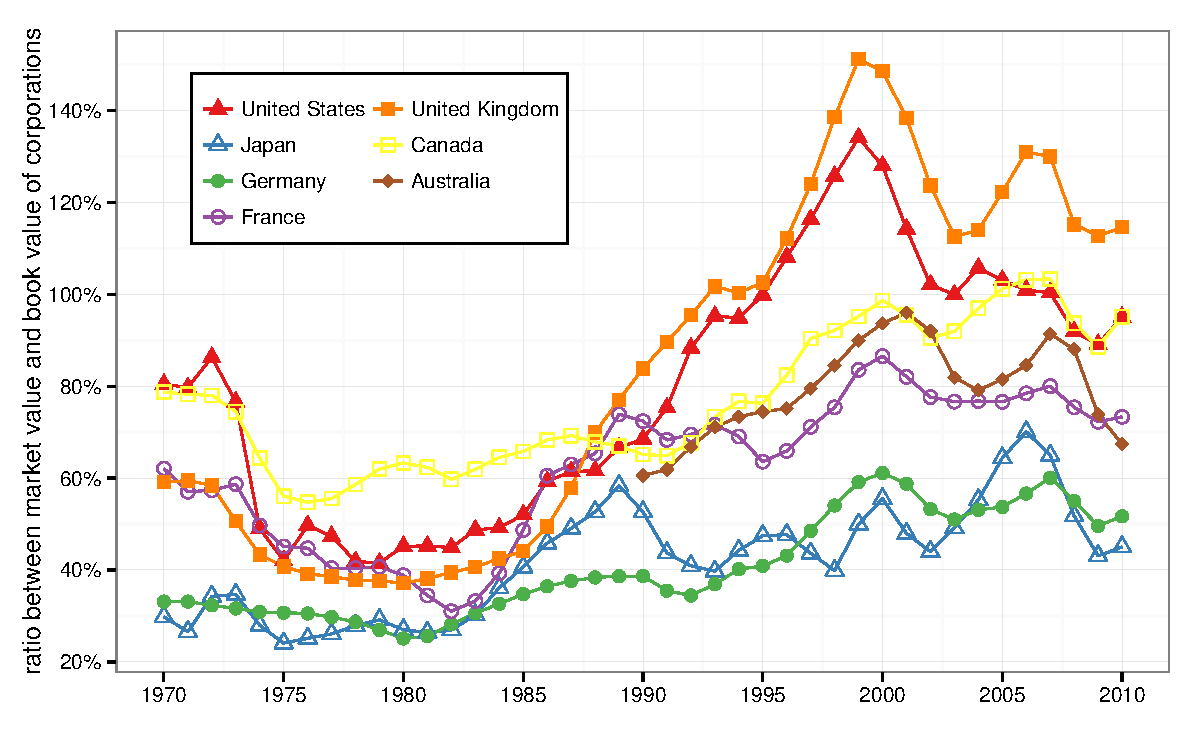
\includegraphics[width=1\linewidth]{figures/color/Figure_5_6} 

}



\end{knitrout}
\caption{Tobin's Q (i.e. the ratio between market value and book value of corporations) has risen in rich countries since the 1970s--1980s.}
\end{minipage}
\end{figure}
\end{frame}
%%%%%%%%%%%%%%%%%%%% Frame Here %%%%%%%%%%%%%%%%%%%%%%%%%%%%%%%%%%%%%%%%%%%%%%%%


%%%%%%%%%%%%%%%%%%%% Frame Here %%%%%%%%%%%%%%%%%%%%%%%%%%%%%%%%%%%%%%%%%%%%%%%%
\begin{frame}[label=Figure_5_7]
\frametitle{Figure 5.7: National capital in rich countries, 1970--2010}
\begin{figure}[t]
\begin{minipage}[b]{\textwidth}
\centering
\begin{knitrout}\footnotesize
\definecolor{shadecolor}{rgb}{0.969, 0.969, 0.969}\color{fgcolor}

{\centering 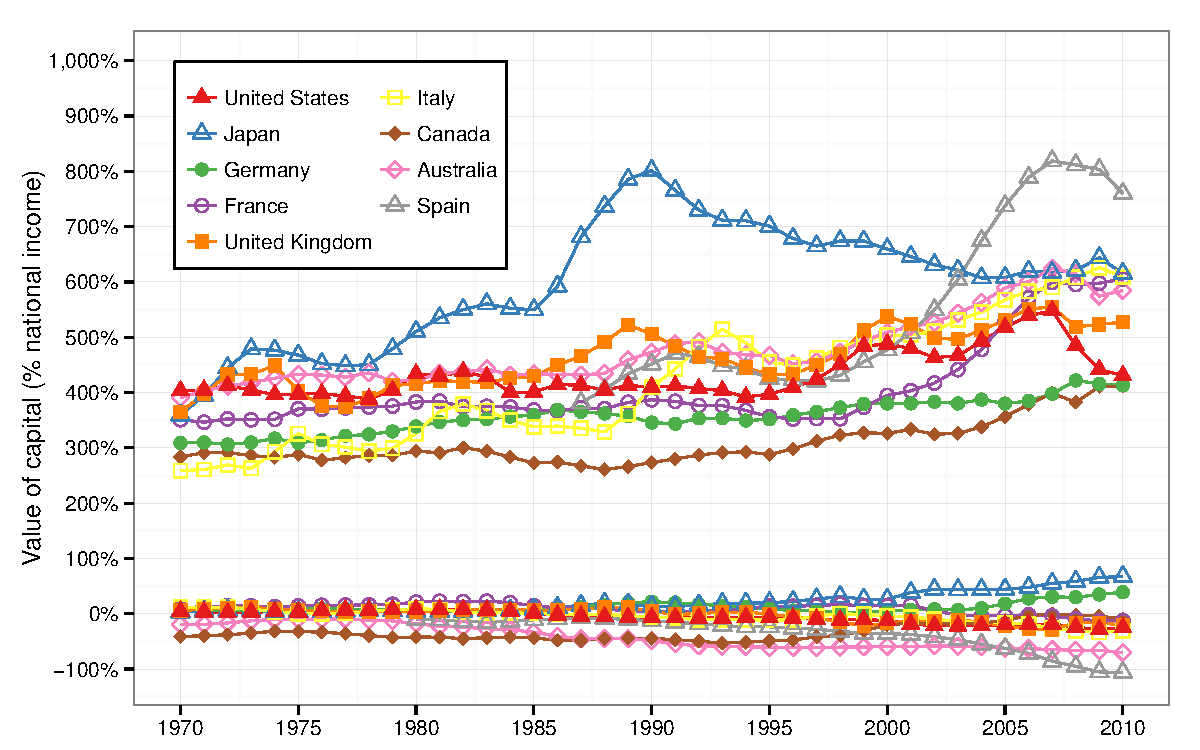
\includegraphics[width=1\linewidth]{figures/color/Figure_5_7} 

}



\end{knitrout}
\caption{Net foreign assets held by Japan and Germany are worth between 6 months and one year of national income in 2010.}
\end{minipage}
\end{figure}
\end{frame}
%%%%%%%%%%%%%%%%%%%% Frame Here %%%%%%%%%%%%%%%%%%%%%%%%%%%%%%%%%%%%%%%%%%%%%%%%


%%%%%%%%%%%%%%%%%%%% Frame Here %%%%%%%%%%%%%%%%%%%%%%%%%%%%%%%%%%%%%%%%%%%%%%%%
\begin{frame}[label=Figure_5_8]
\frametitle{Figure 5.8: The world capital/income ratio, 1870--2100}
\begin{figure}[t]
\begin{minipage}[b]{\textwidth}
\centering
\begin{knitrout}\footnotesize
\definecolor{shadecolor}{rgb}{0.969, 0.969, 0.969}\color{fgcolor}

{\centering 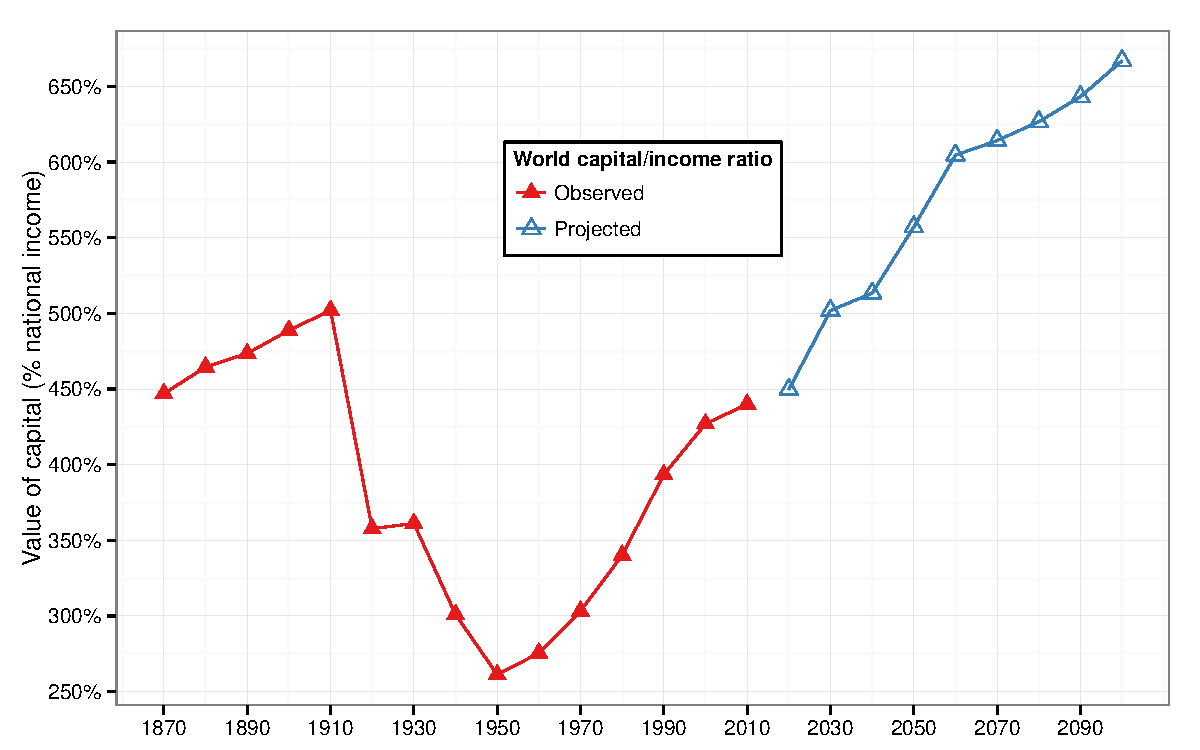
\includegraphics[width=1\linewidth]{figures/color/Figure_5_8} 

}



\end{knitrout}
\caption{According to simulations (central scenario), the world capital/income ratio could be close to 700 percent by the end of the twenty-first century.}
\end{minipage}
\end{figure}
\end{frame}
%%%%%%%%%%%%%%%%%%%% Frame Here %%%%%%%%%%%%%%%%%%%%%%%%%%%%%%%%%%%%%%%%%%%%%%%%


%%%%%%%%%%%%%%%%%%%% Frame Here %%%%%%%%%%%%%%%%%%%%%%%%%%%%%%%%%%%%%%%%%%%%%%%%
\begin{frame}[label=Table_12_1]
\frametitle{Table 12.1: The growth rate of top global wealth, 1987--2013}
\begin{table}[t]
%\caption{The growth rate of top global wealth, 1987--2013}
\adjustbox{max height=\dimexpr\textheight-5.5cm\relax,
           max width=\textwidth}{%
\begin{threeparttable}
\centering
\begin{tabular}{@{}lc@{}}
\toprule
    & Average real growth rate per year  \\
    & (after deduction of inflation) (\%) \\
\midrule
    The top 1/(100 million) highest wealth holders \tnote{a}   & 6.8  \\
    The top 1/(20 million)  highest wealth holders \tnote{b}   & 6.4  \\
    Average world wealth per adult                             & 2.1  \\
    Average world income per adult                             & 1.4  \\
    World adult population                                     & 1.9  \\
    World GDP                                                  & 3.3  \\
\midrule
\end{tabular}
\begin{tablenotes}
    \item Between 1987 and 2013, the highest global wealth fractiles have grown at 6--7\% per year versus 2.1\% for average world wealth, and 1.4\% for average world income. All growth rates are net of inflation (2.3\% per year between 1987 and 2013).
    \item[a] About 30 adults out of 3 billion in the 1980s, and 45 adults out of 4.5 billion in 2010.
    \item[b] About 150 adults out of 3 billion in the 1980s, and 225 adults out of 4.5 billion in the 2010s.
\end{tablenotes}
\end{threeparttable}}
\end{table}
\end{frame}
%%%%%%%%%%%%%%%%%%%% Frame Here %%%%%%%%%%%%%%%%%%%%%%%%%%%%%%%%%%%%%%%%%%%%%%%%


%%%%%%%%%%%%%%%%%%%% Frame Here %%%%%%%%%%%%%%%%%%%%%%%%%%%%%%%%%%%%%%%%%%%%%%%%
\begin{frame}[label=Table_12_2]
\frametitle{Table 12.2: The return on the capital endowments of U.S. universities, 1980--2010}
\begin{table}[t]
%\caption{The return on the capital endowments of U.S. universities, 1980--2010}
\adjustbox{max height=\dimexpr\textheight-5.5cm\relax,
           max width=\textwidth}{%
\begin{threeparttable}
\centering
\begin{tabular}{@{}lc@{}}
\toprule
    & Average real annual rate of return                           \\
    & (after deduction of inflation and all                        \\
    & administrative costs and financial fees) (\%)                \\
\midrule
    All universities (850)                                & 8.2    \\
    Harvard, Yale, and Princeton                          & 10.2   \\
    Endowments higher than \$1 billion (60)               & 8.8    \\
    Endowments between \$500 million and 1 billion (66)   & 7.8    \\
    Endowments between \$100 and \$500 million (226)      & 7.1    \\
    Endowments less than \$100 million (498)              & 6.2    \\
\midrule
\end{tabular}
\begin{tablenotes}
    \item Between 1980 and 2010, U.S. universities earned an average real rate of return of 8.2\% on their capital endowments, and more for the greater endowments. All returns are reported net of inflation (2.4\% per year between 1980 and 2010) and net of administrative costs and financial fees.
\end{tablenotes}
\end{threeparttable}}
\end{table}
\end{frame}
%%%%%%%%%%%%%%%%%%%% Frame Here %%%%%%%%%%%%%%%%%%%%%%%%%%%%%%%%%%%%%%%%%%%%%%%%


%%%%%%%%%%%%%%%%%%%% Frame Here %%%%%%%%%%%%%%%%%%%%%%%%%%%%%%%%%%%%%%%%%%%%%%%%
\begin{frame}[label=Figure_9_8]
\frametitle{Figure 9.8: Income inequality: Europe vs. United States, 1900--2010}
\begin{figure}[t]
\begin{minipage}[b]{\textwidth}
\centering
\begin{knitrout}\footnotesize
\definecolor{shadecolor}{rgb}{0.969, 0.969, 0.969}\color{fgcolor}

{\centering 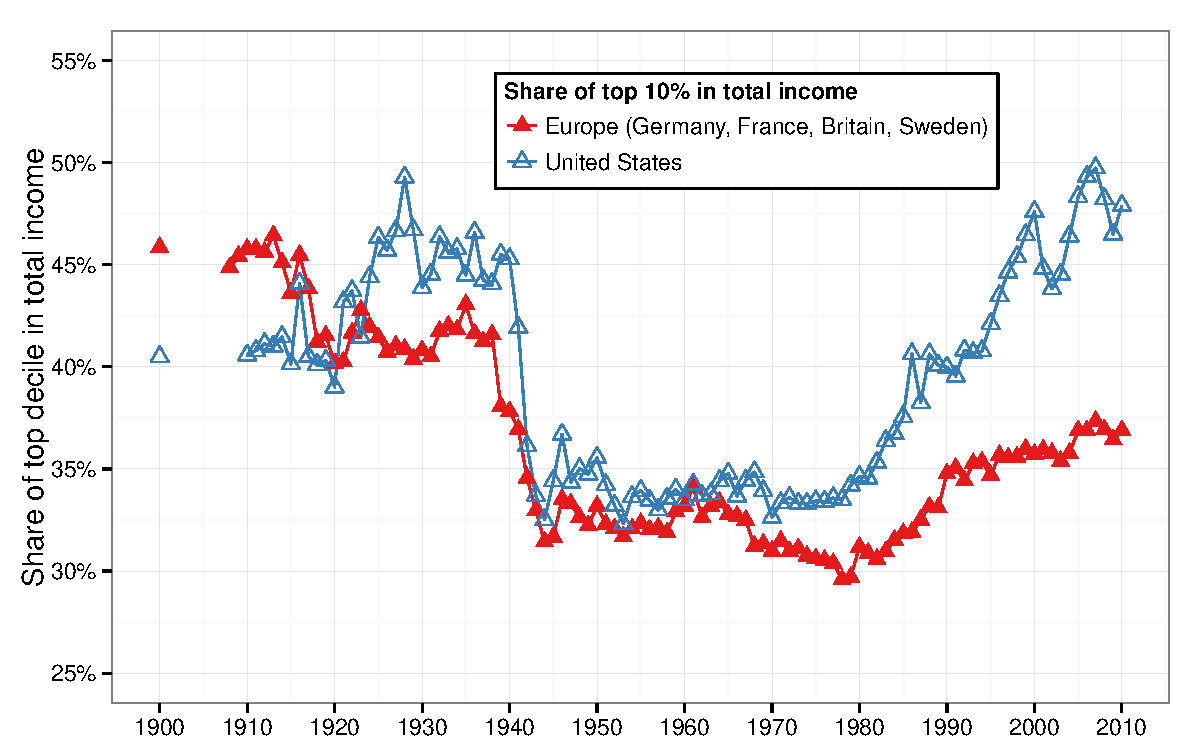
\includegraphics[width=1\linewidth]{figures/color/Figure_9_8} 

}



\end{knitrout}
\caption{The top decile income share was higher in Europe than in the U.S. in 1900--2010. It is much higher in the U.S. in 2000--2010.}
\end{minipage}
\end{figure}
\end{frame}
%%%%%%%%%%%%%%%%%%%% Frame Here %%%%%%%%%%%%%%%%%%%%%%%%%%%%%%%%%%%%%%%%%%%%%%%%


%%%%%%%%%%%%%%%%%%%% Frame Here %%%%%%%%%%%%%%%%%%%%%%%%%%%%%%%%%%%%%%%%%%%%%%%%
\begin{frame}[label=Figure_14_1]
\frametitle{Figure 14.1: Top income tax rates, 1900--2013}
\begin{figure}[t]
\begin{minipage}[b]{\textwidth}
\centering
\begin{knitrout}\footnotesize
\definecolor{shadecolor}{rgb}{0.969, 0.969, 0.969}\color{fgcolor}

{\centering 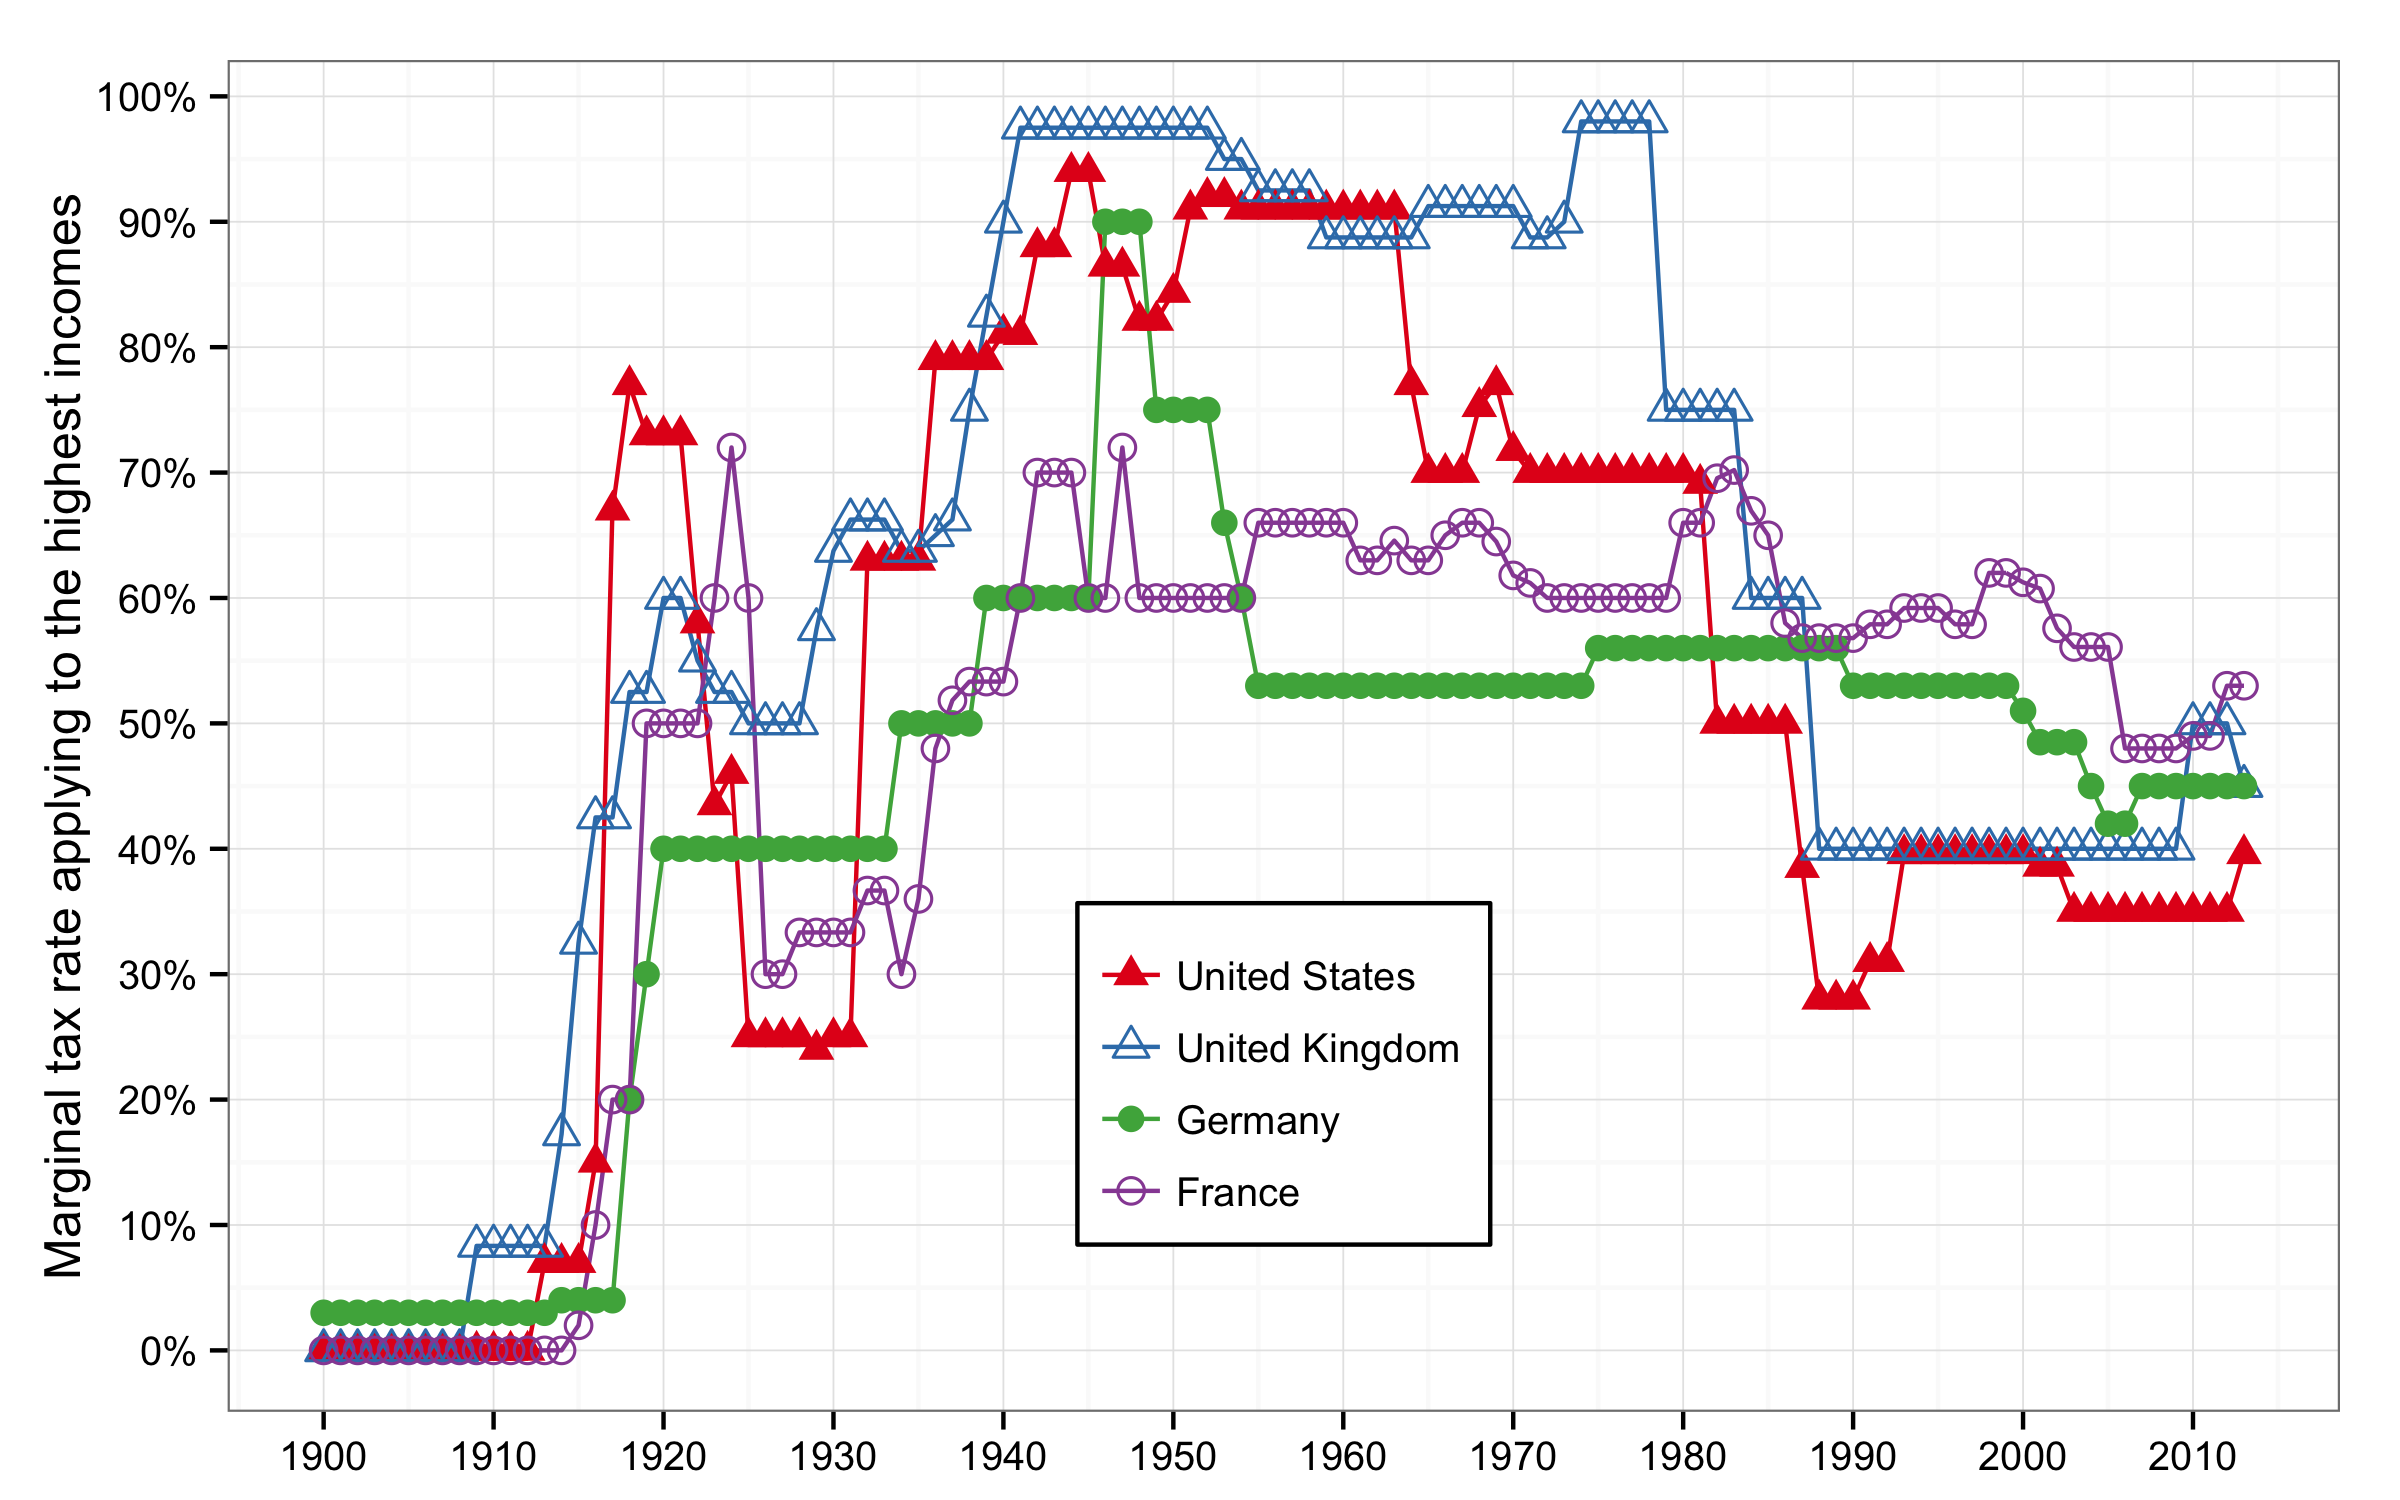
\includegraphics[width=1\linewidth]{figures/color/Figure_14_1} 

}



\end{knitrout}
\caption{The top marginal tax rate of the income tax (applying to the highest incomes) in the U.S. dropped from 70\% in 1980 to 28\% in 1988.}
\end{minipage}
\end{figure}
\end{frame}
%%%%%%%%%%%%%%%%%%%% Frame Here %%%%%%%%%%%%%%%%%%%%%%%%%%%%%%%%%%%%%%%%%%%%%%%%


%%%%%%%%%%%%%%%%%%%% Frame Here %%%%%%%%%%%%%%%%%%%%%%%%%%%%%%%%%%%%%%%%%%%%%%%%
\begin{frame}[label=Figure_14_2]
\frametitle{Figure 14.2: Top inheritance tax rates, 1900--2013}
\begin{figure}[t]
\begin{minipage}[b]{\textwidth}
\centering
\begin{knitrout}\footnotesize
\definecolor{shadecolor}{rgb}{0.969, 0.969, 0.969}\color{fgcolor}

{\centering 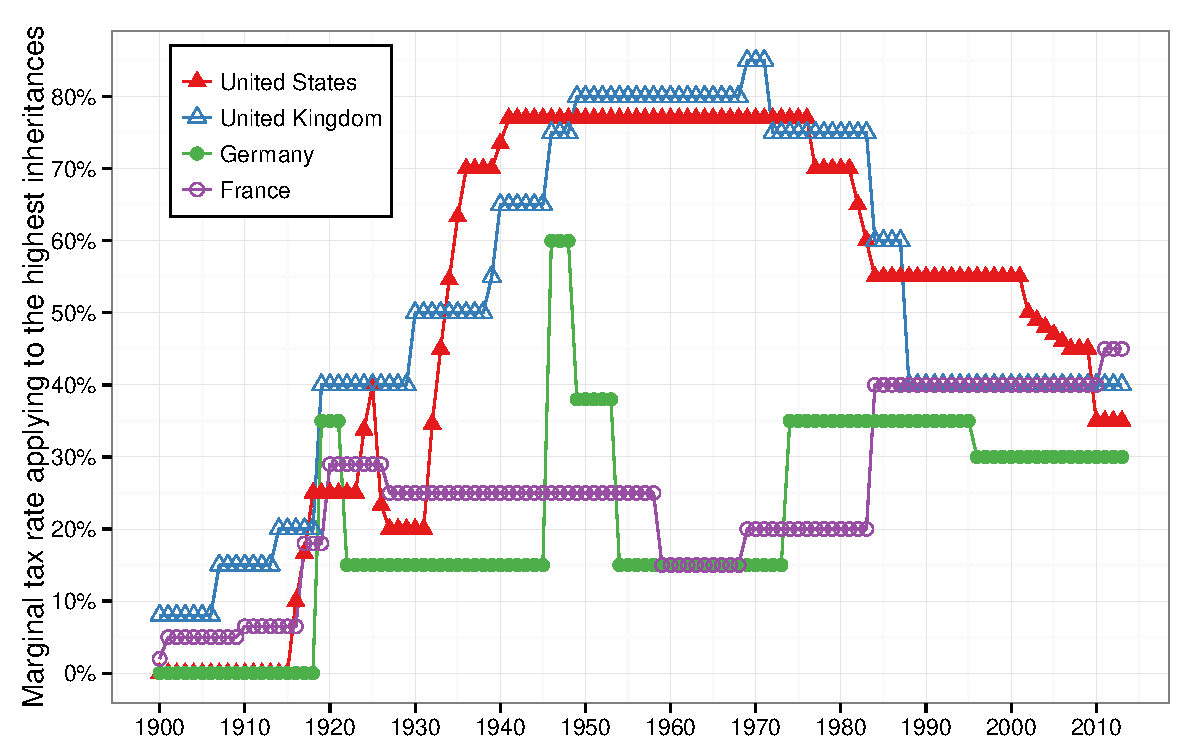
\includegraphics[width=1\linewidth]{figures/color/Figure_14_2} 

}



\end{knitrout}
\caption{The top marginal tax rate of the inheritance tax (applying to the highest inheritances) in the U.S. dropped from 70\% in 1980 to 35\% in 2013.}
\end{minipage}
\end{figure}
\end{frame}
%%%%%%%%%%%%%%%%%%%% Frame Here %%%%%%%%%%%%%%%%%%%%%%%%%%%%%%%%%%%%%%%%%%%%%%%%


%%%%%%%%%%%%%%%%%%%% Frame Here %%%%%%%%%%%%%%%%%%%%%%%%%%%%%%%%%%%%%%%%%%%%%%%%
\begin{frame}[label=Conclusions_1,shrink=7]
\frametitle{Conclusions}
\begin{itemize}
\item
\textbf{The history of income and wealth inequality is always political, chaotic and unpredictable; it involves national identities and sharp reversals; nobody can predict the reversals of the future.}
\item
Marx: with $g=0$, $\beta \to \infty$, $r \to 0$ : revolution, war
\item
My conclusions are less apocalyptic: with $g>0$, at least we have a steady state $\beta = s/g$.
\item
But with $g>0$ \& small, this steady-state can be rather gloomy: it can involve a very large capital-income ratio $\beta$ and capital share $\alpha$, as well as extreme wealth concentration due to high $r-g$.
\item
This has nothing to do with a market imperfection: the more perfect the capital market, the higher $r-g$.
\item
The ideal solution: progressive wealth tax at the global scale, based upon automatic exchange of bank information.
\item
Other solutions involve authoritarian political \& capital controls (China, Russia..), or perpetual population growth (US), or inflation, or some mixture of all.
\end{itemize}
\end{frame}
%%%%%%%%%%%%%%%%%%%% Frame Here %%%%%%%%%%%%%%%%%%%%%%%%%%%%%%%%%%%%%%%%%%%%%%%%


%%%%%%%%%%%%%%%%%%%% Frame Here %%%%%%%%%%%%%%%%%%%%%%%%%%%%%%%%%%%%%%%%%%%%%%%%
\begin{frame}[label=Transition_1]
\begin{center}
\begin{huge}
Supplementary Slides
\vspace{3\baselineskip}\par
(long lecture version)
\end{huge}
\end{center}
\end{frame}
%%%%%%%%%%%%%%%%%%%% Frame Here %%%%%%%%%%%%%%%%%%%%%%%%%%%%%%%%%%%%%%%%%%%%%%%%


% Long Version Starts Here


%%%%%%%%%%%%%%%%%%%% Frame Here %%%%%%%%%%%%%%%%%%%%%%%%%%%%%%%%%%%%%%%%%%%%%%%%
\begin{frame}[label=WealthReturn,shrink=8]
\frametitle{1. The return of a wealth-based society}
\begin{itemize}
\item
Wealth = capital $K$ = everything we own and that can be sold on a market (net of all debts) (excludes human $K$, except in slave societies)
\item
In textbooks, wealth-income \& capital-ouput ratios are supposed to be constant. But the so-called ``Kaldor facts'' actually rely on little historical evidence.
\item
In fact, we observe in Europe \& Japan a large recovery of $\beta=K/Y$ in recent decades:
\begin{align*}
\beta = 200-300\% ~\text{in}~ 1950-1960 \\
\beta = 500-600\% ~\text{in}~ 2000-2010
\end{align*}
\begin{footnotesize}
(i.e. average wealth $K$ was about 2--3 years of average income $Y$ around 1950--1960; it is about 5--6 years in 2000--2010)
\linebreak
(with $\beta \simeq 600\%$, if $Y \simeq \euro 30,000$ per capita, then $K \simeq \euro 180,000$ per capita) (currently, $K \simeq$ half real estate, half financial assets)
\end{footnotesize}
\item
\textbf{Are we heading back to the $\beta = 600-700\%$ observed in the wealth-based societies of 18c-19c? Or even more?}
\end{itemize}
\end{frame}
%%%%%%%%%%%%%%%%%%%% Frame Here %%%%%%%%%%%%%%%%%%%%%%%%%%%%%%%%%%%%%%%%%%%%%%%%


\againframe{Figure_5_3}


\againframe{Figure_5_5}


\againframe{Figure_5_7}


%%%%%%%%%%%%%%%%%%%% Frame Here %%%%%%%%%%%%%%%%%%%%%%%%%%%%%%%%%%%%%%%%%%%%%%%%
\begin{frame}[label=Figure_3_1]
\frametitle{Figure 3.1: Capital in Britain, 1700--2010}
\begin{figure}[t]
\begin{minipage}[b]{\textwidth}
\centering

\caption{National capital is worth about seven years of national income in Britain in 1700 (including four in agricultural land).}
\end{minipage}
\end{figure}
\end{frame}
%%%%%%%%%%%%%%%%%%%% Frame Here %%%%%%%%%%%%%%%%%%%%%%%%%%%%%%%%%%%%%%%%%%%%%%%%


%%%%%%%%%%%%%%%%%%%% Frame Here %%%%%%%%%%%%%%%%%%%%%%%%%%%%%%%%%%%%%%%%%%%%%%%%
\begin{frame}[label=Figure_3_2]
\frametitle{Figure 3.2: Capital in France, 1700--2010}
\begin{figure}[t]
\begin{minipage}[b]{\textwidth}
\centering

\caption{National capital is worth almost seven years of national income in France in 1910 (including one invested abroad).}
\end{minipage}
\end{figure}
\end{frame}
%%%%%%%%%%%%%%%%%%%% Frame Here %%%%%%%%%%%%%%%%%%%%%%%%%%%%%%%%%%%%%%%%%%%%%%%%



%%%%%%%%%%%%%%%%%%%% Frame Here %%%%%%%%%%%%%%%%%%%%%%%%%%%%%%%%%%%%%%%%%%%%%%%%
\begin{frame}[label=CapitalIsBack]
\frametitle{Capital is back}
\begin{itemize}
\item
The simplest way to think about this is the following: 
\begin{itemize}
\item
In the long-run, $\beta = s/g$
\par\medskip
with $s$ = (net-of-depreciation) saving rate and $g$ = economy's growth rate (population + productivity).
\end{itemize}
\item
With $s = 10\%$, $g = 3\%$, $\beta \simeq 300\%$; but if $s = 10\%$, $g = 1.5\%$, $\beta \simeq 600\%$.
\item
\textbf{In slow-growth societies, the total stock of wealth accumulated in the past can naturally be very important.}
\item
$\rightarrow$ \textbf{capital is back because low growth is back.}
(in particular because population growth $\downarrow 0$)
\item
$\rightarrow$ \textbf{in the long run, this can be relevant for the entire planet.}
\item
Note: $\beta = s/g$ = pure stock-flow accounting identity; it is true whatever the combination of saving motives.
\end{itemize}
\end{frame}
%%%%%%%%%%%%%%%%%%%% Frame Here %%%%%%%%%%%%%%%%%%%%%%%%%%%%%%%%%%%%%%%%%%%%%%%%


%%%%%%%%%%%%%%%%%%%% Frame Here %%%%%%%%%%%%%%%%%%%%%%%%%%%%%%%%%%%%%%%%%%%%%%%%
\begin{frame}[label=Figure_12_5]
\frametitle{Figure 12.5: }
\begin{figure}[t]
\begin{minipage}[b]{\textwidth}
\centering

\caption{.}
\end{minipage}
\end{figure}
\end{frame}
%%%%%%%%%%%%%%%%%%%% Frame Here %%%%%%%%%%%%%%%%%%%%%%%%%%%%%%%%%%%%%%%%%%%%%%%%


%%%%%%%%%%%%%%%%%%%% Frame Here %%%%%%%%%%%%%%%%%%%%%%%%%%%%%%%%%%%%%%%%%%%%%%%%
\begin{frame}[label=ElasticityKL,shrink=14]
\frametitle{The capital--labor elasticity of substitution}
\begin{itemize}
\item
\textbf{Will the rise of capital income-ratio $\beta$ also lead to a rise of the capital share $\alpha$ in national income?}
\item
If the capital stock equals $\beta = 6$ years of income and the average return to capital is equal $r = 5\%$ per year, then the share of capital income (rent, dividends, interest, profits, etc.) in national income equals $\alpha = r \times \beta = 30\%$.
\item
Technically, whether a rise in $\beta$ also leads to a rise in capital share $\alpha = r \beta$ depends on the elasticity of substitution $\sigma$ between capital $K$ and labor $L$ in the production function $Y = F(K, L)$.
\item
Intuition: $\sigma$ measures the extent to which workers can be replaced by machines (e.g. Amazon’s drones).
\item
Standard assumption: Cobb-Douglas production function ($\sigma = 1$) = as the stock $\beta \uparrow$, the return $r \downarrow$ exactly in the same proportions, so that $\alpha = r \times \beta$ remains unchanged, like by magic = a stable world where the capital--labor split is entirely set by technology.
\item
But if $\sigma > 1$, then the return to capital $r \downarrow$ falls less than the volume of capital $\beta\uparrow$, so that the product $\alpha = r \times \beta \uparrow$.
\item
\textbf{Exactly what happened since the 1970s--80s: both the ratio $\beta$ and the capital share $\alpha$ have increased.}
\end{itemize}
\end{frame}
%%%%%%%%%%%%%%%%%%%% Frame Here %%%%%%%%%%%%%%%%%%%%%%%%%%%%%%%%%%%%%%%%%%%%%%%%


%%%%%%%%%%%%%%%%%%%% Frame Here %%%%%%%%%%%%%%%%%%%%%%%%%%%%%%%%%%%%%%%%%%%%%%%%
\begin{frame}[label=Figure_6_5]
\frametitle{Figure 6.5: }
\begin{figure}[t]
\begin{minipage}[b]{\textwidth}
\centering

\caption{.}
\end{minipage}
\end{figure}
\end{frame}
%%%%%%%%%%%%%%%%%%%% Frame Here %%%%%%%%%%%%%%%%%%%%%%%%%%%%%%%%%%%%%%%%%%%%%%%%


%%%%%%%%%%%%%%%%%%%% Frame Here %%%%%%%%%%%%%%%%%%%%%%%%%%%%%%%%%%%%%%%%%%%%%%%%
\begin{frame}[label=Robots]
\frametitle{Towards a world of robots?}
\begin{itemize}
\item
With a large rise in $\beta$, one can get large rise in $\alpha$ with a production function $F(K,L)$ that is just a little bit more substituable than in the standard Cobb-Douglas model (say if $\sigma = 1.5$ instead of $1$).
\item
Maybe it is natural to expect $\sigma \uparrow$ over the course of history: more and more diversified uses for capital;
\textbf{extreme case: pure robot-economy} ($\sigma = $ infinity).
\item
Less extreme case: there are many possible uses for capital (machines can replace cashiers, drones can replace Amazon's delivery workers, etc.), so that the capital share $\alpha \uparrow$ continuously; there's no natural corrective mechanism for this.
\item
The rise of $\beta$ and $\alpha$ can be a good thing (we could all devote more time to culture, education, health..., rather than to our own subsistance), assuming one can answer the following question: \textbf{who owns the robots?}
\end{itemize}
\end{frame}
%%%%%%%%%%%%%%%%%%%% Frame Here %%%%%%%%%%%%%%%%%%%%%%%%%%%%%%%%%%%%%%%%%%%%%%%%


%%%%%%%%%%%%%%%%%%%% Frame Here %%%%%%%%%%%%%%%%%%%%%%%%%%%%%%%%%%%%%%%%%%%%%%%%
\begin{frame}[label=WealthFuture]
\frametitle{2. The future of wealth concentration}
\begin{itemize}
\item
In all European countries (UK, France, Sweden...), wealth concentration was extremely high in 18c-19c \& until WW1:
\begin{itemize}
\item
about 90\% of aggregate wealth for top 10\% wealth holders
\item
about 60\% of aggregate wealth for top 1\% wealth-holders
\end{itemize}
\item
\textbf{= the classic patrimonial (wealth-based) society}: 
\begin{itemize}
\item
a minority lives off its wealth, while the rest of the populaton works (Austen, Balzac)
\end{itemize}
\item
Today wealth concentration is still very high, but less extreme:\hfill
\begin{itemize}%\vspace{-\baselineskip}% hack
\item
about 60--70\% for top 10\%; about 20--30\% for top 1\%
\item
the bottom 50\% still owns almost nothing (<5\%)
\item
but the middle 40\% now owns 20--30\% of aggregate wealth
\item
\textbf{= the rise of a patrimonial middle class}.
\end{itemize}
\item
\textbf{How did it happen, and will it last? Will the patrimonial middle class expend, or will it shrink?}
\end{itemize}
\end{frame}
%%%%%%%%%%%%%%%%%%%% Frame Here %%%%%%%%%%%%%%%%%%%%%%%%%%%%%%%%%%%%%%%%%%%%%%%%


%%%%%%%%%%%%%%%%%%%% Frame Here %%%%%%%%%%%%%%%%%%%%%%%%%%%%%%%%%%%%%%%%%%%%%%%%
\begin{frame}[label=Figure_10_1]
\frametitle{Figure 10.1: }
\begin{figure}[t]
\begin{minipage}[b]{\textwidth}
\centering

\caption{.}
\end{minipage}
\end{figure}
\end{frame}
%%%%%%%%%%%%%%%%%%%% Frame Here %%%%%%%%%%%%%%%%%%%%%%%%%%%%%%%%%%%%%%%%%%%%%%%%


%%%%%%%%%%%%%%%%%%%% Frame Here %%%%%%%%%%%%%%%%%%%%%%%%%%%%%%%%%%%%%%%%%%%%%%%%
\begin{frame}[label=Figure_10_2]
\frametitle{Figure 10.2: }
\begin{figure}[t]
\begin{minipage}[b]{\textwidth}
\centering

\caption{.}
\end{minipage}
\end{figure}
\end{frame}
%%%%%%%%%%%%%%%%%%%% Frame Here %%%%%%%%%%%%%%%%%%%%%%%%%%%%%%%%%%%%%%%%%%%%%%%%


%%%%%%%%%%%%%%%%%%%% Frame Here %%%%%%%%%%%%%%%%%%%%%%%%%%%%%%%%%%%%%%%%%%%%%%%%
\begin{frame}[label=Figure_10_3]
\frametitle{Figure 10.3: }
\begin{figure}[t]
\begin{minipage}[b]{\textwidth}
\centering

\caption{.}
\end{minipage}
\end{figure}
\end{frame}
%%%%%%%%%%%%%%%%%%%% Frame Here %%%%%%%%%%%%%%%%%%%%%%%%%%%%%%%%%%%%%%%%%%%%%%%%


%%%%%%%%%%%%%%%%%%%% Frame Here %%%%%%%%%%%%%%%%%%%%%%%%%%%%%%%%%%%%%%%%%%%%%%%%
\begin{frame}[label=Figure_10_4]
\frametitle{Figure 10.4: }
\begin{figure}[t]
\begin{minipage}[b]{\textwidth}
\centering

\caption{.}
\end{minipage}
\end{figure}
\end{frame}
%%%%%%%%%%%%%%%%%%%% Frame Here %%%%%%%%%%%%%%%%%%%%%%%%%%%%%%%%%%%%%%%%%%%%%%%%


%%%%%%%%%%%%%%%%%%%% Frame Here %%%%%%%%%%%%%%%%%%%%%%%%%%%%%%%%%%%%%%%%%%%%%%%%
\begin{frame}[label=WealthShocks]
\frametitle{Wealth shocks}
\begin{itemize}
\item
\textbf{Key finding: there was no decline in wealth concentration prior to World War shocks; was it just due to shocks?}
\begin{itemize}
\item
\textbf{Question}: Apart from shocks, what forces determine the long-run level of wealth concentration?
\item
\textbf{Answer}: In any dynamic, multiplicative wealth accumulation model with random individual shocks (tastes, demographics, returns, wages,..), 
\textbf{the steady-state level of wealth concentration is an increasing function of $r-g$}. 
\smallskip\par (with $r$ = net-of-tax rate of return and $g$ = growth rate)
\end{itemize}
\item
With growth slowdown and rising tax competition to attract capital, $r-g$ might well rise in the 21c $\rightarrow$ back to 19c levels.
\item
Future values of $r$ also depend on technology ($\sigma > 1$?)
\item 
Under plausible assumptions, wealth concentration might reach or surpass 19c record levels: see global wealth rankings
\end{itemize}
\end{frame}
%%%%%%%%%%%%%%%%%%%% Frame Here %%%%%%%%%%%%%%%%%%%%%%%%%%%%%%%%%%%%%%%%%%%%%%%%


%%%%%%%%%%%%%%%%%%%% Frame Here %%%%%%%%%%%%%%%%%%%%%%%%%%%%%%%%%%%%%%%%%%%%%%%%
\begin{frame}[label=Figure_10_9]
\frametitle{Figure 10.9: }
\begin{figure}[t]
\begin{minipage}[b]{\textwidth}
\centering

\caption{.}
\end{minipage}
\end{figure}
\end{frame}
%%%%%%%%%%%%%%%%%%%% Frame Here %%%%%%%%%%%%%%%%%%%%%%%%%%%%%%%%%%%%%%%%%%%%%%%%


%%%%%%%%%%%%%%%%%%%% Frame Here %%%%%%%%%%%%%%%%%%%%%%%%%%%%%%%%%%%%%%%%%%%%%%%%
\begin{frame}[label=Figure_10_10]
\frametitle{Figure 10.10: }
\begin{figure}[t]
\begin{minipage}[b]{\textwidth}
\centering

\caption{.}
\end{minipage}
\end{figure}
\end{frame}
%%%%%%%%%%%%%%%%%%%% Frame Here %%%%%%%%%%%%%%%%%%%%%%%%%%%%%%%%%%%%%%%%%%%%%%%%


%%%%%%%%%%%%%%%%%%%% Frame Here %%%%%%%%%%%%%%%%%%%%%%%%%%%%%%%%%%%%%%%%%%%%%%%%
\begin{frame}[label=Figure_2_1]
\frametitle{Figure 2.1: The growth of world population, 1700--2012}
\begin{figure}[t]
\begin{minipage}[b]{\textwidth}
\centering
\begin{knitrout}\footnotesize
\definecolor{shadecolor}{rgb}{0.969, 0.969, 0.969}\color{fgcolor}

{\centering 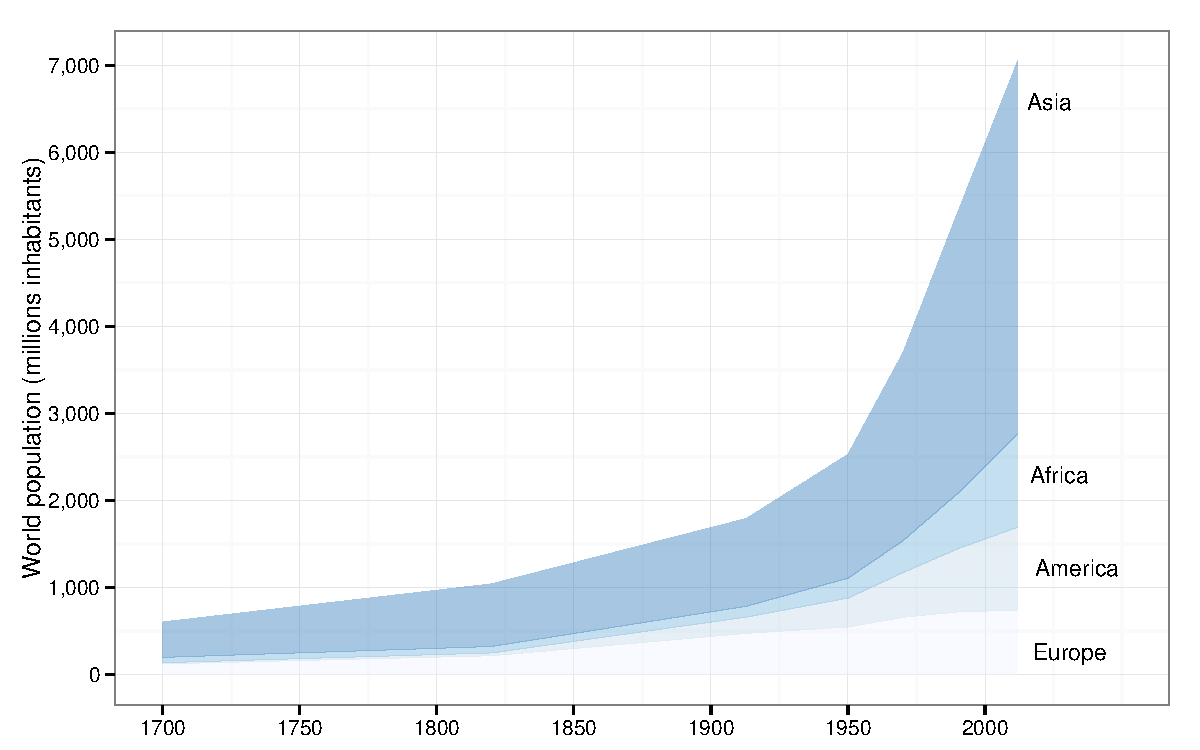
\includegraphics[width=1\linewidth]{figures/color/Figure_2_1} 

}



\end{knitrout}
\caption{World population rose from 600 million inhabitants in 1700 to 7 billion in 2012.}
\end{minipage}
\end{figure}
\end{frame}
%%%%%%%%%%%%%%%%%%%% Frame Here %%%%%%%%%%%%%%%%%%%%%%%%%%%%%%%%%%%%%%%%%%%%%%%%


%%%%%%%%%%%%%%%%%%%% Frame Here %%%%%%%%%%%%%%%%%%%%%%%%%%%%%%%%%%%%%%%%%%%%%%%%
\begin{frame}[label=Figure_2_1_b]
\frametitle{Figure 2.1: The growth of world population, 1700--2012}
\begin{figure}[t]
\begin{minipage}[b]{\textwidth}
\centering
\begin{knitrout}\footnotesize
\definecolor{shadecolor}{rgb}{0.969, 0.969, 0.969}\color{fgcolor}

{\centering 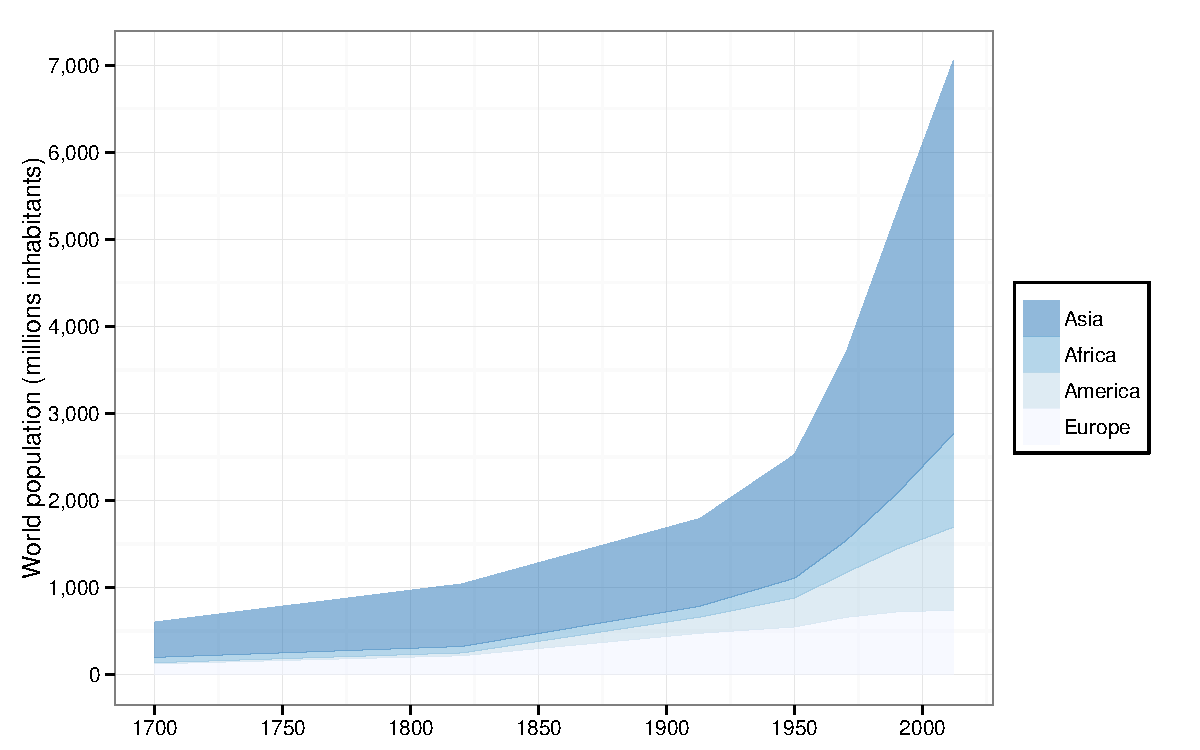
\includegraphics[width=1\linewidth]{figures/color/Figure_2_1_b} 

}



\end{knitrout}
\caption{World population rose from 600 million inhabitants in 1700 to 7 billion in 2012.}
\end{minipage}
\end{figure}
\end{frame}
%%%%%%%%%%%%%%%%%%%% Frame Here %%%%%%%%%%%%%%%%%%%%%%%%%%%%%%%%%%%%%%%%%%%%%%%%


%%%%%%%%%%%%%%%%%%%% Frame Here %%%%%%%%%%%%%%%%%%%%%%%%%%%%%%%%%%%%%%%%%%%%%%%%
\begin{frame}[label=Figure_2_2a]
\frametitle{Figure 2.2a: The growth rate of population from Antiquity to 2100}
\begin{figure}[t]
\begin{minipage}[b]{\textwidth}
\centering
\begin{knitrout}\footnotesize
\definecolor{shadecolor}{rgb}{0.969, 0.969, 0.969}\color{fgcolor}

{\centering 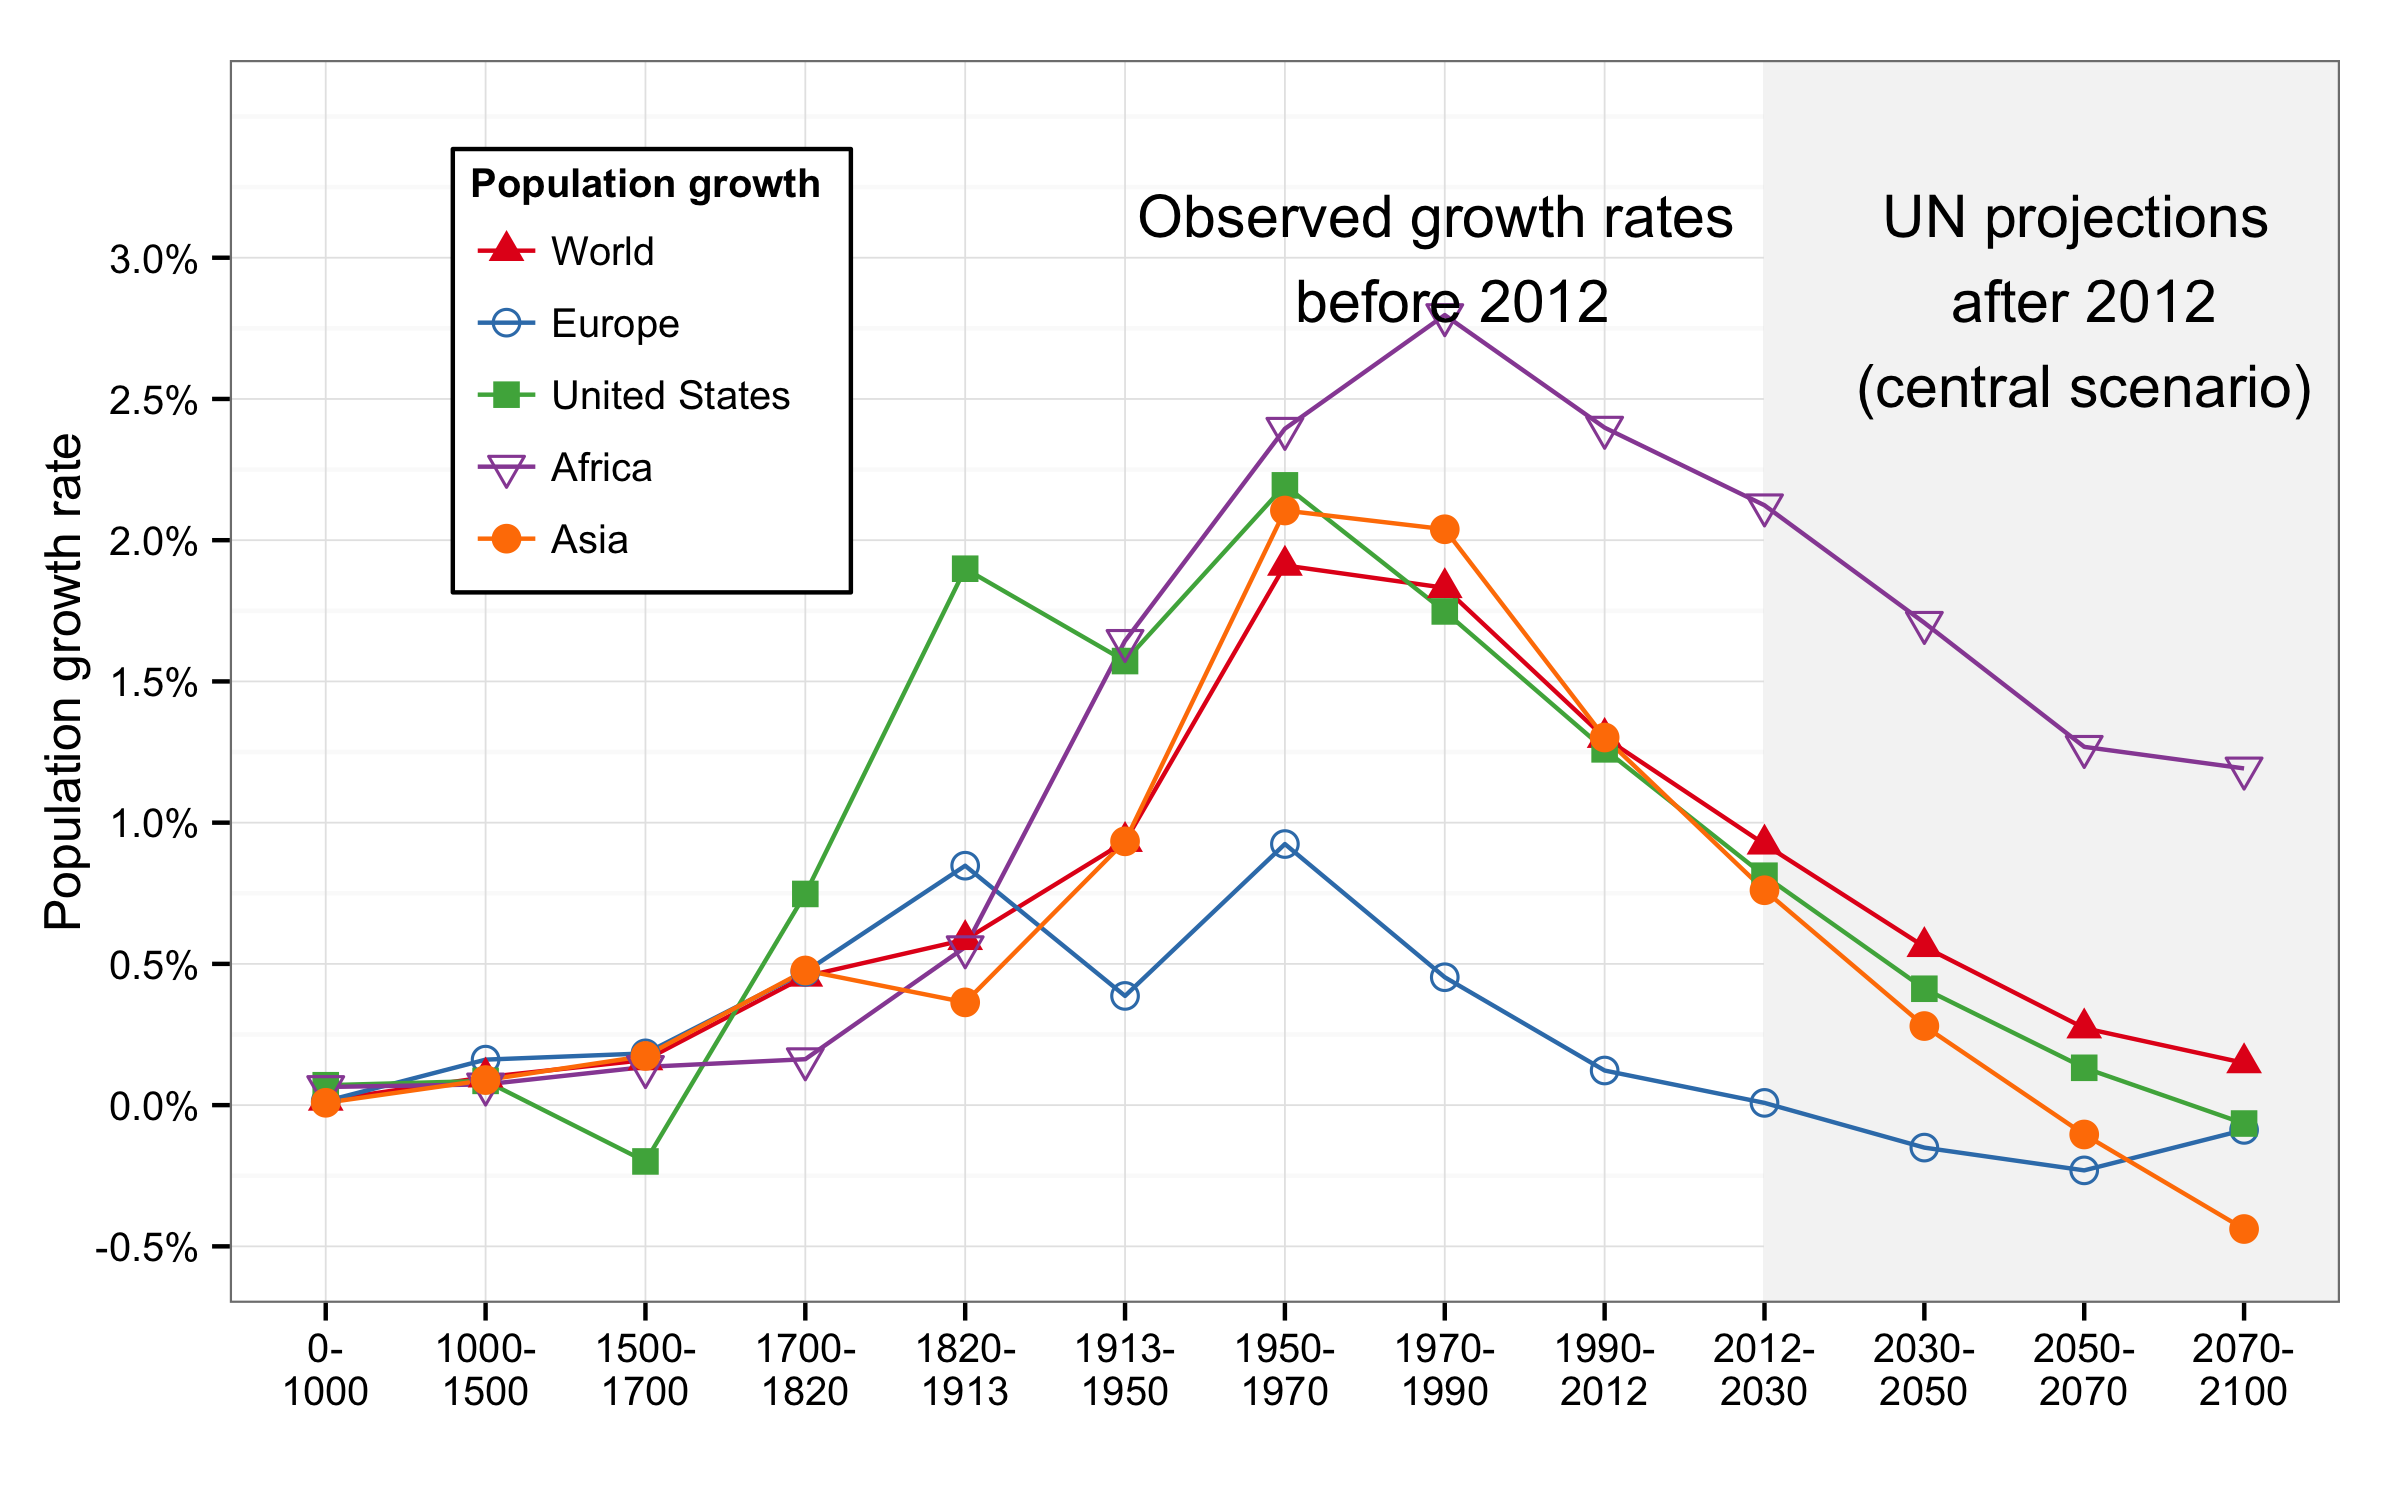
\includegraphics[width=1\linewidth]{figures/color/Figure_2_2a} 

}



\end{knitrout}
%\caption{}
\end{minipage}
\end{figure}
\end{frame}
%%%%%%%%%%%%%%%%%%%% Frame Here %%%%%%%%%%%%%%%%%%%%%%%%%%%%%%%%%%%%%%%%%%%%%%%%


%%%%%%%%%%%%%%%%%%%% Frame Here %%%%%%%%%%%%%%%%%%%%%%%%%%%%%%%%%%%%%%%%%%%%%%%%
\begin{frame}[label=Figure_2_2]
\frametitle{Figure 2.2: The growth rate of world population from Antiquity to 2100}
\begin{figure}[t]
\begin{minipage}[b]{\textwidth}
\centering
\begin{knitrout}\footnotesize
\definecolor{shadecolor}{rgb}{0.969, 0.969, 0.969}\color{fgcolor}

{\centering 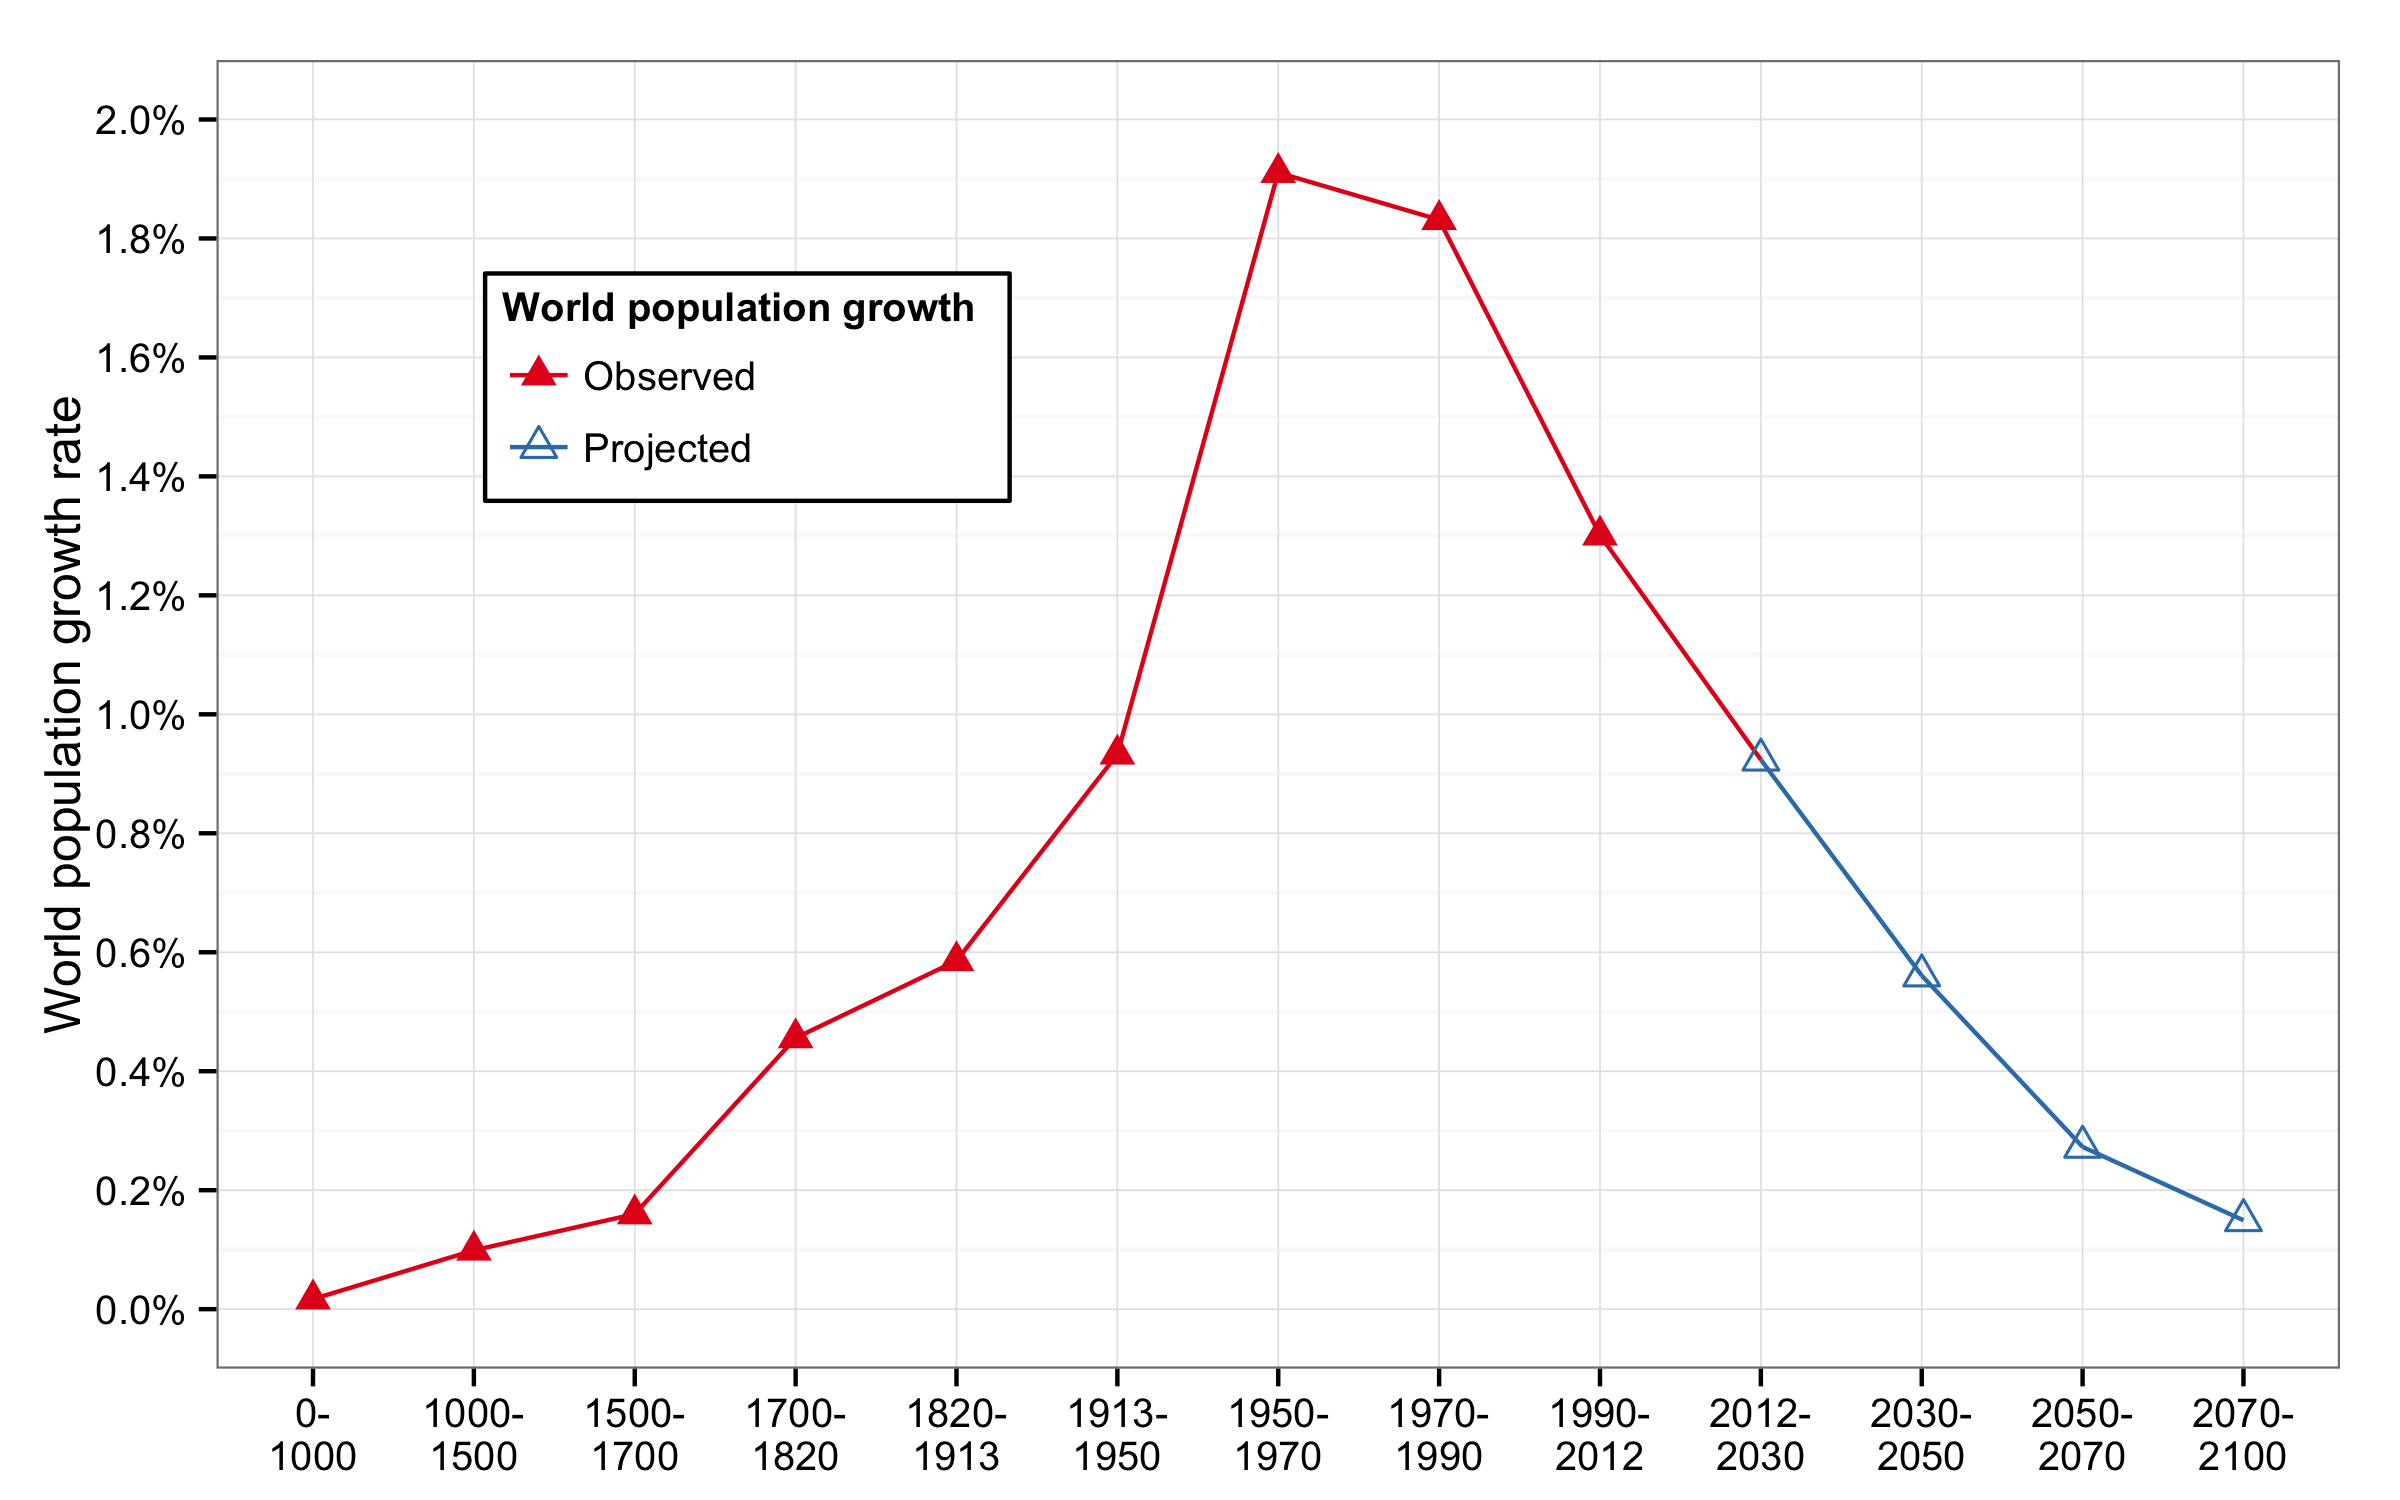
\includegraphics[width=1\linewidth]{figures/color/Figure_2_2} 

}



\end{knitrout}
\caption{The growth rate of world population was above 1 percent per year from 1950 to 2012 and should return toward 0 percent by the end of the twenty-first century.}
\end{minipage}
\end{figure}
\end{frame}
%%%%%%%%%%%%%%%%%%%% Frame Here %%%%%%%%%%%%%%%%%%%%%%%%%%%%%%%%%%%%%%%%%%%%%%%%


%%%%%%%%%%%%%%%%%%%% Frame Here %%%%%%%%%%%%%%%%%%%%%%%%%%%%%%%%%%%%%%%%%%%%%%%%
\begin{frame}[label=Figure_2_3]
\frametitle{Figure 2.3: The growth rate of per capita output since the Industrial Revolution}
\begin{figure}[t]
\begin{minipage}[b]{\textwidth}
\centering
\begin{knitrout}\footnotesize
\definecolor{shadecolor}{rgb}{0.969, 0.969, 0.969}\color{fgcolor}

{\centering 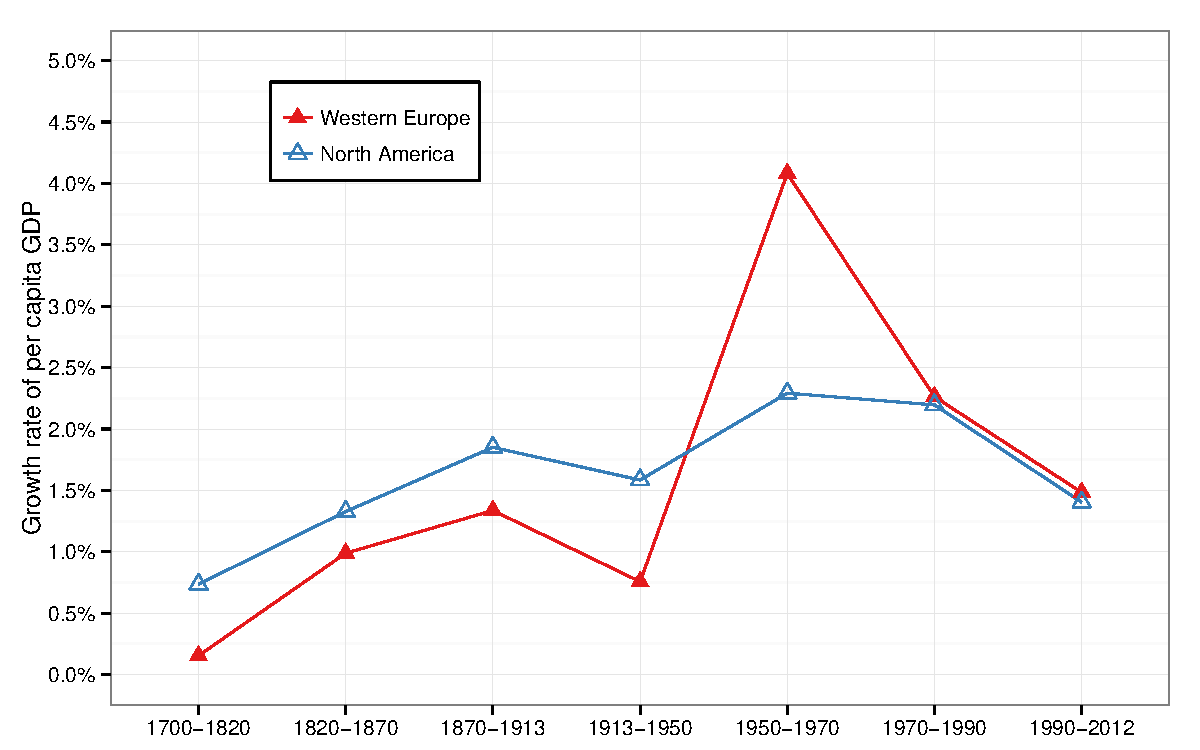
\includegraphics[width=1\linewidth]{figures/color/Figure_2_3} 

}



\end{knitrout}
\caption{The growth rate of per capita output surpassed 4 percent per year in Europe between 1950 and 1970, before returning to American levels.}
\end{minipage}
\end{figure}
\end{frame}
%%%%%%%%%%%%%%%%%%%% Frame Here %%%%%%%%%%%%%%%%%%%%%%%%%%%%%%%%%%%%%%%%%%%%%%%%


%%%%%%%%%%%%%%%%%%%% Frame Here %%%%%%%%%%%%%%%%%%%%%%%%%%%%%%%%%%%%%%%%%%%%%%%%
\begin{frame}[label=Figure_2_4]
\frametitle{Figure 2.4: The growth rate of world per capita output from Antiquity to 2100}
\begin{figure}[t]
\begin{minipage}[b]{\textwidth}
\centering
\begin{knitrout}\footnotesize
\definecolor{shadecolor}{rgb}{0.969, 0.969, 0.969}\color{fgcolor}

{\centering 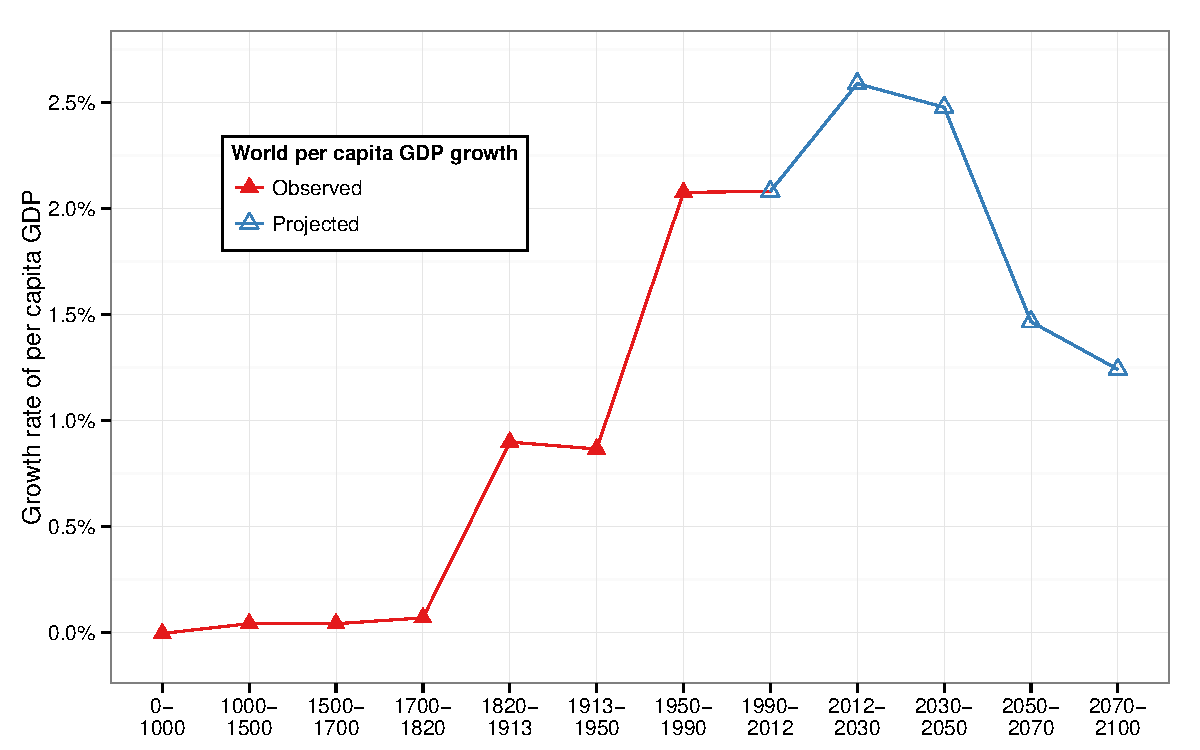
\includegraphics[width=1\linewidth]{figures/color/Figure_2_4} 

}



\end{knitrout}
\caption{The growth rate of per capita output surpassed 2 percent from 1950 to 2012. If the convergence process goes on, it will surpass 2.5 percent from 2012 to 2050, and then will drop below 1.5 percent.}
\end{minipage}
\end{figure}
\end{frame}
%%%%%%%%%%%%%%%%%%%% Frame Here %%%%%%%%%%%%%%%%%%%%%%%%%%%%%%%%%%%%%%%%%%%%%%%%


%%%%%%%%%%%%%%%%%%%% Frame Here %%%%%%%%%%%%%%%%%%%%%%%%%%%%%%%%%%%%%%%%%%%%%%%%
\begin{frame}[label=Figure_2_5]
\frametitle{Figure 2.5: The growth rate of world output from Antiquity to 2100}
\begin{figure}[t]
\begin{minipage}[b]{\textwidth}
\centering
\begin{knitrout}\footnotesize
\definecolor{shadecolor}{rgb}{0.969, 0.969, 0.969}\color{fgcolor}

{\centering 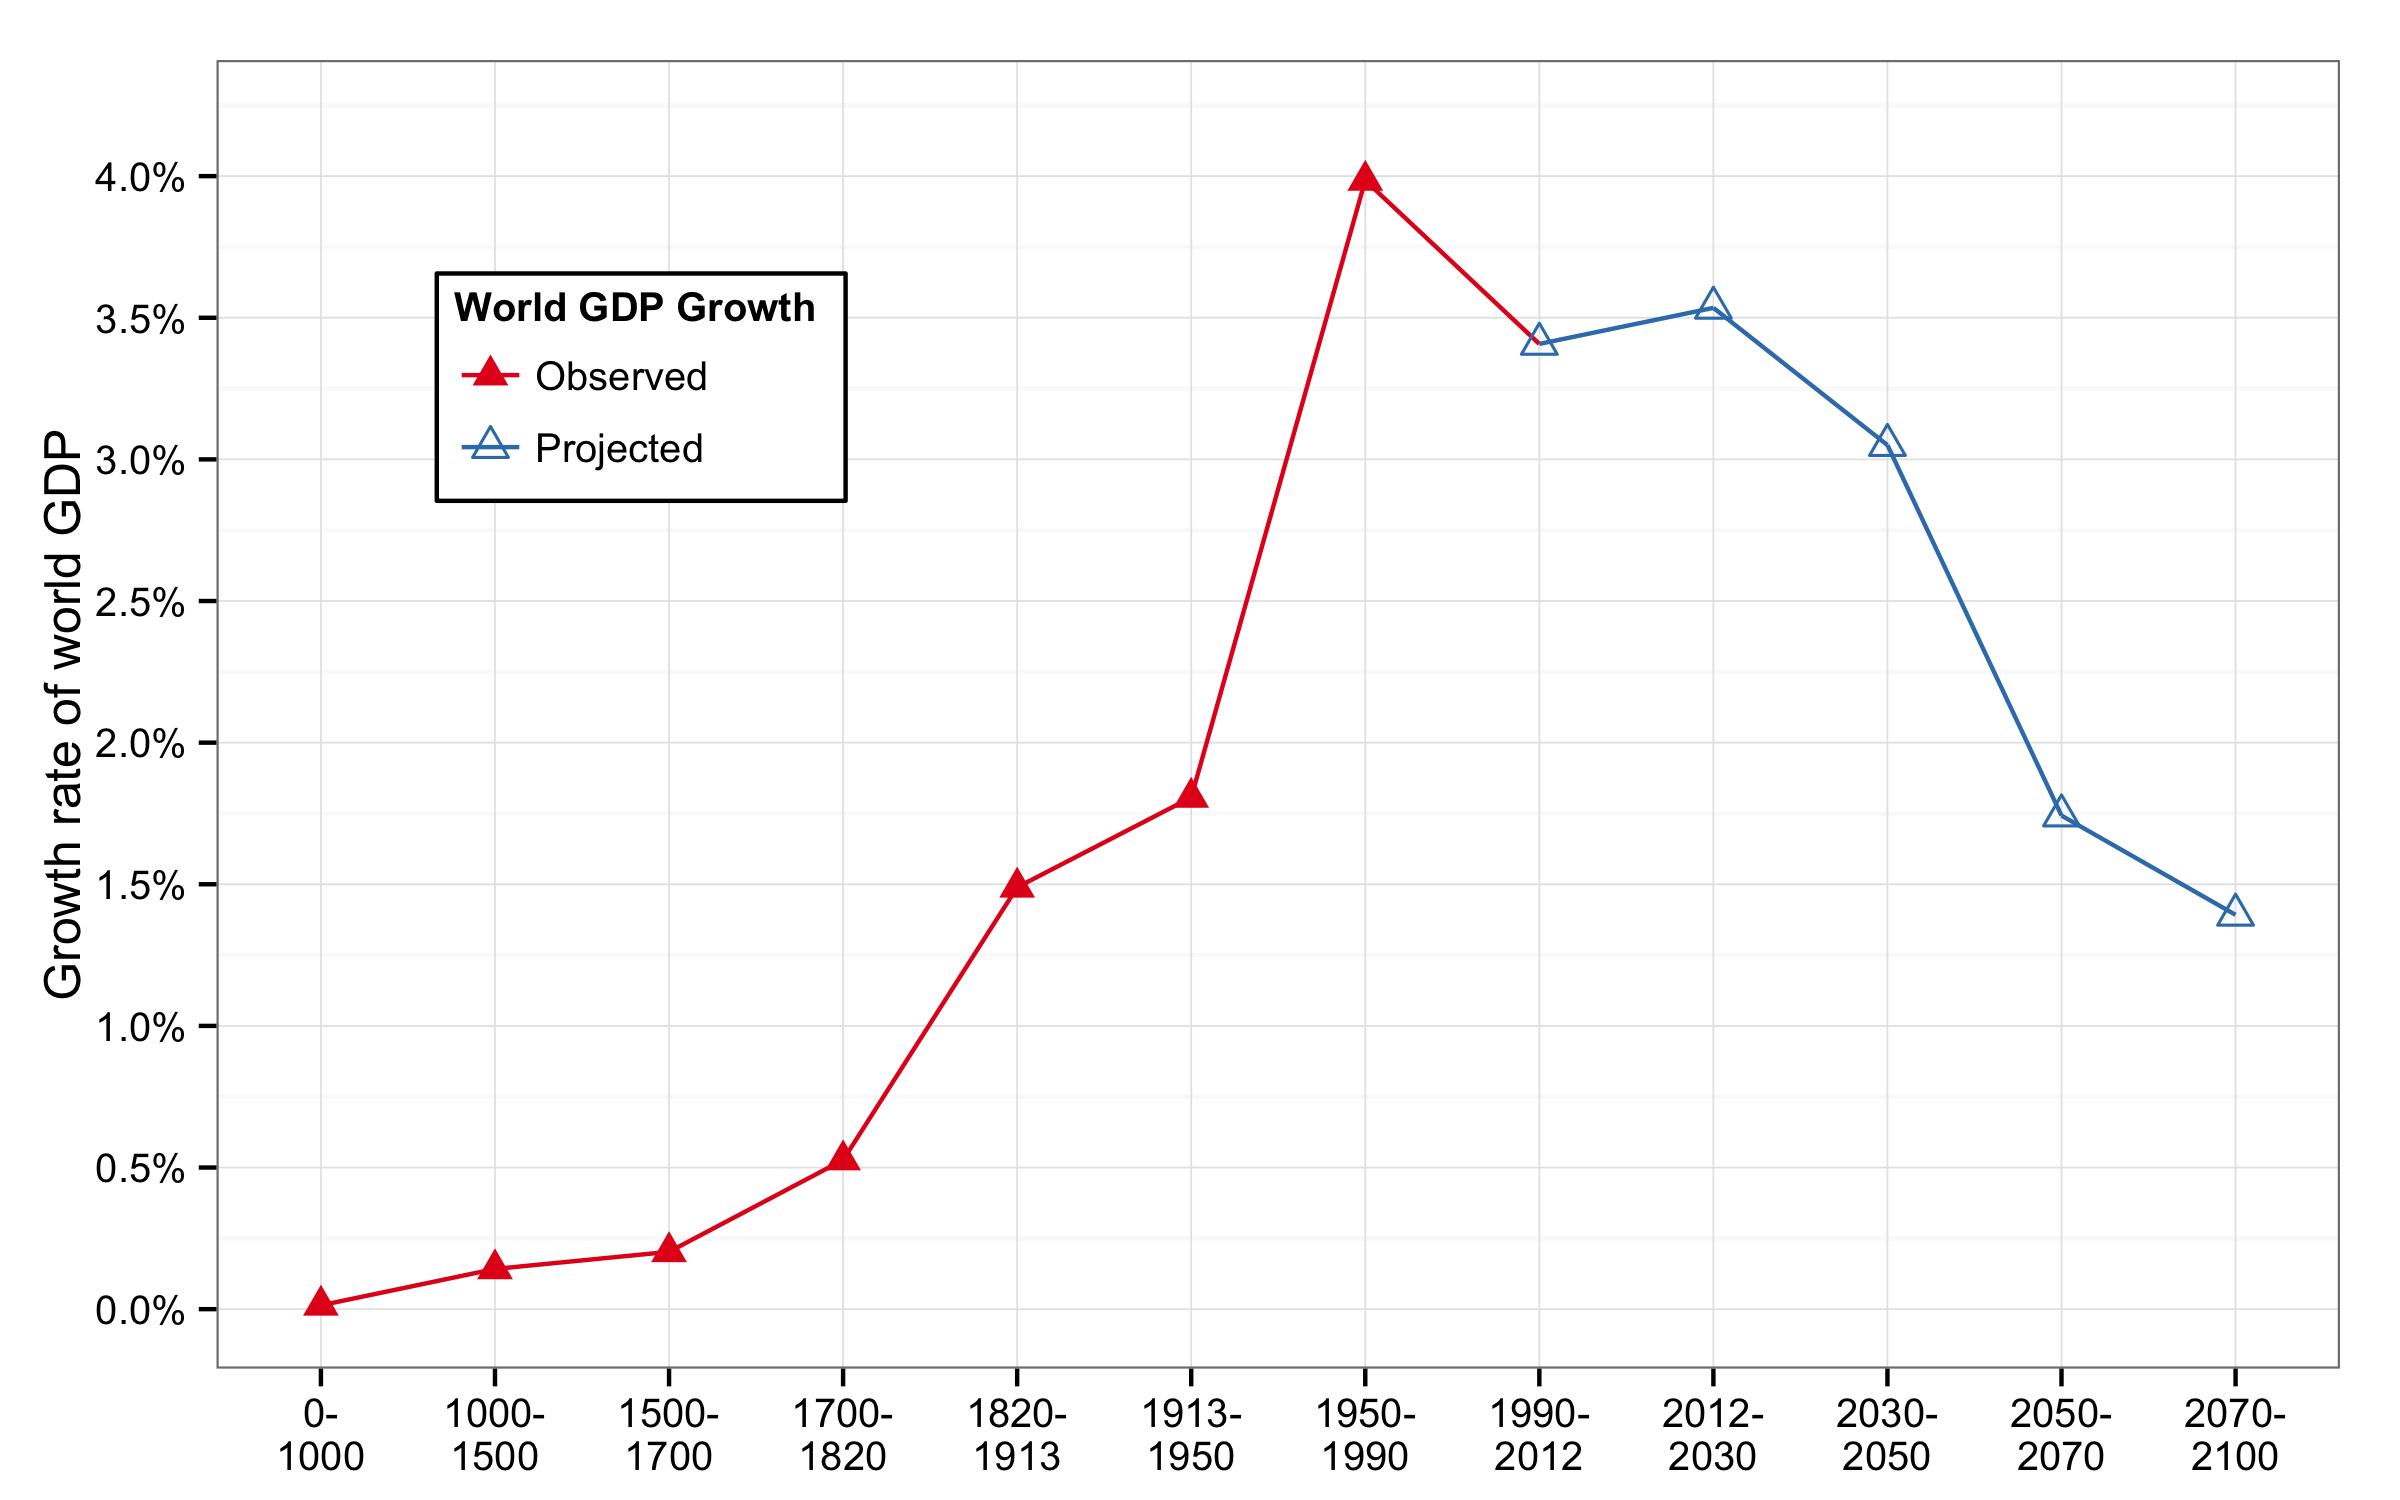
\includegraphics[width=1\linewidth]{figures/color/Figure_2_5} 

}



\end{knitrout}
\caption{The growth rate of world output surpassed 4 percent from 1950 to 1990. If the convergence process goes on, it will drop below 2 percent by 2050.}
\end{minipage}
\end{figure}
\end{frame}
%%%%%%%%%%%%%%%%%%%% Frame Here %%%%%%%%%%%%%%%%%%%%%%%%%%%%%%%%%%%%%%%%%%%%%%%%


%%%%%%%%%%%%%%%%%%%% Frame Here %%%%%%%%%%%%%%%%%%%%%%%%%%%%%%%%%%%%%%%%%%%%%%%%
\begin{frame}[label=Figure_2_6,fragile]
\frametitle{Figure 2.6. Inflation since the Industrial Revolution}
\begin{figure}[t]
\begin{minipage}[b]{\textwidth}
\centering
\begin{knitrout}\footnotesize
\definecolor{shadecolor}{rgb}{0.969, 0.969, 0.969}\color{fgcolor}

{\centering 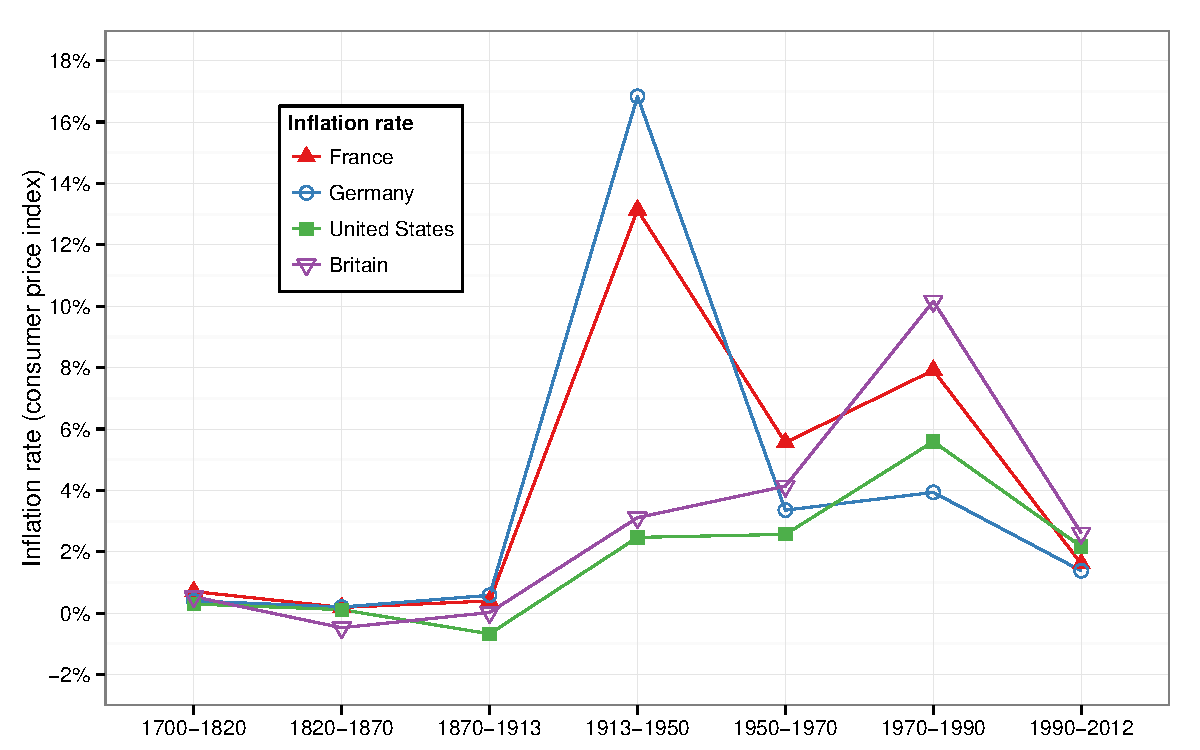
\includegraphics[width=1\linewidth]{figures/color/Figure_2_6} 

}



\end{knitrout}
\caption{Inflation in the rich countries was zero in the eighteenth and nineteenth centuries, high in the twentieth century, and roughly 2 percent a year since 1990.}
\end{minipage}
\end{figure}
\end{frame}
%%%%%%%%%%%%%%%%%%%% Frame Here %%%%%%%%%%%%%%%%%%%%%%%%%%%%%%%%%%%%%%%%%%%%%%%%


%%%%%%%%%%%%%%%%%%%% Frame Here %%%%%%%%%%%%%%%%%%%%%%%%%%%%%%%%%%%%%%%%%%%%%%%%
\begin{frame}[label=Figure_12_1]
\frametitle{Figure 12.1: }
\begin{figure}[t]
\begin{minipage}[b]{\textwidth}
\centering

\caption{.}
\end{minipage}
\end{figure}
\end{frame}
%%%%%%%%%%%%%%%%%%%% Frame Here %%%%%%%%%%%%%%%%%%%%%%%%%%%%%%%%%%%%%%%%%%%%%%%%


%%%%%%%%%%%%%%%%%%%% Frame Here %%%%%%%%%%%%%%%%%%%%%%%%%%%%%%%%%%%%%%%%%%%%%%%%
\begin{frame}[label=Figure_12_2]
\frametitle{Figure 12.2: }
\begin{figure}[t]
\begin{minipage}[b]{\textwidth}
\centering

\caption{.}
\end{minipage}
\end{figure}
\end{frame}
%%%%%%%%%%%%%%%%%%%% Frame Here %%%%%%%%%%%%%%%%%%%%%%%%%%%%%%%%%%%%%%%%%%%%%%%%


%%%%%%%%%%%%%%%%%%%% Frame Here %%%%%%%%%%%%%%%%%%%%%%%%%%%%%%%%%%%%%%%%%%%%%%%%
\begin{frame}[label=Figure_12_3]
\frametitle{Figure 12.3: }
\begin{figure}[t]
\begin{minipage}[b]{\textwidth}
\centering

\caption{.}
\end{minipage}
\end{figure}
\end{frame}
%%%%%%%%%%%%%%%%%%%% Frame Here %%%%%%%%%%%%%%%%%%%%%%%%%%%%%%%%%%%%%%%%%%%%%%%%


\againframe{Table_12_1}


\againframe{Table_12_2}


%%%%%%%%%%%%%%%%%%%% Frame Here %%%%%%%%%%%%%%%%%%%%%%%%%%%%%%%%%%%%%%%%%%%%%%%%
\begin{frame}[label=InequalityUSA]
\frametitle{3. Inequality in America}
\framesubtitle{``meritocratic extremism''}
\begin{itemize}
\item
Inequality in America = a different structure as in Europe: 
\textbf{more egalitarian in some ways, more inegalitarian in some other dimensions}.
\item
The New World in the 19th century: the land of opportunity (capital accumulated in the past mattered much less than in Europe; perpetual demographic growth as a way to reduce the level of inherited wealth and wealth concentration)... and also the land of slavery.
\item 
Northern US were in many ways more egalitarian than Old Europe; but Southern US were more inegalitarian.
\item 
We still have the same ambiguous relationship of America with inequality today: in some ways more merit-based; in other ways more violent (prisons).
\end{itemize}
\end{frame}
%%%%%%%%%%%%%%%%%%%% Frame Here %%%%%%%%%%%%%%%%%%%%%%%%%%%%%%%%%%%%%%%%%%%%%%%%


%\againframe{Figure_3_2}


%%%%%%%%%%%%%%%%%%%% Frame Here %%%%%%%%%%%%%%%%%%%%%%%%%%%%%%%%%%%%%%%%%%%%%%%%
\begin{frame}[label=Figure_4_6]
\frametitle{Figure 4.6: }
\begin{figure}[t]
\begin{minipage}[b]{\textwidth}
\centering

\caption{.}
\end{minipage}
\end{figure}
\end{frame}
%%%%%%%%%%%%%%%%%%%% Frame Here %%%%%%%%%%%%%%%%%%%%%%%%%%%%%%%%%%%%%%%%%%%%%%%%


\againframe{Figure_5_2}


%%%%%%%%%%%%%%%%%%%% Frame Here %%%%%%%%%%%%%%%%%%%%%%%%%%%%%%%%%%%%%%%%%%%%%%%%
\begin{frame}[label=Figure_4_10]
\frametitle{Figure 4.10: }
\begin{figure}[t]
\begin{minipage}[b]{\textwidth}
\centering

\caption{.}
\end{minipage}
\end{figure}
\end{frame}
%%%%%%%%%%%%%%%%%%%% Frame Here %%%%%%%%%%%%%%%%%%%%%%%%%%%%%%%%%%%%%%%%%%%%%%%%


%%%%%%%%%%%%%%%%%%%% Frame Here %%%%%%%%%%%%%%%%%%%%%%%%%%%%%%%%%%%%%%%%%%%%%%%%
\begin{frame}[label=Figure_4_11]
\frametitle{Figure 4.11: }
\begin{figure}[t]
\begin{minipage}[b]{\textwidth}
\centering

\caption{.}
\end{minipage}
\end{figure}
\end{frame}
%%%%%%%%%%%%%%%%%%%% Frame Here %%%%%%%%%%%%%%%%%%%%%%%%%%%%%%%%%%%%%%%%%%%%%%%%


%%%%%%%%%%%%%%%%%%%% Frame Here %%%%%%%%%%%%%%%%%%%%%%%%%%%%%%%%%%%%%%%%%%%%%%%%
\begin{frame}[label=USAvEU]
\frametitle{America Versus Europe}
\begin{itemize}
\item
The US distribution of income has become more unequal than in Europe over the course of the 20th century; it is now as unequal as pre--WW1 Europe.
\item 
But the structure of inequality is different: US 2013 has less wealth inequality than Europe 1913, but higher inequality of labor income.
\end{itemize}
\end{frame}
%%%%%%%%%%%%%%%%%%%% Frame Here %%%%%%%%%%%%%%%%%%%%%%%%%%%%%%%%%%%%%%%%%%%%%%%%


%%%%%%%%%%%%%%%%%%%% Frame Here %%%%%%%%%%%%%%%%%%%%%%%%%%%%%%%%%%%%%%%%%%%%%%%%
\begin{frame}[label=Figure_10_6]
\frametitle{Figure 10.6: }
\begin{figure}[t]
\begin{minipage}[b]{\textwidth}
\centering

\caption{.}
\end{minipage}
\end{figure}
\end{frame}
%%%%%%%%%%%%%%%%%%%% Frame Here %%%%%%%%%%%%%%%%%%%%%%%%%%%%%%%%%%%%%%%%%%%%%%%%


\againframe{Figure_8_5}


\againframe{Figure_9_8}


%%%%%%%%%%%%%%%%%%%% Frame Here %%%%%%%%%%%%%%%%%%%%%%%%%%%%%%%%%%%%%%%%%%%%%%%%
\begin{frame}[label=MeritVNorms]
\frametitle{Merit or Social Norms?}
\begin{itemize}
\item
Higher inequality of labor income in the US could reflect higher inequality in education investment; but it also reflects a huge rise of top executive compensation that it very hard to explain with education and productivity reasoning alone.
\item 
In the US, this is sometime described as more merit--based: the rise of top labor incomes makes it possible to become rich with no inheritance ($\simeq$~Napoleonic «préfets»)
\item 
\textbf{Problem: this can be the worst of all worlds for those who are neither top income earners nor top successors}: they are poor, and they are depicted as dump \& undeserving (by contrast, nobody was trying to depict Ancien Regime inequality as fair!).
\item 
It is unclear whether rise of top incomes has a lot to do with merit or productivity: sharp decline in top tax rates \& rise of CEO bargaining power are more convincing explanations; chaotic US history of social norms regarding inequality.
\end{itemize}
\end{frame}
%%%%%%%%%%%%%%%%%%%% Frame Here %%%%%%%%%%%%%%%%%%%%%%%%%%%%%%%%%%%%%%%%%%%%%%%%


\againframe{Figure_14_1}


\againframe{Figure_14_2}


\againframe[shrink=7]{Conclusions_1}



\end{document}

